% ################################################################
% # Recife, 18 February 2011                                     #
% # Polytechnic School of Pernambuco - University of Pernambuco  #
% # Course: Computer Engineer                                    #
% # Author: Marcos Alvares Barbosa Junior                        #
% #                                                              #
% # UPE-POLI MSc Thesis Template    V0.1                         #
% ################################################################
%   TODO:
%     #1:  Move the Default Configuration section to a separeted file
%     #2:  Create a LaTeX Class
%     #3:  Create examples of Symbols, Equations, Tables, Figures, sections and sub-sections ...
%     #4:  Discat all specific contents (: replace the thesis title with an generic value like: "Here You Put Your Thesis Title")
%     #5:  Verify ununsed packages
%
\documentclass[a4paper,12pt]{upethesis}
%
%\fancyhead[L]{
%    \parbox{2cm}{
\includegraphics[scale=0.4]{image/poli_logo_white.jpg}}
%}
%
%\fancyhead[R]{
%    \parbox{1cm}{
\includegraphics[scale=0.4]{image/upe_logo_white.jpg}}
%}

\fancyfoot[R]{
    \footnotesize {\color{gray}{\thepage}}
}


\begin{document}
  % Thesis Pre-textual elements [START]
\begin{titlepage}

  \begin{center}
  
\includegraphics[scale=0.17]{image/UPE_brasao}\\
	\textbf{Universidade de Pernambuco}\\
	\textbf{Escola Politécnica de Pernambuco}\\
    \textbf{Programa de Pós-Graduação em Engenharia da Computação}\\[3cm]

    Carlos Henrique Maciel Sobral Timóteo\\[2cm]


    {\large \textbf{Metodologia para a Análise Quantitativa de Riscos no Gerenciamento de Projetos de Software}}\\[3cm]

    Dissertação de Mestrado\\[2cm]
  \end{center}


\begin{center}
  {\color{white} xx}\vfill
  Recife, Julho de 2014
\end{center}

\end{titlepage}

\begin{titlepage}
%    \begin{figure}[ht]
%    \mbox{
\includegraphics[scale=0.4]{image/poli_logo.jpg}}\hfill
%    \mbox{
\includegraphics[scale=0.4]{image/upe_logo.jpg}}
%  \end{figure}
  \begin{center}
	
\includegraphics[scale=0.17]{image/UPE_brasao}\\
	\textbf{Universidade de Pernambuco}\\
	\textbf{Escola Politécnica de Pernambuco}\\
    \textbf{Programa de Pós-Graduação em Engenharia da Computação}\\[3cm]

    Carlos Henrique Maciel Sobral Timóteo\\[2cm]
{
\Large
    \textbf{A Methodology for Quantitative Risk Analysis in Project Management Software}\\[2cm]
}
  \end{center}

\noindent\adjustbox{varwidth=10cm,right,margin=0pt \bigskipamount}{% (`margin` adds a vertical skip above and belo)
        Dissertação de Mestrado apresentada ao
            Programa de Pós-Graduação em Engenharia
            da Computação da Universidade de
            Pernambuco como requisito parcial para
            obtenção do título de Mestre em Engenharia
            da Computação.
}

  \begin{flushright}
    Prof. Dr. Sérgio Murilo Maciel Fernandes\\
    Orientador\\
    \qquad\\
    Prof. Dr. Mêuser Jorge Valença\\
    Coorientador\\
  \end{flushright}

\begin{center}
  {\color{white} xx}\vfill
  Recife, June de 2014
\end{center}

\end{titlepage}


%\begin{center}
  {\color{white} xx}\vfill
  REVIEWER NOTES.\\
  Recife, Mar 2014
\end{center}
\newpage 
\pagenumbering{gobble}
\begin{flushbottom}
\textbf{DEDICATION}
\\
\\
Firstly, I want to thank God for giving me health and peace, and to make everything possible. I have to thank a lot to my father for his understanding and to my mother for her unconditional support. A special thanks to my brother by his cheer, support and for motivating me during this journey.

I am very grateful to my supervisor, Professor Carmelo, for all learning and guidance. When working by his side, I found my vocation as a professor. He is my example of professor, researcher and advisor. What he taught me is not found in books. He taught me to believe in the potential of students, motivate them, let them excited during classes and respect people. Thus, he won the admiration of all the people. I thank all the professors of the Postgraduate Program in Computing Engineering for their contribution to my development. I also thank the undergraduate student Sergio Ribeiro due to our successful partnership.

I want to thank my friends of now and forever, Cesar, Caio, Thiago, George, Victor and Silvia for all the support. Despite the distance, they always were with me. It is always good to make new friends. Finally, I want to thank all the new friends and colleagues that I did during these two years, Paulo Roger, Debora, Marcelo, Renatha, Rodrigo (teoria) because my master's degree would not be the same without their support.

A special thank to the secretaries Ana Georgina and Julia by their conversations and help. They welcomed me with a smile when I arrived and said "Hi" always.

I know that I may lose contact with most of these people due the circumstances, but I want to state my thanks for they having entered into my life.
\end{flushbottom}
\newpage

\begin{flushbottom}
\textbf{EPIGRAPH}
\\
\\
\\
\textit{``Everyone here has the sense that right now is one of those moments when we are influencing the future.''} Steve Jobs
\\
\\
\\
\\
\\
\\
\\
\\
\\
\\Recife, July 2012
\end{flushbottom}
\newpage

\pagenumbering{roman}
\setcounter{page}{4}
%DESCOMENTAR...
% % % % % % % % %
\begin{flushbottom}
\begin{flushleft}
{\huge \textbf{Resumo}}
\linebreak
\end{flushleft}
Muitos projetos de desenvolvimento de software/ti finalizam sem alcançar todos os seus objetivos. Segundo estudos já realizados, somente um quarto dos projetos de software têm sucesso imediato, e bilhões de dólares são perdidos anualmente por meio de falhas ou projetos que não cumprem a entrega dos benefícios prometidos. Além disso, ainda há algumas dificuldades na interpretação do conceito de risco e na aplicação de métodos para a análise de risco de forma eficiente e precisa, conforme descrito nesta dissertação. Isso ocorre devido a vários fatores: falta de habilidade para manusear as ferramentas existentes; falta de conhecimento dos benefícios obtidos pela gestão de risco, bem como as limitações encontradas nas ferramentas sugeridas como boas práticas; a ausência de estudos na indústria que comprovem o valor de cada técnica e a dificuldade na obtenção de uma base de dados de riscos adequada.

Dentre as técnicas convencionais na literatura, há a Simulação de Monte Carlo (SMC) e Análise PERT. Na SMC, as simulações podem levar a resultados enganosos se entradas inapropriadas, através da inserção de parâmetros manualmente, forem inseridas no modelo. Além disso, como ela não pode modelar correlações entre riscos, então os números que surgem em cada sorteio são aleatórios. Na Análise PERT, por sua vez, como há necessidade da opinião de um especialista, basta inserir valores de entrada errôneos para gerar resultados incoerentes.

Nesse trabalho, uma base de dados especial, chamada PERIL, é utilizada e é proposta uma metodologia para a análise de risco cujo diferencial é encontrar uma Rede Neural Artificial que seja mais eficiente e precisa que as técnicas convencionais até então utilizadas (SMC e Análise PERT), independentemente da base de dados a ser empregada. Perceptron de Múltiplas Camadas (MLP), Máquina de Vetor de Suporte, Redes com Função de Base Radial, um Sistema Adaptativo \textit{Neuro-Fuzzy}, Modelos de Regressão Linear, Simulação de Monte Carlo e Análise PERT foram as técnicas avaliadas. Em seguida, são conduzidos experimentos para determinar qual o método mais eficiente e preciso para a estimativa do impacto de risco relativo ao número de dias atrasados para a finalização de uma atividade, baseada em informações da PERIL. Por fim, um intervalo de confiança pôde ser obtido para uma determinada previsão.

Os resultados mostram que uma das variações da MLP (MLPRegressor) obteve melhores resultados que qualquer outra técnica. Além disso, comprova-se que a Simulação de Monte Carlo apresenta os piores resultados ainda que se compare com modelos de regressão linear simples. Por fim, a análise PERT mostra ser bastante eficiente quando se utiliza a opinião especializada e uma base de dados de riscos como a PERIL.
\\
\\
\textbf{Palavras-chave:} \\ Gerenciamento de Projetos, Análise de Riscos, PERIL, Redes Neurais Artificiais, Simulação de Monte Carlo, Análise PERT.\end{flushbottom}
\newpage

\begin{flushbottom}
\begin{flushleft}
{\huge \textbf{Abstract}}
\linebreak
\end{flushleft}
Many software/it projects end in failure, without reaching their objectives. According to previous studies, only a quarter of software/it projects have immediate success, and billions of dollars are lost annually through failures or projects that do not meet the delivery of promised benefits. Moreover, there are still some difficulties in the interpretation of the concept of risk and application of methods for risk analysis efficiently and accurately. This is due to several factors: lack of ability to handle existing tools; lack of knowledge of the benefits from risk management as well as limitations found in the tools suggested as good practice; the lack of studies in the industry proving the value of each technique and the difficulty in obtaining a database of proper risk. 

Among traditional techniques in literature, there are Monte Carlo Simulation (MCS) and PERT Analysis. In MCS, simulations can return misleading results if inappropriate inputs, through manual insertion of parameters, are incorporated into the model. Besides, as it can not model correlations between risks, then the numbers appearing in each drawing are random. In PERT analysis, in turn, as there is a need for specialized opinion, just enter erroneous input values to generate inconsistent results.

In this work, a special database, called PERIL, is used and is proposed a methodology for risk analysis whose diferential is to find an Artificial Neural Network which is more efficient and accurate than standard techniques previously used such as MCS and PERT, regardless of the database employed. Multilayer Perceptron, Support Vector Machine, Radial Basis Function Networks, an Adaptive Neuro-Fuzzy System, Linear Regression Models, Monte Carlo Simulation and PERT Analysis techniques were evaluated. Then, experiments are conducted to determine which is a more efficient and accurate method for risk impact estimation related to the number of delayed days to finish an activity based on PERIL. Finally, a confidence interval could be obtained for a given prediction. 

The results show that a MLP variation (MLPRegressor) has better results than any other technique. Furthermore, it was proven that Monte Carlo Simulation shows the worst results still compared with Linear Regression Models. Finally, PERT analysis shows to be quite efficient when using expert judgment and a risk database as PERIL.
\\
\\
\textbf{Keywords:} \\ Project Management, Risk Analysis, PERIL, Artificial Neural Networks, Monte Carlo Simulation, PERT Analysis.\end{flushbottom}
\newpage

\tableofcontents                                                           % CONTENTS
\listoffigures\addcontentsline{toc}{chapter}{Lista de Figuras}              % LIST OF FIGURES
%\chapter*{Symbols List\hfill} \addcontentsline{toc}{chapter}{Symbols List}
%\newpage
\chapter*{Lista de Siglas\hfill} \addcontentsline{toc}{chapter}{Lista de Siglas}
\listofacronyms
\newpage
\chapter*{Lista de Símbolos\hfill} \addcontentsline{toc}{chapter}{Lista de Símbolos}
\listofsymbols
\newpage
 %\addcontentsline{toc}{chapter}{Figures List}
 %\listoffigures 
 %\newpage
\listofalgorithms\addcontentsline{toc}{chapter}{Lista de Algoritmos}
\newpage
\listoftables\addcontentsline{toc}{chapter}{Lista de Tabelas}
\newpage
% % % % % % % % % 
% % % % % % % %
%\newpage
%\addcontentsline{toc}{chapter}{Lista de Figuras}
%\listoffigures 
%\newpage
%\listoftables\addcontentsline{toc}{chapter}{Lista de Tabelas}                % LIST OF TABLES
%%\listofsymbols                                                             % LIST OF SYMBOLS
%\newpage
%\chapter*{Lista de Símbolos\hfill} \addcontentsline{toc}{chapter}{Lista de Símbolos}
%\listofsymbols
%\newpage
%\chapter*{Lista de Siglas\hfill} \addcontentsline{toc}{chapter}{Lista de Siglas}
%\listofacronyms
%\newpage
%%\addcontentsline{toc}{chapter}{Lista de Símbolos}
%%\newpage
%\listofalgorithms\addcontentsline{toc}{chapter}{Lista de Algoritmos}
%\newpage
% % % % % % % %
\setcounter{page}{1}
\pagenumbering{arabic}


% Thesis Chapters [START]
  \chapter{Introdução}\label{cap:introduction}

Quão arriscados são os projetos de \textit{software}? Diversos estudos sobre a efetividade de técnicas de previsão de custo, escopo, cronograma; \textit{surveys} com profissionais em \textit{software} na indústria; e análise de portfólio de projetos foi realizada para responder essa questão \cite{budzier2013double} \cite{flyvbjerg2013quality} \cite{jones1998estimating} \cite{CHAOS2009} \cite{jones2008applied} \cite{molokken2003review}. No entanto, não há um consenso.
%How risky are software projects? Several studies about effectiveness of software cost, scope, schedule estimation techniques; surveys from software professionals in industry; and analysis of projects portfolio have been done to answer this question \cite{budzier2013double}. However, there is not a consensus. 

Todos os projetos envolvem risco. Há sempre pelo menos algum nível de incerteza no resultado de um projeto, independentemente do que o gráfico de Gannt \cite{maylor2001beyond} pareça indicar. Projetos de alta tecnologia são particularmente arriscados, por uma série de motivos. Primeiro, há uma grande variedade de projetos técnicos. Esses projetos tem objetivos e aspectos únicos que os diferem significativamente dos trabalhos anteriores, além de apresentar um ambiente de projetos que evolue rapidamente. Além disso, projetos técnicos são frequentemente ``enxutos", ou seja, desafiados a trabalhar com financiamento, pessoal e equipamentos inadequados. Para piorar a situação, há uma expectativa generalizada que não corresponde à realidade de que por mais rápido que tenha sido o último projeto, o próximo deve ser ainda mais rápido \cite{kendrick2003identifying}.
%Every project involves risk. There is always at least some level of uncertainty in a project's outcome, regardless of what the Gantt chart on the wall seems to imply. High-tech projects are particularly risky, for a number of reasons. First, technical projects are high varied. These projects have unique aspects and objectives that significantly differ from previous work, and the environment for technical projects evolve quickly. In addition, technical projects are frequently "lean", challenged to work with inadequate funding, staff and equipment. To make matters worse, there is a pervasive expectation that however fast the last project may have been, the next one should be even quicker \cite{kendrick2003identifying}.

Projetos que tiveram sucesso geralmente conseguiram isso porque duas das ações tomadas pelos seus líderes foram determinantes. Primeiro, eles reconheceram que alguns dos trabalhos em qualquer projeto, mesmo projetos de alta tecnologia, não são novos. Nos trabalhos por eles desenvolvidos as notas, registros e lições aprendidas em projetos anteriores puderam ser utilizados como um roteiro para identificar, e em muitos casos evitar, muitos problemas potenciais. Segundo, eles planejaram com afinco o trabalho do projeto, especialmente as partes que exigiam inovação, para possibilitar a compreensão dos desafios futuros e antecipar muitos dos riscos \cite{kendrick2003identifying}.
%Projects that succeed generally do so because their leaders do two things well. First, they recognize that a few of the work on any project, even a high-tech project, is not new. For this work, the notes, records, and lessons learned on earlier projects can be a road map for identifying, and in many cases avoiding, many potential problems. Second, they plan project work thoroughly, especially the portions that require innovation, to understand the challenges ahead and to anticipate many of the risks \cite{kendrick2003identifying}.

Alguns benefícios da boa gestão de riscos de projetos de software são apresentados abaixo. Tais fatores podem determinar o sucesso dos projetos \cite{HIGUERAHAIMES1996} \cite{PMBOK2008}:
%Some benefits of good risk management of software projects are presented above. Such factors may determine the success of projects \cite{HIGUERAHAIMES1996} \cite{PMBOK2008}. 

\begin{itemize}
\item redução de custos incorridos com mudanças no software;
\item desenvolvimento de um plano de respostas a eventos inesperados, conhecido como plano de contingência de riscos;
\item previsão da probabilidade da ocorrência de eventos indesejados;
\item seguimento das linhas de base de custo, cronograma e qualidade.
\end{itemize}
%\begin{enumerate}
%\item reduction of costs associated with changes in software;
%\item development of a response plan to unexpected events, i.e., a contingency risk plan; 
%\item prediction of likelihood of undesired events;
%\item tracking the baselines of cost, schedule and quality.
%\end{enumerate}

\section{Motivação}

Em 2009, o CHAOS Report \cite{CHAOS2009} mostrou que 32\% dos projetos de software alcançaram sucesso, foram entregues no prazo, de acordo com o orçamento estabelecido e com os requisitos prometidos; 44\% dos projetos foram desafiados, em que o prazo ou o orçamento ou os requisitos não foram cumpridos; não menos importante, 24\% dos projetos falharam e foram cancelados no Mundo. Isso ocorre devido aos riscos envolvidos nas atividades do projeto e a um gerenciamento de riscos ausente ou deficiente \cite{ISLAM2009}. 
%In 2009, CHAOS Report \cite{CHAOS2009} showed that 32\% of projects achieved success - were delivered on time, on budget and with the promised requirements -; 44\% of the projects were challenged - or schedule or budget or requirements were not fulfilled; not least, 24\% of projects failed and were canceled. That is due to the risks involved in project activities and to a absent or defective software risk management \cite{ISLAM2009}.

Schmidt e outros autores \cite{schmidt2001identifying} notaram que muitos dos projetos de desenvolvimento de \textit{software} terminavam sem alcançar todos os objetivos. Eles mostraram que cerca de 25\% de todos os projetos de software são cancelados e cerca de 80\% de todos os projetos de software ultrapassaram seus orçamentos, excedendo-os em 50\% na média. Paul Bannerman \cite{bannerman2008risk} afirma que pesquisas na indústria sugerem que somente um quarto dos projetos de software tem sucesso imediato, e bilhões de dólares são perdidos anualmente por meio de falhas ou projetos que não cumprem a entrega dos benefícios prometidos. Além disso, o autor mostra evidências de que isso é um assunto global, impactando organizações do setor privado e público \cite{KPMG2005}.
%Schmidt et al. \cite{schmidt2001identifying} have noticed that many software development projects end in failure. They showed that around 25\% of all software projects are canceled outright and as many as 80\% of all software projects run over their budget, exceeding it by 50\% in average. Paul Bannerman \cite{bannerman2008risk} states that industry surveys suggest that only a quarter of software projects succeed outright, and billions of dollars are lost annually through project failures or projects that do not deliver promised benefits. Moreover, the author shows evidences that it's a global issue, impacting private and public sector organizations \cite{KPMG2005}.

A previsão de possíveis eventos a curto, médio e longo prazos muitas vezes é falha. Ao analisar os riscos e as incertezas, os gerentes de projeto comumente confiam na própria intuição, em vez de utilizarem a lógica e uma análise detalhada. No entanto, o pensamento intuitivo é frequentemente alvo de ilusões, que causam erros previsíveis e decisões eventualmente não embasadas. O método para conciliar o efeito dessas ilusões é uma avaliação sistemática dos riscos e esforços na mitigação dos mesmos através de métodos analíticos.
%Predict possible events in short, medium and long term is often failure. By analyzing risks and uncertainties, project managers commonly rely on intuition rather than logic and analysis. However, intuitive thinking is often subject to delusions, causing predictable mental errors and eventually poor decisions. A way to balance the effect of these psychological illusions is a systematic risk analysis and efforts to mitigate them through analytical methods. 

É difícil estimar algo que não pode ser medido. Gerentes de projeto devem quantificar a probabilidade de risco, os resultados, e seu efeito cumulativo em um projeto. Além disso, é importante avaliar as várias opções de mitigação: o custo de cada opção e o tempo necessário para a sua realização \cite{VIRINE2009}.
%It is difficult to manage something that can not be quantified. Project managers should quantify the probability of risk, the impact, and their cumulative effect on a project. Furthermore, it is important to evaluate the various mitigation options: the cost for each option and the required time to perform the mitigation \cite{VIRINE2009}. 

Existe uma dificuldade na interpretação do conceito de risco, principalmente quanto a aplicação desse conhecimento no desenvolvimento e utilização de técnicas eficientes para a análise de risco no gerenciamento de projetos de \textit{software}. A gestão de riscos e incertezas em projetos de software, é fundamental para a disciplina de gerenciamento de projetos. Entretanto, em momentos econômicos de crise torna-se muito mais difícil realizar o gerenciamento de riscos, devido aos custos incorridos.
%Interpreting the concept of risk is a hard task, especially regarding the application of this knowledge in the development and use of efficient procedures for risk analysis in software project management techniques. Managing risk and uncertainty in software projects is critical to project management discipline. However, in times of economic crisis becomes much more difficult to perform risk management, due to the costs incurred.

Esta é uma área de pesquisa que certamente irá continuar evoluindo e, portanto, novas e melhores metodologias para identificação, medição e controle de itens de risco de \textit{software} precisam ser desenvolvidas. Segundo Keshlaf e Riddle \cite{KESHLAFRIDDLE2010}, mesmo que existam muitas abordagens na academia ainda há uma grande lacuna com relação ao que é praticado pelas indústrias de \textit{software}, muitas dessas abordagens não são avaliadas e há uma grande resistência ao que é produzido na academia. 
%Since it is an area of research that is growing, new and better methodologies to identify, measure and control risk items of software need to be developed. Keshlaf and Riddle \cite{KESHLAFRIDDLE2010} conclude that even if there are many approaches there is still a large gap regarding what is practiced by software industries.

\section{Descrição do Problema}

Embora o gerenciamento de risco na gestão de projetos de \textit{software} seja um processo recomendado, sua utilização ainda está aquém das expectativas. Algumas causas disso são o acúmulo de responsabilidades dos gerentes de projetos, a baixa importância atribuída a essa área, a falta de conhecimento em gestão de riscos, os custos envolvidos nas atividades de gestão de risco, a falta de habilidade para lidar com as técnicas e ferramentas específicas. Como consequência, o projeto está sujeito à influência negativa de riscos sem haver um plano de contingência, o que pode ocasionar o fracasso do projeto. Conforme identificado por Kwak e Ibbs \cite{kwak2000calculating}, o gerenciamento de risco é a disciplina menos praticada dentre as diferentes áreas do conhecimento no gerenciamento de projetos. Os autores mencionam que, provavelmente, um motivo é que desenvolvedores de software e gerentes de projetos consideram gerenciar processos e atividades que envolvam incerteza como trabalho e custo extras. De acordo com o \textit{benchmarking} realizado em 2009 pelo \textit{Project Management Institute}, em 20\% dos projetos os seus gerentes não realizam todos os processos de planejamento e em apenas 35\% dos projetos o gerenciamento de riscos é realizado de acordo com uma metodologia formal, estruturada por políticas, procedimentos e formulários. Além disso, 46\% dos gerentes realizam atividades de gerenciamento em tempo parcial.
%Even though risk management in software project management is a healthy process, its adoption is still far from expectations. A few causes are the overloading of responsibilities on project managers, the low importance attributed to the area, the lack of knowledge of risk management, the costs incurred in risk management activities, the lack of technical skill and familiarity with specific tools. Consequently, the project is prone to the negative influence of risks without a contingency plan, which may lead to project failure. Kwak and Ibbs \cite{kwak2000calculating} identified risk management as the least practiced discipline among different project management knowledge areas. The authors mention that, probably, a cause for it is that software developers and project managers perceive managing uncertainty processes and activities as extra work and expense. According to the benchmarking conducted in 2009 by the Project Management Institute, in 20\% of the projects their managers do not perform all the planning processes and in only 35\% of the projects, risk management is conducted according to a formal methodology, structured by policies, procedures and forms. Also, 46\% of managers carry out management activities part a time.

Barry Boehm \cite{BOEHM1991} definiu risco como a possibilidade de perda ou dano. Essa definição pode ser expressa pela fórmula de exposição ao risco. Mesmo que Boehm cite a exposição ao risco como a técnica mais efetiva para a priorização do risco depois de sua análise, Paul Bannerman \cite{bannerman2008risk} considera essa definição limitada e inapropriada. Na teoria clássica da decisão, risco reflete a variação na distribuição de probabilidade de possíveis resultados, seja negativo ou positivo, associado a uma decisão particular. Esse estudo leva em consideração a definição do \textit{Project Management Institute} \cite{PMBOK2008} em que risco em projeto é um evento ou condição específica que, se ocorrer, tem um efeito seja positivo quanto negativo em um ou mais objetivos do projeto, já que alguns autores não consideram o efeito positivo de um risco. Uma definição complementar proposta por Haimes \cite{haimes2011risk} também é considerada, a qual expressa o risco como uma medida da probabilidade e severidade de efeitos adversos.
%Barry Boehm \cite{BOEHM1991} defined risk as the possibility of loss or injury. That definition can be expressed by risk exposure formula. Even Boehm cites risk exposure as the most effective technique for risk priorization after risk analysis, Paul Bannerman \cite{bannerman2008risk} considers this definition limited and unsuitable. In classical decision theory, risk was viewed as reflecting variation in the probability distribution of possible outcomes, whether negative or positive, associated with a particular decision. This study takes into account Project Management Institute \cite{PMBOK2008} definition whereupon project risk is a certain event or condition that, if it occurs, has a positive or negative effect on one or more project objectives. A complementary definition proposed by Haimes \cite{haimes2011risk} is also considered, which express risk as a measure of the probability and severity of adverse effects.

Um fator de risco é uma variável associada com a ocorrência de um evento inesperado. Fatores de risco são correlacionados, não necessariamente causais e, se um deles ocorrer, implicará em um ou mais impactos. De acordo com Haimes \cite{haimes2011risk}, riscos podem comumente surgir como o resultado não apenas de um processo estocástico não percebido ocorrendo no tempo e no espaço, mas também, baseado em fatores de riscos determinísticos. A estimativa do risco pode ser alcançada baseada em informações históricas ou conhecimento de projetos anteriores similares, ou ainda de outra fonte de informação \cite{PMBOK2008}.
%A risk factor is a variable associated with the occurrence of an unexpected event. Risk factors are correlational, not necessarily causal and, if one of them occurs, it may have one or more impacts. According to Haimes \cite{haimes2011risk}, risks can often arise as the result of an underlying stochastic process occurring over time and space, but also, can occur based on deterministic risk factors. Risk estimation can be achieved based on historical information and knowledge from previous similar projects and from other information sources \cite{PMBOK2008}. 

Risco é um conceito que muitos consideram difícil de ser compreendido por envolver duas métricas complexas: uma medida da probabilidade e da severidade de efeitos adversos \cite{Haimes2009}. Uma limitação dessa definição é a dificuldade prática em se estimar a probabilidade e o impacto de diversos fatores de risco, especialmente em projetos de \textit{software}. As probabilidades somente podem ser definidas de um modo preciso para atividades que são repetidas muitas vezes sob circunstâncias controladas. No entanto, a natureza única de muitas atividades de projetos de \textit{software} não permite a estimativa precisa de suas probabilidades. Outra limitação dessa definição é que ela abrange somente ameaças conhecidas ou previsíveis, oferecendo opções limitadas para gerenciar ameaças não percebidas. Essa é uma consequência da definição de risco em termos de probabilidade e impacto; uma vez que para se avaliar a probabilidade e o impacto é necessário ter a capacidade de se prever uma eventualidade. Existe ainda uma outra questão em que se questiona se as melhores decisões são baseadas na quantificação numérica, determinada pelos padrões do passado, ou na avaliação subjetiva das incertezas. Não é possível quantificar o efeito de um evento futuro com certeza, mas através da probabilidade, é possível estimá-lo a partir do passado. Apesar de ser difícil encontrar um projeto de \textit{software} padrão, é possível classificar atividades e definir padrões que possibilitem a estimativa. Para Bannerman \cite{bannerman2008risk}, a solução comum para esse problema em projetos de \textit{software} consiste em observar o risco de um modo mais geral, em termos da incerteza, e avaliá-lo qualitativamente  \cite{bannerman2008risk}.
%Risk is a concept that many find difficult to be understood because it involves two complex metrics: probability and severity of adverse effects \cite{Haimes2009}. A limitation in this definition is the practical difficulty of estimating the probability and impact of various risk factors, especially in software projects. Probabilities can only be defined with significance for activities that are repeated many times under controlled conditions. However, the unique nature of many software projects activities do not allow accurate estimation of their probabilities. Other limitation of that definition is that it only encompasses known or foreseeable threats, providing limited options to manage unnoticed threats, but also does not recognize unforeseeable threats. That is a consequence of the definition of risk in terms of probability and impact; since, to assess likelihood and impact is necessary to be able to predict an eventuality. In addition, there is another issue: the best decisions are based on numerical quantification - determined by patterns from the past - or on subjective evaluation of the uncertainties? It is not possible to quantify the future with certainty, but through likelihood, it is possible to predict it based on the past. Although it is difficult to find a standard software project, it is possible to classify activities and set patterns that enable the estimation. To Paul Bannerman \cite{bannerman2008risk}, the usual solution to that problem in software projects is to observe the risk in a broad way, in terms of uncertainty, and evaluate it qualitatively.

Haimes \cite{Haimes2009} considera duas premissas na pesquisa de análise de riscos, que também serão consideradas neste estudo. Uma, que o risco é comumente quantificado através da fórmula matemática de expectativa. No entanto, mesmo que essa fórmula permita uma medida valiosa do risco, ela falha em reconhecer e/ou acentuar consequências de eventos extremos. Tom Kendrick apresenta no seu livro \cite{KEND2003BOOK} um \textit{framework} para a identificação e gerenciamento de catástrofes. A outra premissa, por sua vez, afirma que uma das tarefas mais difícil em análise de sistemas é saber como modelar o risco. Portanto, novas propostas para a análise quantitativa e modelagem de sistemas sob o ponto de vista de seus riscos, poderão contribuir para o avanço científico da área.
%Haimes \cite{Haimes2009} considers two premises in research of risk analysis, which will also be considered during this study. First is that risk is usually quantified by mathematical formula of expectation. However, even though that formula enables a valuable measure of risk, it fails to recognize and or exacerbate the consequences of extreme events. Tom Kendrick presents in his book \cite{KEND2003BOOK} a framework to identify and manage disasters. Second, states that one of the most difficult tasks in systems analysis is to know how to model it. Therefore, new proposals for quantitative analysis and modeling of systems taking into account its risks will contribute to the scientific advances in the field.

A necessidade de gerenciar riscos (eventos indesejados) cresceu exponencialmente com a complexidade dos sistemas \cite{higuera1996software}. Gerenciar esses eventos nesses sistemas torna difícil identificar e estimar a ocorrência de eventos indesejados esperados ou inesperados por conta da imensa quantidade de fatores de riscos envolvidos e suas relações. Há uma necessidade crescente por métodos mais sistemáticos e ferramentas para suplementar o conhecimento individual, julgamento e experiência. Essas características humanas são muitas vezes suficientes para enfrentar riscos de menor complexidade e isolados. Por exemplo, uma parte dos problemas mais sérios encontrados na aquisição de um sistema são os resultados de riscos que são ignorados, devido a sua baixa probabilidade, até que eles já tenham criado consequências mais sérias \cite{higuera1996software}.
%The need to manage risks (undesired events) increases exponentially with system complexity. Managing those events in such complex systems becomes difficult to identify and predict undesirable expected or unexpected events occurrence because of huge amount of risk factors involved and their relations. There is an increasing need for more systematic methods and tools to supplement individual knowledge, judgment and experience. These human traits are often sufficient to address less complex and isolated risks. For example, a portion of the most serious issues encountered in system acquisition are the result of risks that are ignored, due to its low likelihood, until they have already created serious consequences \cite{higuera1996software}.

O Guia de Boas Práticas para o Gerenciamento de Projetos, PMBOK \cite{PMBOK2008}, apresenta a Simulação de Monte Carlo (SMC) como uma boa prática para a análise de risco de projetos. No entanto, existem algumas limitações na adoção dessa abordagem que o torna inviável \cite{Ibbotson2005}. As simulações podem levar a resultados completamente equivocados se entradas inapropriadas, derivadas da inserção de parâmetros manualmente, são inseridas no modelo; já que ela é muito sensível aos parâmetros de entrada. Comumente, o usuário deve estar preparado para realizar os ajustes necessários se os resultados que são gerados parecem fora de rumo. Além disso, Simulação de Monte Carlo não pode modelar correlações entre riscos. Isso significa que os números que surgem em cada sorteio são aleatórios e, em consequência, um resultado pode variar de seu valor mais baixo, em um período, para o mais alto no próximo. Portanto, abordagens alternativas devem ser consideradas para prever a probabilidade de risco e impacto, levando em consideração as características de risco do projeto e as limitações da Simulação de Monte Carlo. Assim, a análise de risco deve ser uma tarefa mais precisa e mais fácil, do ponto de vista dos usuários. Este trabalho considera Redes Neurais Artificial (RNAs) uma alternativa valiosa a ser considerada na análise de risco de projetos de \textit{software}, devido ao fato dela ser interpretada como um modelo de regressão não-linear de grande desempenho.
%The Guide to the Project Management Body of Knowledgment \cite{PMBOK2008} presents Monte Carlo Simulation as a good practice method to project risk analysis. However, there are some limitations in the adoption of this approach that makes it unfeasible \cite{Ibbotson2005}. Simulations can lead to misleading result if inappropriate inputs, derived from subjective parametrization, are entered into the model. Commonly, the user should be prepared to make the necessary adjustments if the results that are generated seem out of line. Moreover, Monte Carlo can not model risks correlations. That means the numbers coming out in each draw are random and in consequence, an outcome can vary from its lowest value, in one period, to the highest in the next. Therefore, alternative approaches must be considered to predict risk likelihood and impact, taking into account project risk characteristics and Monte Carlo Simulation limitations. Thus, risk analysis should be a more accurate and easier task, from users point of view. This work finds artificial neural networks as a valuable alternative to be considered in software project risk analysis.

\section{Objetivos}

\subsection{Questões de Pesquisa}

Como analisar os riscos no gerenciamento de projetos de \textit{software}, também considerando as catástrofes? \\
Como analisar quantitativamente os riscos no gerenciamento de projetos de \textit{software}? \\
Quais dados de registros de riscos de projetos de \textit{software} estão disponíveis para realizar os estudos? \\
Como desenvolver um método para previsão de riscos em gerenciamento de projetos de \textit{software} eficiente para o suporte a tomada de decisão? \\
%How to analyze risks in software project management considering disasters? \\
%How quantitatively analyze risks in software project management? \\
%Which data of risk registers of software project are available to perform the study? \\
%How to develop a method to predict risks of software project management in order to efficiently support decision making? \\

\subsection{Objetivo Geral}

O objetivo principal dessa dissertação é definir uma metodologia para determinar qual é uma abordagem mais eficiente e precisa para a análise de riscos em projetos de software. Algumas técnicas avaliadas são Simulação de Monte Carlo (SMC), Análise PERT, Modelo de Regressão Linear Múltipla (MRLM), Modelo de Regressão em Árvore (MRA), as alternativas de Redes Neurais Artificiais (RNA's) - especificamente, Perceptron de Múltiplas Camadas (MLP), Máquina de Vetor de Suporte (SVM), Redes de Função de Base Radial (RBF) - ou um Sistema \textit{Neuro-Fuzzy} para diminuir o erro na estimativa de impacto dos riscos e a variância das estimativas.
%The main purpose of this dissertation is to define a methodology to determine which is a more efficient approach to software project risk analysis: Monte Carlo Simulation (MCS) technique, Linear Regression Models (LRM's) or Artificial Neural Networks (ANN's) alternatives - Multilayer Perceptron (MLP), Support Vector Machine (SVM), Radial Basis Function (RBF) and Neuro Fuzzy System (NFS) - to improve accuracy and decrease the error prone risk impact estimation.

\subsection{Objetivos Específicos}

\begin{itemize}
\item Desenvolver uma metodologia para previsão do impacto de riscos através da adoção de Redes Neurais Artificiais para gerenciar os riscos num projeto de software;
\item Determinar uma linha de base para a estimativa do impacto de riscos já que não temos uma métrica de comparação ou um \textit{benchmarking}, para a base de dados selecionada;
\item Avaliar abordagens tradicionais de estimativa de impacto de riscos (SMC, Análise PERT, MRLM e MRA) no que se refere ao erro de previsão;
\item Avaliar diversas Redes Neurais Artificias (MLP, RBF) para obter uma melhor configuração para a base de dados selecionada;
\item Determinar um limiar de erro satisfatório para a estimativa de impacto de riscos, através de entrevista com gerentes de projetos;
\item Apresentar resultados compreensíveis, do ponto de vista de gerentes e analistas de projetos e riscos.
\end{itemize}
%\begin{itemize}
%\item Develop a method to predict risk impacts through adoption of artificial neural networks to manage risks in software projects;
%\item Evaluate traditional approaches to risk impact estimation in terms of prediction error;
%\item Evaluate several artificial neural networks to obtain a better configuration to the chosen risk dataset;
%\item Determine a satisfactory limiar error to risk impact estimation.
%\end{itemize}

O primeiro objetivo consiste em determinar uma metodologia para a previsão do impacto de riscos com o propósito de alcançar a maior eficiência possível (quanto mais próximo de 100 \%, melhor), através da minimização do erro de previsão. O segundo objetivo é justo, mediante ao fato de não existir uma linha de base para comparação. Já o terceiro, envolve estudar Simulação de Monte Carlo (SMC) e Análise PERT para compará-las com Modelos de Regressão em Árvore (MRA) e Modelo de Regressão Linear Múltipla (MRLM), que servirão como linha de base (objetivo 2), com o propósito de comprovar se é uma boa prática mesmo adotar SMC e Análise PERT. 

O terceiro objetivo específico é alcançado após experimentar diversas Redes Neurais Artificiais como \textit{Multilayer Perceptron} (MLP), \textit{Support Vector Machine} (SVM) e \textit{Radial Basis Function} (RBF). Além disso, um Sistema \textit{Neuro-fuzzy} (NFS) também foi incluído nesse estudo. Em penúltimo, foi necessário realizar uma pesquisa com profissionais e acadêmicos para identificar um limiar aceitável de erro na estimativa do impacto de um risco, essa entrevista foi feita através de perguntas enviadas por email. Por último, apresentar resultados na forma em que as técnicas tradicionais apresentam, pois são resultados que esses profissionais estão acostumados a interpretar.
%The first objective consists on determining a methodology to estimate risk impact aiming to reach high efficiency, through minimizing estimation error. The second one involves studying Monte Carlo Simulation (MCS) and PERT Analysis to compare with Multiple Linear Regression Model (MLRM) and Regression Tree Model (RTM) aiming to comprove if it is a good practice to utilize MCS and PERT. THe third object is reached after experimenting several artificial neural networks as Multilayer Perceptron (MLP), Support Vector Machine (SVM) e Radial Basis Function (RBF). Moreover a Neuro-fuzzy System (NFS) was also considered on this study. Finally, a survey is performed with Project Management Institute (PMI) Risk Community of Practice (Risk CoP) to determine a satisfactory limiar error to estimate risk impact.

Em resumo, a metodologia adotada neste estudo é realizar uma série de experimentos para avaliar os erros de previsão dos impactos dos riscos oriundos da base de dados do PERIL \cite{kendrick2003identifying}, um \textit{framework} para identificar riscos no gerenciamento de projetos de software. As técnicas selecionadas estimarão o resultado de impactos de risco. A Raiz do Erro Médio Quadrático (REMQ) será calculada trinta vezes para cada abordagem, e, então, um teste de hipótese pode ser necessário para afirmar qual deles é um método mais preciso que se ajusta as particularidades dessa base de dados. Mais detalhes sobre essa metodologia é apresentado no Capítulo \ref{cap:experiments}.
%In summary, the methodology adopted in this study is to make statistical experiments to evaluate the prediction error of risk impact from PERIL dataset \cite{kendrick2003identifying}, a framework to identify risks in software project management. The selected techniques will estimate the outcome of risk impacts. RMSE (Root Mean Square Error) will be calculated thirty times for each approach, and then a hypothesis test may be necessary to assert which is a more accurate method that fits the dataset. Lastly, the method to estimate risk impact is determined. More details are presented in Chapter \ref{cap:experiments}.

É concluído que uma variação da MLP chamada de``MLPRegressor", é uma abordagem vencedora para estimar o impacto de riscos. Além disso, observou-se que todas as alternativas de Redes Neurais Artificiais são melhores que os Modelos de Regressão Linear e Simulação de Monte Carlo. Portanto, não foi descoberto qualquer motivo para atribuir SMC e PERT como métodos recomendados para a análise de riscos, de acordo com os experimentos conduzidos.
%It is concluded that a MLP variation called MLPReg, is the successful approach to estimate risk impacts in this study. Besides that, all artificial neural networks alternatives are better than , both, linear regression models, monte carlo simulation either PERT analysis. Therefore, it could not be found any reason to assign monte carlo simulation and PERT recommended methods to risk analysis according to statistical experiments conducted here.

O restante da dissertação está organizado nos seguintes capítulos: Capítulo \ref{cap:background} aborda gerenciamento de risco de projetos, conceitos de análise de risco qualitativa e quantitativa, Simulação de Monte Carlo, análise PERT, Modelos de Regressão Linear e conceitos de Redes Neurais Artificiais e suas características. O Capítulo \ref{cap:methodology} descreve o banco de dados do PERIL, métodos de pré processamento de dados para preparar os dados para esse estudo e define as configurações dos algoritmos. O Capítulo \ref{cap:experiments} descreve cada experimento. O Capítulo \ref{cap:results} apresenta o resultado dos experimentos. Finalmente, o Capítulo \ref{cap:conclusion} apresenta as conclusões e as sugestões de trabalhos futuros.
%The rest of the dissertation is organized in the following chapters: Chapter \ref{cap:background} address project risk management, qualitative and quantitative risk analysis concepts, monte carlo simulation, linear regression models and artificial neural networks concepts and characteristics. Chapter \ref{cap:methodology} describes PERIL database, data preprocessing methods to prepare the database to the study and describes algorithms configuration. Chapter \ref{cap:experiments} describes each experiment. Chapter \ref{cap:results} presents the obtained results for each experiment. Finally, Chapter \ref{cap:conclusion} presents the conclusions and suggestions of future works.

O trabalho descrito nessa dissertação teve alguns dos seus resultados publicados no artigo:
%The works described in this dissertation had results published in the following papers:
\begin{itemize}
\item C. H. M. S. Timoteo, M. J. S. Valença, S. M. M. Fernandes,``\textit{Evaluating Artificial Neural Networks and Traditional Approaches for Risk Analysis in Software Project Management - A case study with PERIL dataset}", ICEIS 2014: \textit{16th International Conference on Enterprise Information Systems}, Abril, 2014.
\end{itemize}


  \chapter{Swarm Intelligence Fundamentals}\label{cap:Swarm}
Swarm intelligence algorithms were inspired by several examples provided by nature. This inspiration was found on the behavior of social microorganisms, animals and insects, such as: ant colonies~\cite{ACO:Dorigo1999}\cite{ACO:Dorigo2005}\cite{ACS:Dorigo} \cite{MMAS:Kovarik}, fish schools \cite{FSS:Bastos-Filho2008}\cite{FSA:Yazdani2012}, bee colonies~\cite{ABC:Karaboga2005}\cite{BCO:Teodorovic2005}\cite{BCO:Teodorovic2006}\cite{BSO:Akbari2009}\cite{BSO:Akbari2010}\cite{BA:Pham2005}    \cite{BA:Pham2007}, flocks of birds~\cite{PSO:Eberhart1995}, swarms of fireflies~\cite{GSO:Krishnanand2009}\cite{FA:Yang2009}, bacterial colonies~\cite{BFO:Das2009}\cite{BFA:Muller2002}, among others.

The swarm intelligence algorithms are often applied to solve optimization problems without constraints. Some of these algorithms present good abilities do tackle some types of situations that may happen during optimization processes.

In the following sections, we describe some of the most used swarm intelligence algorithms for optimization and their variations to tackle continuous search spaces. Section \ref{sec:PSO} presents the Particle Swarm Optimization (PSO) algorithm. Section \ref{sec:APSO} describes the PSO algorithm with an adaptive behavior, called Adaptive Particle Swarm Optimization (APSO). Sections \ref{sec:ClanPSO} and \ref{sec:ClanAPSO} detail the PSO and APSO with communication topology based on clans, called Clan Particle Swarm Optimization (ClanPSO) and Clan Adaptive Particle Swarm Optimization (ClanAPSO), respectively. Section \ref{sec:ABC} presents the main concepts regarding Artificial Bee Colony (ABC). Finally, Section \ref{sec:FSS} presents the Fish School Search (FSS) algorithm.

\section{Particle Swarm Optimization - PSO}\label{sec:PSO}
Particle Swarm Optimization (PSO) is a computational intelligence technique proposed by James Kennedy and Russell Eberhart in 1995 \cite{PSO:Kennedy} \cite{PSO:Eberhart1995}\cite{PSO:Eberhart1995a} \cite{PSO:Schoene}. PSO is a population based algorithm inspired by the social behavior of flocks of birds that can be used to solve optimization and search problems. PSO was applied in many several real-world problems \cite{PSO:Wachowiak2004} \cite{PSO:Lu2002} \cite{PSO:Lian2006}.

In the PSO approach, the swarm is composed by a population of particles ($N$), where each particle $i$ has four attributes: the position within the search space $\vec x_i(t)$, that represents a possible solution for the problem; the velocity of the particle $\vec v_i(t)$, that is used to update the position of the particle $i$; the best position found by the particle during the search process $\vec p_i(t)$(also known as the cognitive memory); and the best position found by the neighborhood of the particle $\vec n_i(t)$ (also known as the social memory).

The neighborhood of the particle $i$ is the set of particles of the swarm from which the particle $i$ is able to acquire information. This information is used to update the swarm status (\textit{i.e.} velocity and position). The neighborhood is often defined by the communication topology. Different topologies were already proposed \cite{PSO:KennedyA}\cite{PSO:KennedyB} and the most used topologies are depicted in Figure~\ref{fig:topologies}.

\begin{figure}[!h]
\centering
\subfigure[]{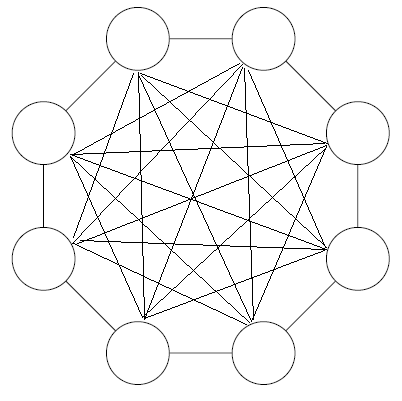
\includegraphics[scale=0.2]{image/Star.png}\label{fig:Star}}
\hspace{1mm}
\subfigure[]{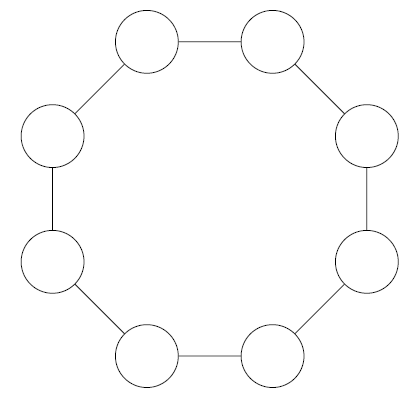
\includegraphics[scale=0.2]{image/Ring.png}\label{fig:Ring}}
\hspace{1mm}
\subfigure[]{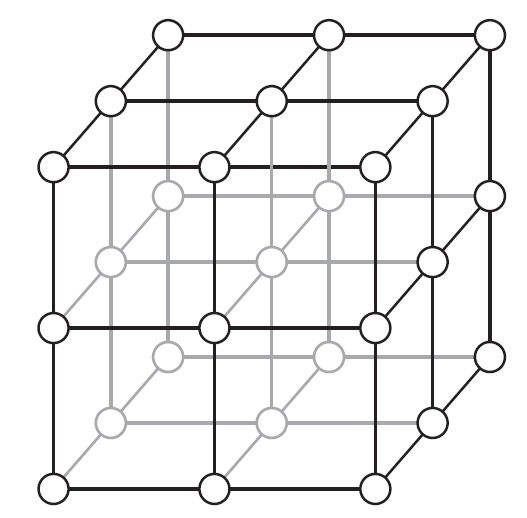
\includegraphics[scale=0.2]{image/vonneumann.png}\label{fig:vonneumann}}
\caption{Standard PSO communication topologies: (a) Star Topology used in $g_{best}$, (b) Ring Topology used in $l_{best}$ and (c) Von Neumann Topology.}
\label{fig:topologies}
\end{figure}

Figure \ref{fig:Star} presents the \emph{star} topology, in which the particles share information globally through a fully-connected structure. In this case, the information is quickly spread within the swarm and allows a quick convergence of the swarm. This topology is also known as global topology or $g_{best}$. Figure \ref{fig:Ring} presents the \emph{ring} topology, in which each particle is connected solely to $n$ neighbors. In this case, the information exchange mechanism allows a slower dissemination of information and helps to avoid local minima. The Ring topology is also known as local topology or $l_{best}$. The Von Neumann topology is depicted in Figure \ref{fig:vonneumann}. This is a balanced solution that consists in particles connected by a grid \cite{ClanPSO:Carvalho2009}.

The PSO execution occurs balancing the social learning and the individual learning of the individuals within the swarm. During each algorithm iteration, the particles move through the search space by updating their velocities and positions. There are several equations that can be used to update the velocity of the particles \cite{PSO:Clerc2002}. The most used equations to update the velocity and the position of particles are presented in the equations (\ref{eq:PSO_velocity}) and (\ref{eq:PSO_position}), respectively.
\begin{equation}\label{eq:PSO_velocity}
\vec v(t+1) = \omega \vec v(t) + r_1c_1[\vec p(t) - \vec x(t)] + r_2c_2[\vec n(t) - \vec x(t)],
\end{equation}

\begin{equation}\label{eq:PSO_position}
\vec x(t+1) = \vec x(t) + \vec v(t),
\end{equation}
in which $\vec v(t)$ is the velocity of particle in time step $t$, $r_1$ and $r_2$ are random numbers selected by using an uniform probability density distribution in the interval $[0,1]$. $c_1$ is the cognitive acceleration coefficient, $c_2$ is the social acceleration coefficient and $\omega$ is the inertial factor. $r_1c_1[\vec p(t) - \vec x(t)]$ is the cognitive component, which attracts the particle to its own best position ($\vec p(t)$), and $r_2c_2[\vec n(t) - \vec x(t)]$ is the social component, which attracts the particle to the best position found by its own neighborhood ($\vec n(t)$).

In the beginning of the algorithm execution, position ($\vec x(t)$) and velocity ($\vec v(t)$) of particles are attributed randomly. In the state-of-art \cite{PSO:Shi} \cite{PSO:Bratton2007}, the standard values of parameters $c_1$, $c_2$ are equal (2.05) and the inertial factor($\omega$) linearly decreasing from $\omega_{max} = 0.9$ to $\omega_{min} = 0.4$, along the iterations. Equation (\ref{eq:PSO_inertial}) calculates the linear decrement of the inertial factor \cite{PSO:Shi}.
\begin{equation}\label{eq:PSO_inertial}
\omega = \omega_{max} - \Bigl[(\omega_{max} - \omega_{min})\frac{g(t)}{g_{end}}\Bigr],
\end{equation}
where $g(t)$ is current iteration and $g_{end}$ is total number of iterations. The inertial factor optimizes the exploration-exploitation tradeoff. This decrement is done to allow the swarm to have a higher exploration ability in the initial iterations, and a higher exploitation capability in final iterations, when probably the swarm has found a good region of the search space to exploit.

\subsection{Pseudocode of the PSO Algorithm}
The pseudocode of the PSO algorithm is shown in Algorithm \ref{alg:PSO}. One can observe that the PSO algorithm, basically, consists on particle movement in search space (lines 6 and 7) and the update process of the cognitive (lines 9 and 10) and social memories (lines 12 and 13, respectively). The adaptation of inertial factor (line 16) allows the algorithm to regulate the exploitation-exploration tradeoff.

\begin{algorithm}[!h]
    Initialize particles of swarm\;
    Initialize inertial factor\;
    Initialize social and cognitive memory\;
    \While {the stop criterion is not achieved}{
        \For {each particle}{
            Update the velocity according to Equation (\ref{eq:PSO_velocity})\;
            Update the position according to Equation (\ref{eq:PSO_position})\;
            Evaluate the position using the objective function of problem\;
            \If{current position is better than cognitive memory}
            {
                Update the cognitive memory\;
            }
            \If{current position is better than social memory}
            {
                Update the social memory\;
            }
        }
        Update inertial factor according to Equation (\ref{eq:PSO_inertial})\;
    }
    \Return the social memory.
    \caption{Pseudocode of the PSO algorithm.}
    \label{alg:PSO}
\end{algorithm}

\section{Adaptive Particle Swarm Optimization - APSO}\label{sec:APSO}
Zhan \emph{et al.} proposed the Adaptive Particle Swarm Optimization (APSO) in 2009 \cite{APSO:Zhan2009}. This variation of PSO was proposed to solve two inefficiencies of the standard PSO algorithm: low convergence velocity and incapability to avoid local minima. The Adaptive PSO aims to achieve these goals with a systematic adaptation of the parameters and the use of an elitist learning strategy.

Basically, the APSO consists in a loop with the following steps: (\emph{i}) evaluate and estimate the distribution of particles in search space through the metric proposed by authors, called evolutionary factor; (\emph{ii}) classify the evolutionary state of the swarm; (\emph{iii}) determinate the acceleration coefficients based on the evolutionary state (improving the convergence velocity); (\emph{iv}) maintain the diversity with elitist learning strategy; and, (\emph{v}) adapt the inertial factor, increasing the efficiency of the search process.

\subsection{Estimation of Evolutionary Factor}
One needs to estimate the evolutionary factor in order to control the adaptation process of the APSO. To accomplish this, it is necessary to evaluate the distribution of the particles in the search space along the iterations. One needs to calculate the average Euclidian distance of each particle to the other particles of the swarm. The average distance ($d_i$) between particle $i$ and the rest of the swarm is evaluated by Equation (\ref{eq:APSO_distance}).
\begin{equation}\label{eq:APSO_distance}
d_i = \frac{1}{N-1}\sum_{j=1,j\neq i}^{N}\sqrt{\sum_{k=1}^{D}(x_i^k - x_j^k)},
\end{equation}
in which $N$ is the number of particles in the swarm and $D$ is the number of dimensions.

Then, the evolutionary factor ($f_{evol}$) is calculated according to Equation (\ref{eq:APSO_factor}).
\begin{equation}\label{eq:APSO_factor}
f_{evol} = \frac{d_g - d_{min}}{d_{max} - d_{min}} \ \  \in \ \ [0,1],
\end{equation}
in which $d_g$ is the average distance between the best particle of the swarm and the rest of the swarm, $d_{min}$ and $d_{max}$ are the smallest and the biggest average distance among all particles, respectively. To avoid $d_{min} = d_{max}$, it is necessary to have at least three particles in the population.

$f_{evol}$ is a number in the interval $[0,1]$. If the swarm is close to the best particle, then the evolutionary factor is close to $0$. On the other hand, if the particles of swarm are completely spread over the search space, then the evolutionary factor is close to $1$.

\subsection{Classification of Evolutionary State}
The original proposal of the APSO algorithm classifies the swarm in an evolutionary state using fuzzy rules. The evolutionary state is chosen at each iteration based on the membership function with higher value. Figure \ref{fig:factor_APSO} presents the four membership functions for the four evolutionary states: Convergence, Exploitation, Exploration and Jumping out.

\begin{figure}[!h]
\centering
 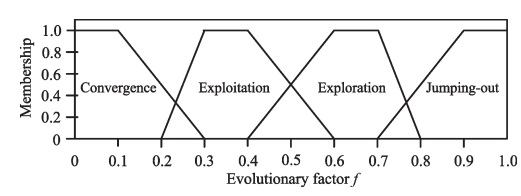
\includegraphics[width=0.65\textwidth]{image/factor}
 \caption{\small{Fuzzy membership functions for the APSO algorithm.}}
 \label{fig:factor_APSO}
\end{figure}

\emph{Convergence State}: it occurs when the value of the evolutionary factor is minimal and the particles are very close of the best particle. This means that the algorithm found a good region of the search space and then it is currently refining the solutions. We calculate the fuzzy value of this state according to Equation (\ref{eq:s_convergence}).
\begin{equation}
S_{convergence}(f_{evol}) = \begin{cases}
1,                 & \mbox{if $0.0 \leq f_{evol} \leq 0.1$}, \\
-5f_{evol} + 1.5,  & \mbox{if $0.1    < f_{evol} \leq 0.3$}, \\
0,                 & \mbox{if $0.3    < f_{evol} \leq 1.0$}.
\end{cases}
\label{eq:s_convergence}
\end{equation}

\emph{Exploitation State}: it occurs when the value of the evolutionary factor is shrunk and the particles are near to the best particle, it indicates that the swarm found a good region of the search space. The membership function of this state is defined according to Equation (\ref{eq:s_exploitation}).
\begin{equation}
S_{exploitation}(f_{evol}) = \begin{cases}
0,                &\mbox{if $ 0.0 \leq f_{evol} \leq 0.2 $}, \\
10f_{evol} - 2,   &\mbox{if $ 0.2 <    f_{evol} \leq 0.3 $}, \\
1,                &\mbox{if $ 0.3 <    f_{evol} \leq 0.4 $}, \\
-5f_{evol} + 3,   &\mbox{if $ 0.4 <    f_{evol} \leq 0.6 $}, \\
0,                &\mbox{if $ 0.6 <    f_{evol} \leq 1.0 $}.
\end{cases}
\label{eq:s_exploitation}
\end{equation}

\emph{Exploration State}: it occurs when the value of the evolutionary factor is medium to large and the particles have a medium or large distant of the best particle. In this case, the algorithm is trying to find a good region of the search space. We calculate the fuzzy value of this state according to Equation (\ref{eq:s_exploration}).
\begin{equation}
S_{exploration}(f_{evol}) = \begin{cases}
0,                &\mbox{if $ 0.0 \leq f_{evol}  \leq 0.4 $}, \\
5f_{evol} - 2,    &\mbox{if $ 0.4   <  f_{evol}  \leq 0.6 $}, \\
1,                &\mbox{if $ 0.6   <  f_{evol}  \leq 0.7 $}, \\
-10f_{evol} + 8,  &\mbox{if $ 0.7   <  f_{evol}  \leq 0.8 $},  \\
0,                &\mbox{if $ 0.8   <  f_{evol}  \leq 1.0 $}.
\end{cases}
\label{eq:s_exploration}
\end{equation}

\emph{Jumping out State}: it occurs when the evolutionary factor presents large values. This means that the APSO is jumping out of a local optimum to a new region, in other words, the globally best particle is distinctively away from the cluster of the swarm. The membership function of this state is defined according to Equation (\ref{eq:s_jumpingout}).
\begin{equation}
S_{jumping_out}(f_{evol}) = \begin{cases}
0,                  &\mbox{if $ 0.0 \leq f_{evol} \leq 0.7 $}, \\
5f_{evol} - 3.5,    &\mbox{if $ 0.7    < f_{evol} \leq 0.9 $}, \\
1,                  &\mbox{if $ 0.9    < f_{evol} \leq 1.0 $}.
\end{cases}
\label{eq:s_jumpingout}
\end{equation}

\subsection{Adaptation of Acceleration Coefficients}
The next step is to update the acceleration coefficients $c_1$ and $c_2$, which are initialized with values equal to 2.0 and are updated according to the current value of $f_{evol}$. The rules to update the coefficients are depicted in Table \ref{tab:apso_strategies}.

\begin{table}[!ht]
\caption{Strategies for the control of acceleration coefficients $c_1$ and $c_2$.}
\centering
\begin{tabular}{c c c}
\hline
Evolutionary State  &   $c_{1}$               &  $c_{2}$ \\
\hline
Convergence    & Increase slightly     & Increase slightly \\
Exploitation   & Increase slightly     & Decrease slightly \\
Exploration    & Increase              & Decrease \\
Jumping out    & Decrease              & Increase  \\
\hline
\end{tabular}
\label{tab:apso_strategies}
\end{table}

In the \emph{Convergence} state, the $c_1$ value is slightly increased and the $c_2$ value slightly is increased. In this state, the swarm is located at a minima, and, hence, the influence of social coefficient should be prioritized to guide other particles to this region. Thus, the value of $c_2$ should be increased. On the other hand, the value of the cognitive coefficient should be decreased to guarantee the swarm to converge faster. The consequence of this strategy is a premature saturation of the cognitive and the social coefficients to their lower and upper bounds, respectively. Thus, the swarm will strongly be attracted by the current best region, causing premature convergence, which is unsuitable if the current best region is just a local optimum. To avoid this, both $c_1$ and $c_2$ are slightly increased.

In the \emph{Exploitation} state, the $c_1$ value is slightly increased and the $c_2$ value is slightly decreased. In the Exploitation state, each particle uses local information and the swarm form groups in potential local optimal regions, that were identified by the historical best position of each particle. Hence, $c_1$ is slowly increased and maintains a relatively large value to predominate the search and exploitation around the respective cognitive memories. Probably, the social memory is still not present in the global optimal region. Therefore, decreasing $c_2$ slowly can avoid the lock in local optimal. Furthermore, an exploitation state in more likely to occur after an exploration state and before a convergence state. Hence, changing directions for $c_1$ and $c_2$ should be slightly altered from the exploration state to the convergence state \cite{APSO:Zhan2009}.

In the \emph{Exploration} state, the $c_1$ value is increased and the $c_2$ value is decreased. In this state, is essential the swarm should explore so many optima search regions as possible. hence, increasing $c_1$ and decreasing $c_2$ can help each particle explores individually and achieve its own historical best positions. In this case, we aim to avoid that the current best particle of swarm get stucked in a local optimum.

In the \emph{Jumping out} state, the $c_1$ value is decreased and the $c_2$ value is increased. When the best particle is jumping out of the local optimum toward a better optimum, it is very likely to be far away from the core of the swarm in presented in the Convergence state. As soon as this new region is found by a particle, which becomes the (possibly new) guide, others should follow it and achieve this new region as fast as possible. To guarantee this behavior of the swarm, a large $c_2$ value together with a relatively small $c_1$ value is more indicated.

The incremented or decremented value of acceleration coefficients is called acceleration rate ($\delta$). In the APSO algorithm, this value is a random number uniformly generated  among the interval [0.05, 0.1]. The term ``slightly'' found in strategies of Convergence and Exploitation states, implies in the use of acceleration rate equal to 50\% ($\delta \cdot 0.5$).

In the coefficients adaptation process, they can achieve huge or small values, generating unstable moments in search process. To solve this, the authors of APSO proposed a normalization of acceleration coefficient values. The lower and upper boundaries of acceleration coefficients are $c_{min} = 1.5$ and $c_{max} = 2.5$, respectively. If the sum of $c_1$ and $c_2$ is larger than 4.0, the acceleration coefficients should be normalized according to Equation (\ref{eq:APSO_normalized}).
\begin{equation}\label{eq:APSO_normalized}
c_i = \frac{c_i(c_{min} + c_{max})}{c_1 + c_2}, \ \ i = 1,2.
\end{equation}

\subsection{Elitist Learning Strategy}
The third step is the application of a operator in order to generate diversity. The authors named it as Learning Strategy using Elitism and this mechanism aims to improve the global search capability of the algorithm. It was first proposed to be applied just in the best particle during the Convergence state, generating the Jumping out state.

The reason for this operator is because the best particle does not have exemplars to follow. As a means to improve its own, a perturbation was developed to help the best particle to push itself out of a local minima to a potential better search region. If the new region is better, then the rest of swarm will follow quickly the leader in order to converge to this new search region.

This is a type of greedy local search applied only in one dimension ($d$) of the current best particle ($\vec n_i (t)$) of the swarm aiming to allow this particle to escape from a local optimum. All the dimensions have the same probability to be chosen. The Gaussian mutation is generated according to Equation (\ref{eq:APSO_elitism}).
\begin{equation} \label{eq:APSO_elitism}
\vec n_i(t+1) = \vec n_i(t) + (X_{max}^d - X_{min}^d)G(\mu,\sigma^2),
\end{equation}
in which $(X_{max}^d, X_{min}^d)$ are the boundaries of search space, $G(\mu,\sigma^2)$ is a random number generated by Gaussian distribution with a zero mean $\mu$ and standard deviation $\sigma$, which is called the elitist learning rate. The authors suggested that $\sigma$ be linearly decreased with the iterations number and is calculated by Equation (\ref{eq:apso_sigma}).
\begin{equation} \label{eq:apso_sigma}
\sigma = \sigma_{max} - \Bigl[(\sigma_{max} - \sigma_{min})\frac{g(t)}{g_{final}}\Bigr],
\end{equation}
in which ($\sigma_{max},\sigma_{min}$) are the boundaries of $\sigma$, $g(t)$ is the current iterations and $g_{final}$ is the total number of iterations. In empirical tests, Zhan \emph{et al.} proposed to use $\sigma$ = 1.0 in the beginning of the simulations, with the objective to escape from a local optimum and decrease it to $\sigma$ = 0.1 at the end of the simulation, to refine the found solutions.

The position of the best particle is updated only if the new position found by the operator is better than the previous one. Otherwise, the new position will replace the worst particle in the swarm.

\subsection{Adaptation of Inertial Factor}
In the last step, the inertial factor $\omega$ is updated using equation (\ref{eq:APSO_inertial}) in order to auto-adapt the exploration-exploitation ability of the swarm.
\begin{equation}\label{eq:APSO_inertial}
\omega(f_{evol}) = \frac{1}{1 + 1.5e^{-2.6f_{evol}}} \ \ \in \ \ [0.4;0.9], \ \ \forall f_{evol} \ \ \in \ \ [0,1].
\end{equation}

\subsection{Pseudocode of the APSO Algorithm}
The pseudocode of the APSO algorithm is shown in Algorithm \ref{alg:APSO}. The APSO algorithm has the same main steps that are found in the PSO algorithm. However, one can observe the adaptation of parameters (acceleration coefficients and inertial factor) in the lines 3 to 20. In lines 3 to 6, one can observe the steps needed to estimate the evolutionary factor. The classification of evolutionary state of swarm can be observed in lines 7 and 8. In the lines 9 and 10, one can observe the adaptation of acceleration coefficients. In line 11, the adaptation of inertial factor is executed. In the lines 12 to 19, one can observe the execution of elitist learning strategy.

\begin{algorithm}[!h]
    Initialize particles of swarm\;
    \While {the stop criterion is not achieved}{
        \For {each particle}{
            Calculate the average distance according to Equation (\ref{eq:APSO_distance})\;
        }
        Calculate the evolutionary factor according to Equation (\ref{eq:APSO_factor})\;
        Calculate the membership function according to Equations (\ref{eq:s_convergence}), (\ref{eq:s_exploitation}), (\ref{eq:s_exploration}) and (\ref{eq:s_jumpingout})\;
        Classify the swarm in the evolutionary state\;
        Adapt the acceleration coefficients according to Table \ref{tab:apso_strategies}\;
        Normalize the acceleration coefficients according to Equation (\ref{eq:APSO_normalized})\;
        Update the inertial factor according to Equation (\ref{eq:APSO_inertial})\;
        \If{classified on \emph{Convergence} state}
        {
            Generate a new position using the Equations (\ref{eq:APSO_elitism}) and (\ref{eq:apso_sigma})\;
            \If{new position is better than the best cognitive memory}
            {
                Update the position and cognitive memory of the best particle\;
            }
            \Else
            {
                Update the position and cognitive memory of the worst particle\;
            }
        }
        \For {each particle}
        {
            Update the social memory in neighborhood\;
            Update the velocity according to Equation (\ref{eq:PSO_velocity})\;
            Update the position according to Equation (\ref{eq:PSO_position})\;
            Evaluate the position using the objective function of problem\;
            \If{current position is better than cognitive memory}
            {
                Update the cognitive memory\;
            }
            \If{current position is better than social memory}
            {
                Update the social memory\;
            }
        }
    }
    \Return the social memory.
    \caption{Pseudocode of the APSO algorithm.}
    \label{alg:APSO}
\end{algorithm}

\section{Clan Particle Swarm Optimization - ClanPSO}\label{sec:ClanPSO}
Clans are groups of individuals united by a kinship based on a lineage, for example. Some clans stipulate a common ancestor to become the leader of the clan, and every individual of the clan will be guided by this leader. Incorporating this characteristic, a topology was proposed for improving the PSO algorithm performance, the Clan Particle Swarm Optimization \cite{ClanPSO:Carvalho2008}. This topology consists in a set of clan, where each clan is sub-swarm and uses a fully-connected structure to share information. The structure presented in Figure \ref{fig:clans} is an example with four clans (A, B, C and D) of five particles.
\begin{figure}[!h]
\centering
 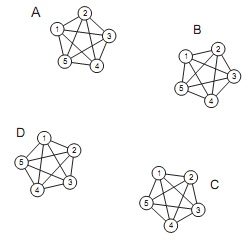
\includegraphics[width=0.35\textwidth]{image/Clan}
 \caption{\small{Example of division of the population in sub-swarms.}}
 \label{fig:clans}
\end{figure}

Other approach was proposed that enables the migration of particles among clans and some improvements were reached for some benchmark function \cite{ClanPSO:Carvalho2009}. However, there are some problems in this case, such as possibility of empty clans.

In this algorithm, the population size is divided according to the number of particle per clan ($N_{pc}$). For each iteration, each one of clans performs a search using a classical PSO and selects the particle that had achieved the best position of the entire clan. This particle is called the leader and this process of marking is called delegation. After the definition of all leaders, we form a new swarm with only the leaders of clans and we execute the PSO algorithm just with the leaders. This process is called conference of leaders. We can observe in more details these execution steps of the ClanPSO algorithm.

\subsection{Delegation of Leaders}
Is similarly to complex social behavior, with several clans with various leaders. The definition of a leader in clan is a marking process the best particle in the swarm, for example in Figure \ref{fig:leaders}. The delegation process is based in the global information exchange mechanism inside each clan, which uses $\vec{n_{best}}$ information to delegate the leader.
\begin{figure}[!h]
\centering
 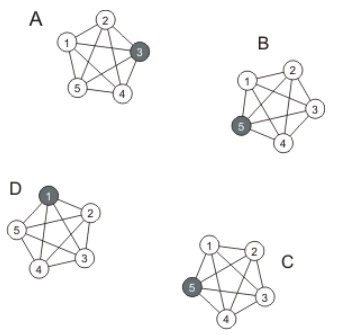
\includegraphics[width=0.35\textwidth]{image/Leaders}
 \caption{\small{Example of definition of clans leaders (A, B, C and D).}}
 \label{fig:leaders}
\end{figure}

\subsection{Conference of Leaders}
After the delegation, the leaders need to adjust their positions based on the best leader. This second step consists in execution of PSO only with the leaders, and is called conference of leaders. The conference can be performed using either the star (observe Figure \ref{fig:conference_star}) or ring (observe Figure \ref{fig:conference_ring}) topology.

\begin{figure}[!h]
\centering
\subfigure[]{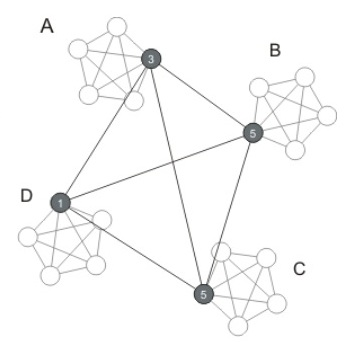
\includegraphics[scale=0.5]{image/conference_star}\label{fig:conference_star}}
\hspace{1mm}
\subfigure[]{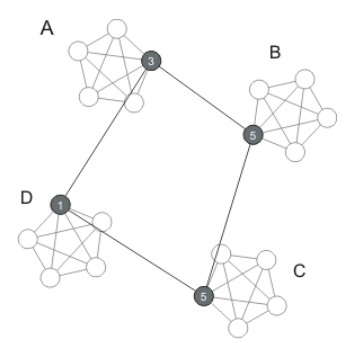
\includegraphics[scale=0.5]{image/conference_ring}\label{fig:conference_ring}}
\caption{Types of conference in the ClanPSO: (a) global conference and (b) local conference.}
\label{fig:conference}
\end{figure}

The topology to be used depends on the kind of problem to be solved. When the star topology is used, the information is spread faster between leaders through of global information share, guaranteeing a better exploitation ability. When is used ring topology, the communication between leaders is slower, thus the algorithm has great exploration ability. The convergence velocity is smaller than in star topology, but the quality of the solutions are often better.

\subsection{The Information shared within the clans}
After the leaders conference, the leaders will return to its respective clans and the new information acquired in the process will be widely used inside each clan to adjust the other particles. Indirectly, allows that all other particles be guided by the best position found within the entire topology. Through indirect communication, a foreign leader does not directly influence another clan, and then preserves the  exploration capacity of clans.

\subsection{Pseudocode of the ClanPSO Algorithm}
The pseudocode of the ClanPSO algorithm is shown in Algorithm \ref{alg:ClanPSO}. In the lines 4 to 14, one can observe the PSO execution within of each clan. In lines 17 to 28, one can observe the leaders conference. We can observe the leaders delegation in the lines 5 and 16, and still the line 5, the return of information from the leaders conference.

\begin{algorithm}[!h]
    Initialize the particles with random positions and velocities\;
    Group the particles in clans with global topology\;
    \While {the stop criterion is not achieved}{
        \For {each clan}{
            Find the best particle and mark as leader\;
            Update the velocity according to Equation (\ref{eq:PSO_velocity})\;
            Update the position according to Equation (\ref{eq:PSO_position})\;
            Evaluate the position using objective function of the problem\;
            \If{new position is better than cognitive memory}
            {
                Update cognitive memory\;
            }
            \If{new position is better than social memory}
            {
                Update social memory\;
            }
        }
        Add clan leader in the leaders list\;
        \For {each leader particle of the list}
        {
            Find the best particle\;
            Update the velocity according to Equation (\ref{eq:PSO_velocity})\;
            Update the position according to Equation (\ref{eq:PSO_position})\;
            Evaluate the position using objective function of the problem\;
            \If{new position is better}
            {
                Update cognitive memory\;
            }
            \If{new position is better than social memory}
            {
                Update social memory\;
            }
        }
    }
    \Return the social memory.
    \caption{Pseudocode of the ClanPSO algorithm.}
    \label{alg:ClanPSO}
\end{algorithm}

\section{Clan Adaptive Particle Swarm Optimization - ClanAPSO}\label{sec:ClanAPSO}
The Clan Adaptive Particle Swarm Optimization (ClanAPSO) was developed in 2011 \cite{ClanAPSO:Pontes2011}. This algorithm was proposed by aggregation of the process of systematic adaptation of parameters with a search strategy of multi-swarm. This technique was inspired in the clans topology presents in the ClanPSO algorithm combined to the concepts of parameters adaptation and elitist strategy found in the APSO algorithm.

The ClanAPSO algorithm presents an adaptation process in each swarm in a multi swarm system, this allows that sub-swarms can perform different types of search by iteration of the algorithm, \textit{i.e.} it is possible to perform exploitation and exploration search simultaneously in distinct regions of the search space. The concept of clans is interesting because it allows to identify local leaders of groups of particles (clans) and carry out the information share between clans indirectly. The indirect communication between clans promotes improvement the search process because it is a distributed process of spreading information.

There are two versions of the ClanAPSO algorithm. The original version \cite{ClanAPSO:Pontes2011} executes the APSO algorithm within the clans and also execute the APSO in the conference of leaders. The proposed second version \cite{ClanAPSO:Vitorino2011} also includes the adaptation capability within the clans, but in the leaders conference is running the PSO algorithm.

\subsection{Pseudocode of the ClanAPSO Algorithm}
The simplified pseudocode of the ClanAPSO algorithm is shown in Algorithm \ref{alg:ClanAPSO}. In the lines 3 to 6, the APSO execution within of each clan is presented. In the lines 7 and 8, one can observe the conference of leaders, where they can be executed by the APSO algorithm or the PSO algorithm. We can observe the leaders delegation in the line 5.

\begin{algorithm}[!h]
    Initialize the particles with random positions and velocities\;
    \While {the stop criterion is not achieved}{
        \For {each clan}{
            Execute APSO within the clans\;
            Delegate leader\;
        }
        Create conference of leaders\;
        Execute APSO (or PSO) with the leaders\;
    }
    \Return the best particle.
    \caption{Pseudocode of the ClanAPSO algorithm.}
    \label{alg:ClanAPSO}
\end{algorithm}

\section{Artificial Bee Colony - ABC}\label{sec:ABC}
The ABC algorithm was proposed by Karaboga in 2005 \cite{ABC:Karaboga2005}. ABC is an algorithm of search and optimization modeled by the behavior of honey bees \cite{ABC:Karaboga2006} \cite{ABC:Karaboga2007} \cite{ABC:Karaboga2009a} \cite{ABC:Karaboga2009b} \cite{ABC:Ziarati2011}. The bee colony is one of the natural societies with the most specialized social divisions. In the simplified model assumed by the ABC, the bee colony is composed by three types of bees: employed bees, onlookers and scouts. Initially, the swarm is divided in equal parts of employed bees and onlookers bees. The employed bees are those that go to the food source explored by herself, there is a food source to each employed bee. The bees that wait in the hive and decide to exploit a food source depending on the information shared by the employed bees are called onlooker bees. The onlookers are guided bees. When the food source does not improve its quality, the associated employed bee is now scout bee, which is responsible to find a new valuable food source. We will call them guide bees in exploration mode.

Basically, the steps of the algorithm executed in each iteration are: (\emph{i}) the employed bees explore its respective food sources; (\emph{ii}) it is determined the quality of food sources, which are shared to onlooker bees; (\emph{iii}) the onlooker bees choose a food source and help to explore the food source selected; (\emph{iv}) if the food source does not improve, the associated employed bee becomes scout bee. The scout bees find randomly new source food and determine its quality. In the end of each iteration, the best food source is saved until the end of the algorithm execution.

A food source represents a potential solution for the problem to be solved. The nectar quantity of a food source determines the solution quality of that food source. The onlooker bees choose the best food source using the selection method by roulette wheel.

The scout bees are explorers of the hive. They do not follow orientations to search food source, then this type of bees aims to find new food sources. The quality of these food source is not relevant (the most of cases is medium or low). However, in some cases, the scout bees find good food sources, that were unknown. The low search cost makes this mechanism of maintain diversity an attractive option.

We can observe that the ABC algorithm has exploitation-exploration tradeoff because the employed and onlookers bees has exploitation capability and scout bees has exploration capability.

\subsection{Quality of Food Source}
The quality of food source is calculated based on objective function value of problem according to Equation (\ref{eq:abc_quality}) \cite{ABC:Murgan2012}.
\begin{equation}
Q[\vec{x}(t)] = \begin{cases}
\frac{1}{f[\vec{x}(t)]+1}, &\mbox{if $ f[\vec{x}(t)] \geq 0 $}, \\
1+abs{f[\vec{x}(t)]+1},    &\mbox{if $ f[\vec{x}(t)] < 0 $}, \\
\end{cases}
\label{eq:abc_quality}
\end{equation}
in which $\vec{x}(t)$ is food source position, $abs$ is value of absolute function, $Q[\vec{x}(t)]$ is the quantity of food source nectar presents in position $\vec{x}(t)$ and $f[\vec{x}(t)]$ is the value of the objective function in position $\vec{x}(t)$.

\subsection{Update of Food Source}
In the algorithm, the search space of the problem is $D$-dimensional. The number of the employed bees and the onlookers are the same and for every food source, there is only one employed bee per food source. In other words, the size of employed and onlooker bees is equal $SN$ (the number of food sources). Each $i$th source food associated to the employed bee will be optimized according to Equation (\ref{eq:ABC_employed}).
\begin{equation}\label{eq:ABC_employed}
v_{id} = x_{id} + r_{id}(x_{id} - x_{kd}),
\end{equation}
in which $d = 1,2,...,D$ is the number of dimensions, $r_{id}$ is a random generalized real number within the range [-1,1], $k = 1,2,...,SN$ is a randomly selected index number in the colony, it has to be different from the $i$. The new solution ($v_{id}$) is compared with the previous one ($x_{id}$), and the better one should be stored.

\subsection{Choose of Food Source by Onlookers Bees}
Next, the onlooker bee needs to select one of the food sources explored by the employed bees. The probability for each food source to be selected by the onlooker bee is:
\begin{equation}\label{eq:ABC_probability}
p_i = \frac{fit_i}{\sum_{j}^{SN}fit_j},
\end{equation}
in which $p_i$ is the probability to select the food source $i$, which is proportional to the quality of the food source, $fit_i$ is the fitness of the position $x_{id}$. Each onlooker bee searchers for a new solution in the selected food source by using Equation (\ref{eq:ABC_employed}).

\subsection{Stagnation of Food Source}
At each loop, the food source are evaluated and if the fitness of a source does not improve after a predetermined number of steps (called \textit{MaxTrial}), then it is abandoned. The employed bee associated with it becomes a scout and replaces the food source with a new one, through the random search given by Equation (\ref{eq:ABC_scout}).
\begin{equation}\label{eq:ABC_scout}
x_{id} =  x_d^{min} + r(x_d^{max} - x_d^{min}).
\end{equation}
in which $r$ is random number selected in range [0,1], and $x_d^{max}$ and $x_d^{min}$ are lower and upper borders in the $d^{th}$ dimension of the search space.

\subsection{Pseudocode of the ABC Algorithm}
The pseudocode of the ABC algorithm is shown in Algorithm \ref{alg:ABC}. In the pseudocode, we can observe the employed bees movement in lines 3 to 13. The probability used to selection of employed bees by onlooker bees can be observed in the line 16. Then, the onlooker bees movement can be observed in lines 18 to 28. If some food source does not improve, so the employed bee becomes a scout bee. This movement can be visualized in lines 29 to 35.
\begin{algorithm}[!h]
    Initialize the food sources in random positions\;
    \While {the stop criterion is not achieved}{
        \For {each employed bee}{
            Determine a different position randomly\;
            Update the position according to Equation (\ref{eq:ABC_employed})\;
            Evaluate the position using the objective function of problem\;
            \If{the new position is better}
            {
                Update the position of associated food source\;
            }
            \Else
            {
                Increase the stagnation counter of food source\;
            }
            Calculate the quality of new food source position according to Equation (\ref{eq:abc_quality})\;
        }
        \For {each employed bee}
        {
            Calculate the probability od roulette wheel selection using the Equation (\ref{eq:ABC_probability})\;
        }
        \For {each onlooker bee}
        {
            Determine two different positions chosen by roulette\;
            Update the position according to Equation (\ref{eq:ABC_employed})\;
            Evaluate the position using the objective function of problem\;
            \If{the new position is better}
            {
                Update the position of associated food source\;
            }
            \Else
            {
                Increase the stagnation counter of food source\;
            }
        }
        \For{each employed bee}
        {
            \If{stagnation counter achieved the threshold}
            {
                Generate a new position of associated food source randomly\;
                Restart the stagnation counter of associated food source\;
            }
        }
    }
    \Return the best food source.
    \caption{Pseudocode of the ABC algorithm.}
    \label{alg:ABC}
\end{algorithm}

\section{Fish School Search - FSS}\label{sec:FSS}
The Fish School Search (FSS) is a computational intelligence technique inspired in social behavior of schools of fish developed by Bastos-Filho and Lima-Neto in 2007 \cite{FSS:Bastos-Filho2008} \cite{FSS:BastosFilho2009}. It was conceived to solve search problems and was based in the gregarious behavior present in some fish species, with the objective to improve the survivability of the entire group through the mutual protection and synergy to perform collective tasks \cite{FSS:Lins2012}.

In the FSS algorithm, the search space, called aquarium, is limited region of objective function, the population is called school of fish and each fish has a weight. The weight of the fish represents the success of search process. Each position in the search space represents a possible solution of the problem.

During the execution, the operators of the algorithm are executed sequentially by updating the positions and weights of each fish. The FSS algorithm has four operators: individual movement (responsible by local search), feeding (indicator of success of search process), collective-instinctive movement (generates the displacement of school of fish) and collective-volitive movement (controls the exploitation-exploration granularity).

\subsection{Individual Movement Operator}
Initially, the fish try to find food and for this, the fish realize individual movements in the search space. The individual movement is executed by each fish in the school ($S$) in the beginning of each iteration.  Each fish chooses a new position in its neighborhood and then, this new position is evaluated using the objective function of problem. The individual movement operator is determined according to Equation (\ref{eq:FSS_individual}) for each dimension.
\begin{equation}\label{eq:FSS_individual}
v_{id}(t) = x_{id}(t) + rand[-1,1] \cdot step_{ind},
\end{equation}
in which $\vec v_i(t)$ is the candidate position of fish $i$, $\vec x_i(t)$ is the current position of the fish $i$, $rand[-1,1]$ is a random number generated by an uniform distribution in the range [-1,1] and $d$ is a number of dimensions. The $step_{ind}$ is a percentage of search space amplitude in dimension determined.

The $step_{ind}$ decreases linearly along the iterations according to Equation (\ref{eq:FSS_stepInd}), so the exploitation capability increases during search process.
\begin{equation}\label{eq:FSS_stepInd}
step_{ind} = step_{ind\_initial} - \Bigl[(step_{ind\_initial} - step_{ind\_end})\frac{g(t)}{g_{end}}\Bigr],
\end{equation}
in which $step_{ind\_initial}$ is the individual step in the beginning of the algorithm execution, $step_{ind\_end}$ is the individual step in the final of the algorithm execution, $g(t)$ is the current iteration and $g_{end}$ is the total number of iterations.

After the calculation of the candidate position, the movement just occurs if the new position has better fitness than the old one.

\subsection{Feeding Operator}
The fish weight can grow or decrease, depending on its success or failure in the search for food, when the individual movement is realized. In each iteration, the fish weight is updated according to Equation (\ref{eq:FSS_feed}).
\begin{equation}\label{eq:FSS_feed}
W_i(t+1) = W_i(t) + \frac{\Delta f_i}{max(\Delta f)},
\end{equation}
in which $W_i(t)$ is the weight of the fish, $\Delta f_i$  is the difference between the fitness value of new position ($f[\vec x(t+1)]$) and the fitness value of the current position for each fish ($f[\vec x(t)]$), this value is calculated according to Equation (\ref{eq:FSS_Delta}). The $max(\Delta f)$ is the maximum value of these differences in the current iteration.
\begin{equation}\label{eq:FSS_Delta}
\Delta f = f[\vec x(t+1)] - f[\vec x(t)].
\end{equation}

In order to avoid a explosion state of the weight values, the algorithm has a maximum value, called weight scale ($W_{scale}$), that is defined to limit the weight of fish. The initial weight for each fish is equal to $\frac{W_{scale}}{2}$.
\subsection{Collective-Instinctive Movement Operator}
After the individual movement, the fish are evaluated and is observed if were successful in the food search or not. Therefore, the school should move based in the successful fish, \textit{i.e.} is a global movement in direction, probably, to richer region of food.

The position of all the fish are updated with this movement according to Equation (\ref{eq:FSS_instinctive}).
\begin{equation}\label{eq:FSS_instinctive}
\vec x_i(t+1) = \vec x_i(t) + \frac{\sum_{i=1}^{N}\Delta \vec x_{ind_i} \Delta f_i}{\sum_{i=1}^{N}\Delta f_i},
\end{equation}
in which $\Delta \vec x_{ind_i}$ is the displacement of the fish $i$ due to the individual movement in the FSS cycle. One must observe that $\Delta \vec x_{ind_i} = 0$ for fish that did not execute the individual movement \cite{FSS:Lins2012}.

\subsection{Collective-Volitive Movement Operator}\label{sse:FSS_volitive}
After the other two movements, the school of fish executes the collective-volitive movement. This movement is global able to make the school fish expand or contract. If the fish school search has been successful, \textit{i.e.} its weight is increasing, the radius of the school should contract to better exploitation capability; if not, it should expand, allowing better exploration capability. Thus, this operator increases the capacity to auto-regulate the exploration-exploitation granularity \cite{FSS:Lins2012}.

To realize the school dilation or contraction in each fish position is necessary the school centroid, which can be evaluated by using the Equation (\ref{eq:FSS_centroid}).
\begin{equation}\label{eq:FSS_centroid}
\vec B(t) = \frac{\sum_{i=1}^{N}\vec x_iW_i(t)}{\sum_{i=1}^{N}W_i(t)}.
\end{equation}

The movement is executed according to Equation (\ref{eq:FSS_volitive}). To the fish school expansion, we use signal `$+$' and to the fish school contraction, we use signal `$-$'.
\begin{equation}\label{eq:FSS_volitive}
\vec x_i(t+1) = \vec x_i(t) \pm step_{vol}r_1 \frac{\vec x_i(t) - \vec B(t)}{d(\vec x_i(t) ,\vec B(t))},
\end{equation}
in which $step_{vol}$ is called volitive step, $r_1$ is a random number generated by uniform probability density function in the range [0,1]. $d(\vec x_i(t) ,\vec B(t))$ calculates the euclidian distance between the particle $i$ and the centroid.

The $step_{vol}$ value decreases linearly along the iterations of the algorithm according to Equation (\ref{eq:FSS_stepVol}). Thus, the algorithm initializes with an exploration ability and changes to an exploitation mode. The parameter value is defined as a percentage of the search space range and is bounded by two parameters ($step_{vol\_initial}$ and $step_{vol\_end}$).
\begin{equation}\label{eq:FSS_stepVol}
step_{vol}(t) = step_{vol\_initial} - \Bigl[(step_{vol\_initial} - step_{vol\_end}) \frac{g(t)}{g_{end}}\Bigr],
\end{equation}
in which $g(t)$ is the current iteration and $g_{end}$ is the total number of iterations. Usually, $step_{vol} = step_{ind}$.

After the update of all the fish, is necessary to evaluate the school fish with objective function of problem, thus they will be prepared for the next iteration.

\subsection{Pseudocode of the FSS Algorithm}
The pseudocode of the FSS algorithm is shown in Algorithm \ref{alg:FSS}. In the lines 3 to 9, we can observe the individual movement that each fish realizes. In the line 17, one can observe the collective-instinctive movement and in the lines 19 to 26, the collective-volitive movement. In the lines 5 and 27, one can observe the evaluation of objective function of problem. %Thus, to comparison of algorithms performance should realize the adjusts suitable of parameter setup.

\begin{algorithm}[!h]
    Initialize the population in random positions\;
    \While {the stop criterion is not achieved}{
        \For {each fish}{
            Execute individual movement according to Equation (\ref{eq:FSS_individual})\;
            Evaluate position using the objective function of problem\;
            \If{new position is better}
            {
                Update the fish memory\;
            }
        }
        Update the individual step according to Equation (\ref{eq:FSS_stepInd})\;
        Calculate the population weight before to adjust it\;
        \For {each fish}
        {
            Adjust the weight according to Equation (\ref{eq:FSS_feed})\;
        }
        Calculate the population weight after of the adjust of the all the fish\;
        \For{each fish}
        {
            Execute the instinctive movement according to Equation (\ref{eq:FSS_instinctive})\;
        }
        Calculate the centroid of the swarm according to Equation (\ref{eq:FSS_centroid})\;
        \For{each fish}
        {
            \If{swarm increased its weight}
            {
                Execute volitive movement of contraction according to Equation (\ref{eq:FSS_volitive})\;
            }
            \Else
            {
                Execute volitive movement of dispersion according to Equation (\ref{eq:FSS_volitive})\;
            }
            Evaluate the position using objective function of problem\;
            \If{new position is better}
            {
                Update the fish memory\;
            }
        }
        Update the volitive step according to Equation (\ref{eq:FSS_stepVol})\;
    }
    \Return the best memory of school of fish.
    \caption{Pseudocode of the FSS algorithm.}
    \label{alg:FSS}
\end{algorithm}

\section{Discussion about the Swarm Intelligence Algorithms}
This chapter described the main swarm intelligence algorithms that were essential to development of proposed algorithm in this dissertation.

\emph{Particle Swarm Optimization - PSO}: this is standard version of the algorithm. It is the most known swarm intelligence algorithm, very simple and easy deployment. This algorithm is very used in unimodal problems due to its convergence ability, but is not recommended  in multimodal problems because the algorithm has limitations to maintain diversity of swarm. Other approaches were developed  to solve these limitations \cite{PSO:Clerc99} \cite{PSO:Clerc2002} as new communications topologies \cite{ClanPSO:Carvalho2008} \cite{ClanPSO:Carvalho2009} \cite{ClanAPSO:Pontes2011} \cite{MultiPSO:Bastos2008}.

\emph{Adaptive Particle Swarm Optimization - APSO}: was proposed to solve two limitations of original PSO, the low convergence velocity and incapability to escape of local minimum. This approach presents a systematic scheme to update the PSO parameters based on an evolutionary factor, that is calculated through distribution of particles in search space. This scheme allows a better control of convergence velocity and ability to escape of local minimum.

\emph{Clan Particle Swarm Optimization - ClanPSO}: a new topology for PSO algorithm compound by particle clans which communicate in conference to share information. The exchange of information indirectly between the clans can offer improved performance of the algorithm, avoiding premature convergence. However, setting the number of particles per clans and clan may depend on the problem.

\emph{Clan Adaptive Particle Swarm Optimization - ClanAPSO}: was introduced the APSO algorithm concepts in each clan. It was used another independent APSO (or PSO) to perform the conference of leaders.  Thus, each clan adapt itself independently and, as a consequence, the algorithm will avoid to exploit excessively the same spot or converge prematurely.

\emph{Artificial Bee Colony - ABC}: was inspired in honey bees behavior and has the ability to explore richer food sources with the onlooker (guided bees) and employed (guide bees in exploitation mode) bees. This exploitation ability is controlled with stagnation counter and the algorithm maintains the diversity of bee colony with the scout bees (guide bees in exploration mode).

\emph{Fish School Search - FSS}: was inspired in school of fish behavior and has two global movements. The first movement moves the school in direction the fish that achieved the best results. The second movement regulates the search granularity, allowing the contraction or expansion of school. Due the presence of two fitness evaluation, this algorithm is slower than other approaches, such as PSO.

Table \ref{tab:Param_Algorithm} shows the number of parameters of each algorithm that need to setup. Some parameters present standard values, but the researcher can change it.

\begin{table}[!h]
\caption{\small{The number of parameters of each algorithm.}}
\centering
\begin{tabular}{>{\centering\arraybackslash}m{1in} | >{\centering\arraybackslash}m{1in} | >{\centering\arraybackslash}m{2in}}
\hline
\textbf{Algorithm}  & \textbf{Number of Parameters} & \textbf{Parameters}\\
\hline
\textbf{PSO}      &   5  & $N$, $c_1$, $c_2$, $\omega_{min}$, $\omega_{max}$\\
\textbf{APSO}     &   5  & $N$, $c_1$, $c_2$, $\omega_{min}$, $\omega_{max}$\\
\textbf{ClanPSO}  &   6  & $N$, $c_1$, $c_2$, $\omega_{min}$, $\omega_{max}$, $N_{pc}$\\
\textbf{ClanAPSO} &   6  & $N$, $c_1$, $c_2$, $\omega_{min}$, $\omega_{max}$, $N_{pc}$\\
\textbf{ABC}      &   2  & $2 \cdot SN$, $MaxTrial$\\
\textbf{FSS}      &   6  & $S$, $W_{scale}$, $step_{vol\_initial}$, $step_{vol\_final}$, $step_{ind\_initial}$, $step_{ind\_final}$ \\
\hline
\end{tabular}
\label{tab:Param_Algorithm}
\end{table}

This dissertation proposes to combine two well known swarm intelligence algorithms: the APSO algorithm and the ABC algorithm. The proposed algorithm has a operator based on bees behavior (the ABC algorithm) to generate diversity for Particle Swarm Optimization with adaptive behavior.
\pagebreak

  \chapter{Methodology}\label{cap:methodology}

%Nessa dissertação, propõe-se uma metodologia para a análise de risco em projetos de software, a partir de dados históricos de registros de riscos, por meio da utilização de redes neurais artificiais. Para desenvolver essa metodologia, primeiramente necessita-se de uma base de dados extensa e real de riscos em projetos de software. No entanto, há uma dificuldade em encontrar publicamente bases de dados representativas e confiáveis. Uma base de dados de risco chamada PERIL \cite{kendrick2003identifying} mostrou atender as necessidades básicas para essa pesquisa, além de já estar totalmente classificada (mais detalhes na Seção \ref{sec:perildataset}). Nesse estudo, precisa-se de uma base de dados extensa de registros de riscos oriundos de diversos projetos espalhados pelo mundo e em diversos períodos de tempo, com o objetivo de mostrar evidências de quais são os principais modos de falha em projetos e um padrão para explorar respostas aos riscos.
In this dissertation, it is proposed a methodology for risk analysis in software projects, from historical database of risk registers, through the use of artificial neural networks. To develop this methodology, first it is needed an extensive and real database of risks in software projects. However, there is a difficulty in finding publicly bases of representative and reliable data. A database called risk PERIL \cite{kendrick2003identifying} showed  to meet basic needs for this research, in addition to already be fully classified (more details in Section \ref{sec:perildataset}). This study requires an extensive database of risk registers from various projects around the world and in different time periods in order to show evidence of which are the main modes of failure in projects and a standard for explore risk responses.

%Segundo, é necessário realizar o pré-processamento dos dados para que as variáveis de entradas sejam transformadas, normalizadas e selecionadas para o estudo. Terceiro, avaliar o desempenho das ferramentas de estado da arte quanto ao erro de previsão: Simulação de Monte Carlo e Análise PERT.
Second, it is necessary to perform data preprocessing for input variables to be converted into numeric, standardized and selected for the study. Third, evaluate the performance of state of the art tools about forecast error, Monte Carlo simulation and PERT Analysis.

%Quarto, implementar cada modelo de previsão para que pudéssemos selecionar o melhor modelo em redes neurais artificiais: Perceptron de Múltiplas Camadas, Máquinas de Vetor de Suporte, Redes de Função de Base Radial e o Sistema de Inferência Adaptativo Neuro-Fuzzy. Alguns desses modelos selecionados apresentam alguns parâmetros e devido a diversidade de possíveis valores para cada parâmetro, necessita-se otimizar os parâmetros dos modelos. Nesse estudo, implementa-se uma variação da meta-heurística Otimização por Enxame de Partículas (PSO - \textit{Particle Swarm Optimization}) com coeficiente de constrição de Clerk \cite{engelbrecht2007computational} para realizar a tarefa de otimização dos parâmetros das RNAs. O espaço de busca do problema de otimização desses parâmetros é multi-dimensional, complexo e apresenta diversos mínimos locais. 
Fourth, implement each prediction model so we could select the best model in artificial neural networks: Multilayer Perceptron, Support Vector Machine, Radial Basis Function and the Adaptive Neuro-Fuzzy Inference System. Some of these selected models have some parameters and due to the diversity of possible values for each parameter, one needs to optimize the parameters of the models. This study implements a variation of meta-heuristic Particle Swarm Optimization (PSO) with a constriction coefficient of Clerk \cite{engelbrecht2007computational} to accomplish the task of optimizing the parameters of ANNs. The search space of the problem of optimization of these parameters is multi-dimensional, complex and has many local minima.

%Na Figura \ref{fig:method2}, observa-se um esquema ilustrando que um algoritmo de otimização executa os quatro modelos em suas diversas configurações paramétricas para que seja possível eleger o modelo mais eficiente para a base de dados adotada.
In Figure \ref{fig:method2}, it is observed a schematic showing that an optimization algorithm performs the four models in its various parametric settings so you can choose the most efficient model for the chosen database.

\begin{figure}[h]
	\centering
	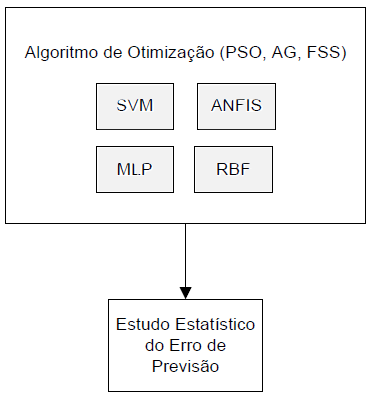
\includegraphics[width=.45\textwidth]{image/MetodologiaDissertacao2.png}
	%\caption{Esquema de Seleção da Melhor Rede Neural Artificial}
	\caption{Schema for selection of best ANN}
	\label{fig:method2}
\end{figure}

%Quinto, um teste de validação dos resultados é realizado para verificar se os modelos baseados em redes neurais artificiais apresentam menor erro que os modelos de estado da arte em análise de riscos: Simulação de Monte Carlo, Análise PERT, Modelo de Regressão Linear Múltipla, Modelo de Regressão em Árvore. Os dois últimos modelos de regressão linear foram considerados como linha de base, por serem modelos mais simples, já que realizam a regressão linear. Os dois últimos modelos foram implementados e também são avaliados quanto ao erro na previsão.
Fifth, a validation test of outcomes is carried out to check whether models based on artificial neural networks have lower error than state of the art models in risk analysis: Monte Carlo Simulation, PERT Analysis, Multiple Linear Regression, Regression Tree Model. The first two models have been implemented and are also evaluated for error in prediction. The last two, were considered baseline for being simpler models since they perform linear regression.

%A seleção do melhor modelo é feita em termos da precisão na estimativa dos impactos dos riscos. É difícil obter uma métrica representativa da precisão de um modelo. No entanto, Engelbrecht \cite{engelbrecht2007computational} e Saxena \cite{saxena2012software} sugerem que a Raiz do Erro Médio Quadrático(REMQ) é uma medida conveniente e aplicável para a maioria dos problemas. A precisão, nesse caso, significa o grau de proximidade de uma saída calculada para a esperada. A REMQ é representada pela Equação \ref{eq:RMSE}:
The selection of the best model is made in terms of accuracy in estimating the impacts of risks. It is difficult to obtain a representative measure of the accuracy of a model. However, Engelbrecht \cite{engelbrecht2007computational} and Saxena \cite{saxena2012software} suggest that the Root Mean Square Error (RMSE) is a convenient measure applicable to most problems. Accuracy in this case means the degree of closeness calculated for an expected output. RMSE is represented by Equation \ref{eq:RMSE}:

\begin{equation}\label{eq:RMSE}
    REMQ= \sqrt[2]{\frac{1}{n}\sum_{i=1}^{n} (e_i)^2},
\end{equation}

%onde $e_i=f_i - y_i$, $f_i$ é o resultado calculado, $y_i$ é o resultado esperado e $n$ é o número de tuplas de dados.
where $e_i=f_i - y_i$, $f_i$ is the calculated outcome, $y_i$ is the expected outcome and $n$ is the number of data pairs.

%Todas as técnicas estudadas nesse trabalho estimam a saída para o impacto de riscos, a REMQ é calculada trinta vezes para cada abordagem e um Teste Estatístico de Wilcoxon Não-pareado \cite{siegel1956nonparametric} pode ser necessário para determinar qual é uma abordagem mais precisa para a base de dados (nesse estudo, o PERIL). O Teste de Wilcoxon não-pareado é utilizado porque não há evidências que as amostras sejam oriundas de uma população normalmente distribuída, como também não há relação de ordem nos valores pertencentes às amostras.
The eight selected techniques have predicted the outcome to risk impacts. Root Mean Square Error is calculated thirty times for each method. Nevertheless, a Non-paired Wilcoxon Test \cite{siegel1956nonparametric} may be necessary to assert which is a more efficient approach to fit dataset (e.g. PERIL). Non-paired Wilcoxon Test is used because there were no evidence that the samples came from a normally distributed population, either there were no relation between outcomes from different samples.

%A validação cruzada \cite{amari1996statistical} é utilizada para evitar a ocorrência de \textit{overfitting} ou \textit{underfitting} durante o treinamento das RNA's. Nesse caso, um treinamento com parada prematura é utilizado para identificar o início do \textit{overfitting}, já que esse método tem provado ser capaz de melhorar a capacidade de generalização da RNA em comparação com o treinamento exaustivo \cite{haykin-1994} \cite{engelbrecht2007computational} \cite{amari1996new}. Portanto, o método de validação cruzada é utilizado para cada abordagem, excluindo a Simulação de Monte Carlo e Análise PERT, para promover maior capacidade de generalização. Quando adotamos o uso da validação cruzada, significa que necessitamos particionar a base de dados em três partes: conjunto de treinamento, conjunto de validação cruzada e conjunto de testes. O conjunto de treinamento é utilizado na fase de treinamento das RNA's, momento em que o aprendizado ocorre. O conjunto de validação cruzada é processado ao mesmo tempo, com o conjunto de treinamento e determina a parada no treinamento. Já o conjunto de testes, é utilizado para produzir a métrica de precisão do modelo, o REMQ.
Furthermore, cross-validation \cite{amari1996statistical} must be used to avoid the occurrence of overfitting or underfitting of data training. In this situation \textit{early stopping} training is used to identify the beginning of overfitting because this method has been proved to be capable of improving the generalization performance of the ANN over exhaustive training \cite{haykin1994neural} \cite{engelbrecht2007computational} \cite{amari1996new}. Therefore, cross-validation method is used for each alternative, excluding Monte Carlo Simulation and PERT Analysis, to promote higher generalization performance. When cross-validation is adopted, it means that it is needed to partition the database into three disjoint groups: training, cross-validation and test subset. Training set is used in training phase the RNA's, at which learning takes place. Cross-validation subset is processed simultaneously with training subset and determine the stop in network training since test subset is used to obtain accuracy of the model, RMSE.

%Por fim, a previsão do impacto do risco e a definição de um intervalo de confiança para uma amostra do conjunto de treinamento são obtidas utilizando o modelo de previsão mais preciso após os testes de validação. É necessário um intervalo de confiança da previsão para que os gerentes de projetos e analistas de risco possam estabelecer o nível de confiança de acordo com a sua necessidade. Afinal de contas, esse é o resultado que eles esperam.
Finally, risk impact estimation and establishment of a confidence interval for a sample of the training set are obtained using the most accurate prediction model after validation tests. It is necessary to define a confidence interval of prediction for project managers and risk analysts establish the confidence level according to their needs. After all, this is the result they expect.

%A Figura \ref{fig:method} apresenta um fluxograma com a metodologia estabelecida para esse estudo. O procedimento inicia-se com a seleção da base de dados que serve como conjunto de dados de entrada, nesse caso o PERIL, e finaliza com a atividade "Definição do Intervalo de Confiança". Todas as atividades são executadas sequencialmente, exceto as atividades "Avaliação dos Modelos de Estado da Arte" e "Seleção da Melhor Rede Neural Artificial" que são executados paralelamente.
Figure \ref{fig:method} presents a flowchart with the established methodology for this study. The procedure begins with the selection of the database that serves as a set of input data, in this case the PERIL, and ends with the activity "Definition of Confidence Interval". All activities are executed sequentially, except activities "Evaluation of Models of State of the Art" and "Best Selection of Artificial Neural Network" that run in parallel. 

\begin{figure}[h]
	\centering
	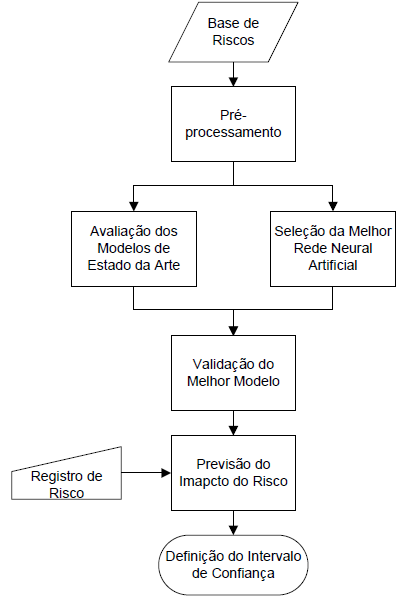
\includegraphics[width=.45\textwidth]{image/MetodologiaDissertacao.png}
%	\caption{Fluxograma do estudo realizado}
	\caption{Flowchart of performed study}
	\label{fig:method}
\end{figure}

\section{PERIL Database}
\label{sec:perildataset}

A better risk management starts identifying potential problems, asserted here as risk factors. The adoption of available methods like: reviewing learned lessons, brainstorming, interviews and specialized judgment are suposed to be relative efficient alternatives, otherwise in most of situations it involves high costs. A low cost, extensive and accessible proposal is to utilize Project Experience Risk Information Library (PERIL) database \cite{kendrick2003identifying}. PERIL database provides information and experience of other project risk management.
%Um melhor gerenciamento de riscos inicia com a identificação de problemas potenciais, atribuído como fatores de risco. A adoção dos métodos disponíveis como: revisar lições aprendidas, \textit{brainstorming}, entrevistas e opinião especializada são alternativas relativamente eficientes, no entanto, na maioria das situações elas envolvem alto custo. Uma proposta de baixo custo, extensiva e acessível é utilizar a base de dados \textit{Project Experience Risk Information Library}(PERIL) \cite{kendrick2003identifying}. A base de dados PERIL provê informações e experiências de outras gestões de risco de projetos.

For more than a decade, in Risk Management Workshops, Kendrick have collected anonymous data from hundred of project leaders dealing with their past project problems. He has compiled this data in the PERIL database, which summarizes both a description of what went wrong and the amount of impact it had on each project. The dataset provides a sobering perspective on what future projects may face and is valuable in helping to identify at least some of what might otherwise be invisible risks or black swans \cite{kendrick2003identifying}.
%Por mais de uma década, durante \textit{Workshops} de Gerenciamento de Riscos, Kendrick coletou dados anônimos de centenas de líderes de projetos lidando com seus problemas em projetos passados. Ele compilou essas informações na base de dados PERIL, que sumariza tanto uma descrição do que houve de errado quanto o impacto que ele teve em cada projeto. A base provê uma perspectiva preocupante do que projetos futuros podem encarar e é valiosa na ajuda para a identificação do que pelo menos poderiam ter sido riscos invisíveis ou \textit{black swans} \cite{kendrick2003identifying}.

According to Kendrick, in projects, the identified risks can be classified as "known", those anticipated during planning, or "unknown" further identified during project execution. The purpose of this dataset is to provide a framework to identify risks, in such a way to increase the number of "known", and decrease the amount of "unknown" risks \cite{kendrick2003identifying}.
%Segundo Kendrick, em projetos, os riscos identificados podem ser classificados como "conhecidos", aqueles antecipados durante o planejamento, ou "desconhecidos", identificados futuramente durante a execução do projeto. O propósito dessa base de dados é prover um \textit{framework} para identificar riscos, de modo a aumentar o número de "conhecidos" e diminuir o número de "desconhecidos" \cite{kendrick2003identifying}.

Some characteristics of PERIL are: 
\begin{itemize}
\item the data are not relational, they contain only a small fraction of the tens of thousands projects undertaken by the project leaders from whom they were collected;
\item they present bias, the information was not collected randomly;
\item they represent only the most significant risks;
\item they are worldwide, with a majority from the Americas;
\item they do not identify opportunities; 
\item they contain six hundred and forty nine registers, whose relative impact is based on the number of weeks delayed the project schedule;
\item typical project had a planned duration between six months and one year;
\item typical staffing was rarely larger than about twenty people.
\end{itemize}
%Algumas características da PERIL são:
%\begin{itemize}
%\item Os dados não estão relacionados, eles representam somente uma pequena fração de dezenas de milhares de projetos realizados pelos líderes de projetos, cujos riscos foram coletados;
%\item Apresentam viés, a informação não foi coletada aleatoriamente;
%\item Representam somente os riscos mais significativos;
%\item São de todo o mundo, com a maioria nas Américas;
%\item Não identificam oportunidades; 
%\item Contém seis centos e quarenta e nove registros, cujo impacto relativo é baseado no número de semanas de atraso no cronograma;
%\item Projetos comuns tiveram um cronograma inicialmente planejado entre seis meses e um ano;
%\item Tamanho da equipe raramente foi maior que vinte pessoas.
%\end{itemize}

Risk registers are categorized as scope, schedule and resource. Scope is decomposed in change and defect subcategories. Schedule is decomposed in dependency, estimative and delay subcategories. Resources is decomposed in money, outsourcing and people subcategories. One benefit of PERIL is that the author contemplates "black swans": risks with large impact, difficult to predict and with rare occurrence \cite{taleb2001fooled}. 
%Os registros de risco são categorizados em escopo, cronograma e recurso. O escopo é decomposto nas subcategorias mudança e defeito. O cronograma é decomposto em dependência, estimativa e atraso. Os recursos são decompostos em dinheiro, \textit{outsourcing} e pessoas. Um benefício da PERIL é que o autor contempla "\textit{black swans}": riscos com grande impacto, difíceis de prever e com ocorrência rara \cite{taleb2001fooled}.

Kendrick chose to normalize all the quantitative data using only time impact, measured in weeks of project slippage. This tactic made sense in light of today's obsession with meeting deadlines, and it was an easy choice because by far the most prevalent serious impact reported in this data was deadline slip. Focusing on time is also appropriate because among the project triple constraints of scope, time ans cost, time is the only one that's completely out of our control - when it's gone, it's gone \cite{KEND2003BOOK}.
%Kendrick decidiu padronizar o impacto usando como métrica o tempo, medido em semanas de atraso no projeto. Essa tática faz sentido à luz da obsessão de hoje por cumprimento de prazos e foi uma escolha fácil, pois, de longe, o impacto mais sério relatado nesses dados foi o atraso no prazo. Focar-se em tempo também é apropriado porque entre as restrições triplas de projeto - escopo, tempo e custo -, tempo é o único é completamente fora de nosso controle. Afinal, quando se vai, se foi \cite{KEND2003BOOK}.

%\begin{table}[h]
%\caption{Impacto total de projetos pelas causas-raiz de categorias e subcategorias %\cite{KEND2003BOOK}}\label{tab:peril_pareto} \centering
%\begin{tabular}{|l|c|c|c|c|}
% \hline
% Subcat. & & & Impacto & Impacto \\
% Causas-raiz & Definição & Casos & Cumul. & Médio \\
% \hline
%  Escopo: & Revisão no escopo &  &  &  \\
%  Mudanças & durante o projeto & 177 & 1460 & 8,2 \\
% \hline
%  Recurso: &  &  &  &  \\
%  Pessoas & Problemas de relacionamento interno & 123 & 706 & 5,7 \\
% \hline
%  Escopo: & Falha em alcançar  &  &  &  \\
%  Defeito & requisitos de entrega & 93 & 654 & 7,0 \\
% \hline
%  Cronograma: & Atraso devido a fatores &  &  &  \\
%  Atrasos & sob o controle do projeto & 102 & 509 & 5,0 \\
% \hline
%  Cronograma: & Durações inadequadas alocadas &  &  &  \\
%  Estimativas & para atividades do projeto & 49 & 370 & 7,6 \\
% \hline
%  Recurso: &  &  &  &  \\
%  \textit{Outsourcing} & Problemas de relacionamento externo & 47 & 316 & 6,7 \\
% \hline
%  Cronograma: & Atraso no projeto devido &  &  &  \\
%  Dependências & a fatores externos & 41 & 262 & 6,4 \\
% \hline
%  Escopo: &  &  &  &  \\
%  Mudanças & Financiamento insuficiente & 17 & 228 & 13,4 \\
% \hline
%\end{tabular}
%\end{table}
\begin{table}[h]
\caption{Total project impact by root-cause categories and subcategories \cite{KEND2003BOOK}}\label{tab:peril_pareto} \centering
\begin{tabular}{|l|c|c|c|c|}
 \hline
 Root-Cause & & &Cumulative &Average \\
 Subcategories &Definition &Cases &Impact(weeks) &Impact(weeks) \\
 \hline
  Scope: & Revision made to scope &  &  &  \\
  Changes & during the project & 177 & 1,460 & 8.2 \\
 \hline
  Resource: &  &  &  &  \\
  People & Issues arising from internal staffing & 123 & 706 & 5.7 \\
 \hline
  Scope: & Failure to meet deliverable &  &  &  \\
  Defects & requirements & 93 & 654 & 7.0 \\
 \hline
  Schedule: & Project slippage due to factors &  &  &  \\
  Delays & under the control of the project & 102 & 509 & 5.0 \\
 \hline
  Schedule: & Inadequate durations allocated &  &  &  \\
  Estimates & to project activities & 49 & 370 & 7.6 \\
 \hline
  Resource: &  &  &  &  \\
  Outsourcing & Issues arising from external staffing & 47 & 316 & 6.7 \\
 \hline
  Schedule: & Project slippage due to factors &  &  &  \\
  Dependencies & outside the project & 41 & 262 & 6.4 \\
 \hline
  Scope: &  &  &  &  \\
  Changes & Insufficient project funding & 17 & 228 & 13.4 \\
 \hline
\end{tabular}
\end{table}

%A Tabela \ref{tab:peril_pareto} apresenta o número de casos, o impacto cumulativo e médio em semanas para cada categoria e sub-categoria de causa-raiz, além do significado de cada subcategoria.
Table \ref{tab:peril_pareto} shows the number of cases, the cumulative and average impact in weeks for each category and sub-category of root cause, beyond the meaning of each subcategory.

%Uma desvantagem dessa base de dados é que ela somente contabiliza riscos que tiveram impacto negativo no projeto. As oportunidades não foram identificadas e analisadas nesse estudo. No entanto, um dos grandes benefícios é que o autor apresenta alguns riscos como \textit{black swans} \cite{KEND2003BOOK}, representando a idéia de riscos com amplo impacto, difíceis de prever e raros de ocorrer. Se o risco tiver impacto negativo é conhecido como catástrofe, ao passo que, se tiver impacto positivo é conhecido como recompensa.
A disadvantage of this database is that it only accounts for risks that negatively impact on the project. The opportunities were not identified and maximized in that study. However, A major benefit is that the author presents some risks as black swans \cite{KEND2003BOOK}: representing the idea of risks with broad impact, hard to predict and rare to occur. If the risk has negative impact, is known as a catastrophe, whereas, if you have positive impact, is known as a reward.

\subsection{Black Swans}

Calling some risks "black swans" has been popularized of late by the writings of Nassim Nicholas Taleb \cite{taleb2001fooled}. The notion of a "black swan" originated in Europe before there was much knowledge of the rest of the world. Because all the swans observed in Europe were white, a black swan was deemed impossible. It came as something of a shock when a species of black swans was later discovered in Australia. This realization gave rise to the metaphorical use of the term "black swan" to describe something erroneously believed to be impossible.
%Denominar alguns riscos como \textit{black swans} têm sido popularizado desde os textos de Nassim Nicholas Taleb \cite{taleb2001fooled}. A noção de \textit{black swan} originou-se na Europa antes de ser popularizada pelo Mundo. Já que todos os cisnes observados na Europa eram brancos, um cisne negro era considerado impossível de existir. Porém, foi como um choque quando uma espécie de cisne negro foi descoberta na Austrália. Esse fato deu origem ao uso metafórico do termo \textit{black swan} para descrever algo erroneamente acreditado ser impossível.

Taleb's concept of "black swan" is a large-impact, hard-to-predict, rare event. It is nonetheless applicable to project risk management. In projects, it is common for project leaders to discount major project risks because they are estimated to have extremely low probabilities. But these risks do occur - The PERIL database is full of them - and the severity of problems they cause means that ignoring them can be unwise. When these risks do occur, the same project managers who initially dismissed them come to perceive them as much more predictable - sometimes even inevitable \cite{KEND2003BOOK}.
%O conceito de Taleb acerca de \textit{black swan} é um evento raro, difícil de prever e de grande impacto. Mas não deixa de ser aplicável a gestão de risco do projeto. Nos projetos, é comum que os líderes de projeto para descontar principais riscos do projeto, porque eles são estimados para ter probabilidades extremamente baixas. No entanto, esses riscos ocorrem - a PERIL é cheia deles - e a severidade dos problemas que eles causam significa que ignorá-los pode ser imprudente. Quando esses riscos ocorrem, o mesmo gerente de projetos que inicialmente os negaram começam a percebê-los como muito mais previsíveis - às vezes até mesmo inevitáveis \cite{KEND2003BOOK}.

In PERIL database, there are 127 cases representing the most schedule slippage. As the database shows, these most damaging risks are not as rare as might be thought, and they need not be so difficult for project managers to predict if they get appropriate attention in the risk management process \cite{KEND2003BOOK}. In many situations, the most difficult task is to identify and estimate "black swans" due to its characteristic: emergent, unexpected, unpredictable and extreme impact events. Therefore, "black swans" also will be included in this study.
%Na PERIL, há 127 casos representando os maiores atrasos no cronograma. Como a base de dados mostra, estes riscos mais danosos não são tão raros quanto devem ser pensados, e não devem ser tão difíceis de ser previstos por gerentes se eles dedicarem a atenção apropriada para o processo de gerenciamento de riscos \cite{KEND2003BOOK}. Em muitas situações, a tarefa mais difícil é identificar e estimar \textit{black swans} devido a sua característica: emergente, inesperado, imprevisível e com alto impacto. Portanto, \textit{black swans} também são considerados nesse estudo.

\section{Data Preprocessing}
\label{sec:datapreprocessing}

PERIL contains nominal and numeric values. So, nominal variables were expressed through binary variables. In that point, it is used fifteen binaries variables to represent nine nominal variables. Second, impact which represents the real output, are integer numbers. It has been noticed that impact probability distribution function fits with log-normal, gamma functions. Therefore, it was done a gamma data normalization \cite{han2006data}. The selection of the most significant variables for the study was performed after the results of the analysis promoted by Random Forest algorithm proposed in Luís Torgo book \cite{torgo2003data}.
%PERIL contém valores nominais e numéricos, dessa forma variáveis nominais são expressas através de variáveis binárias. Nesse estudo, utilizam-se doze variáveis binárias para representar as variáveis nominais. O impacto que representa a saída real, são números inteiros. Foi observado que a função de distribuição de probabilidade do impacto ajusta-se às funções log-normal e gamma. Portanto, foi realizada uma normalização gamma \cite{han2006data}. A seleção das variáveis mais significativas para o estudo foi realizada após o resultado da análise promovida pelo algoritmo \textit{Random Forest} proposto no livro de Luís Torgo \cite{torgo2003data}.

Figure \ref{fig:input16} e \ref{fig:input712} introduced input variables in histograms. All data are binary values represented by bar graphs, that means the number of occurrences for each value interval. Figure \ref{fig:impacthistogram} presents gamma normalized real outcome from PERIL in a histogram. A shape of the distribution fitting function is also presented in a curve under the histogram.
%A Figura \ref{fig:input16} e \ref{fig:input712} apresentam os histogramas das variáveis de entrada. Todos os dados encontram-se binarizados como pode ser observado nos gráficos em barras, que contém o número de ocorrências para cada intervalo de valores. A Figura \ref{fig:impacthistogram} apresenta a saída normalizada pela função gamma para a PERIL num histograma. A forma da função de distribuição de probabilidade é exibida como uma curva sobre o histograma.

\begin{figure}[h]
  \vspace{-0.2cm}
  \centering
  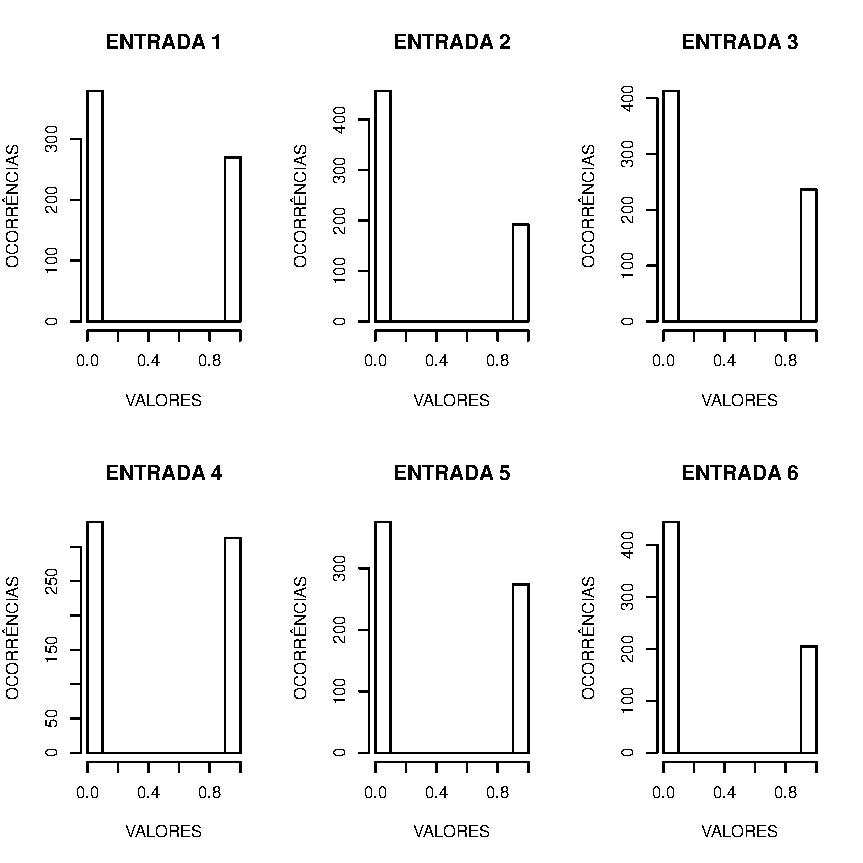
\includegraphics[width=0.7\columnwidth]{image/input1_6.pdf}
  \caption{First six input variables}
  \label{fig:input16}
\end{figure}
%\begin{figure}[h]
%  \vspace{-0.2cm}
%  \centering
%  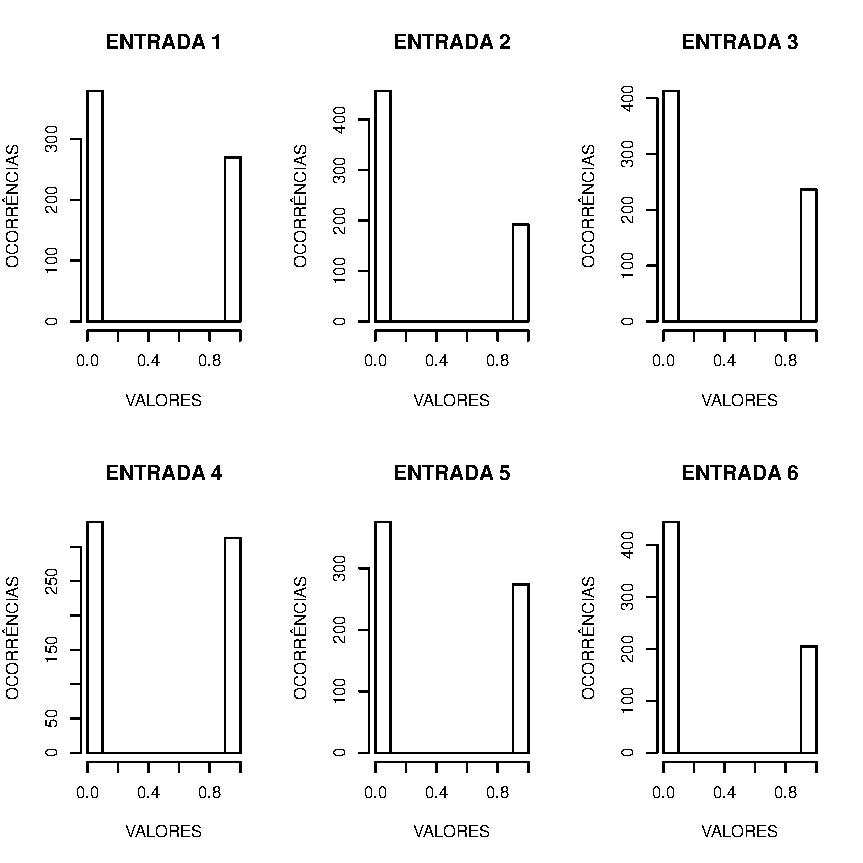
\includegraphics[width=0.7\columnwidth]{image/input1_6.pdf}
%  \caption{Primeiras seis variáveis de entrada}
%  \label{fig:input16}
%\end{figure}

\begin{figure}[h]
  \vspace{-0.2cm}
  \centering
  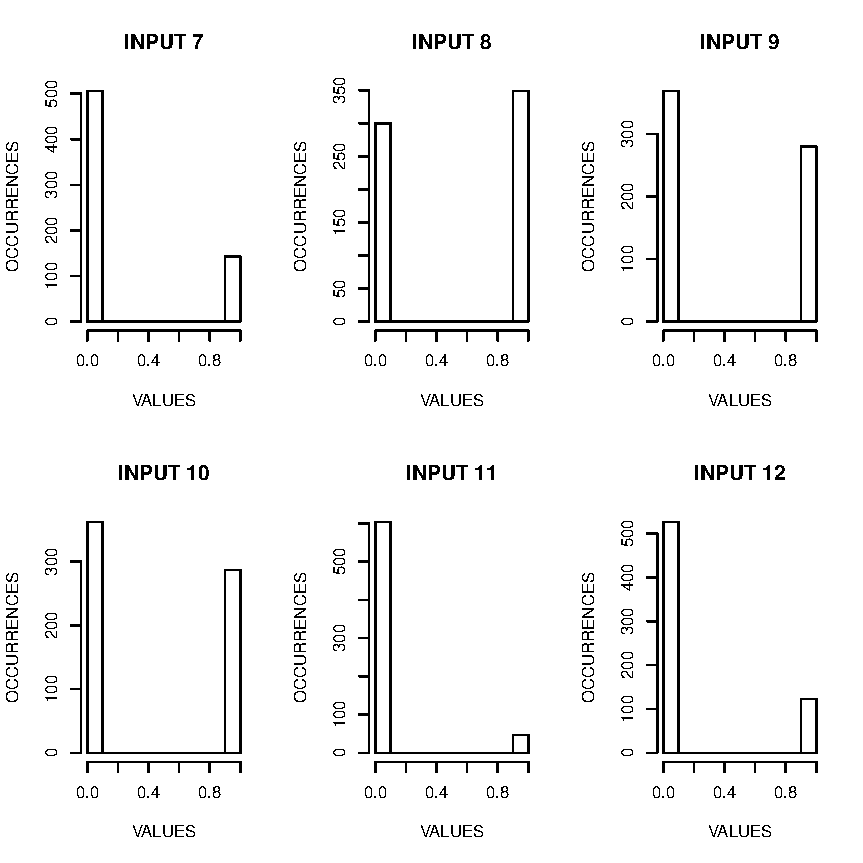
\includegraphics[width=0.7\columnwidth]{image/input7_12.pdf}
  \caption{Last six input variables}
  \label{fig:input712}
\end{figure}
%\begin{figure}[h]
%  \vspace{-0.2cm}
%  \centering
%  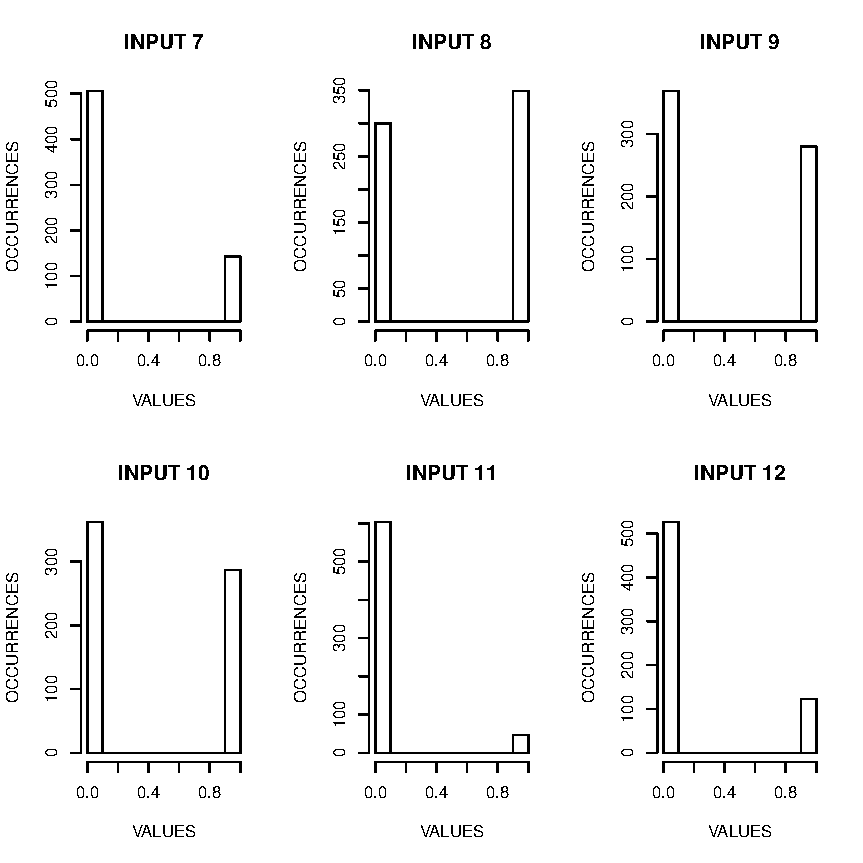
\includegraphics[width=0.7\columnwidth]{image/input7_12.pdf}
%  \caption{Últimas seis variáveis de entrada}
%  \label{fig:input712}
%\end{figure}

\begin{figure}[h]
  \vspace{-0.2cm}
  \centering
  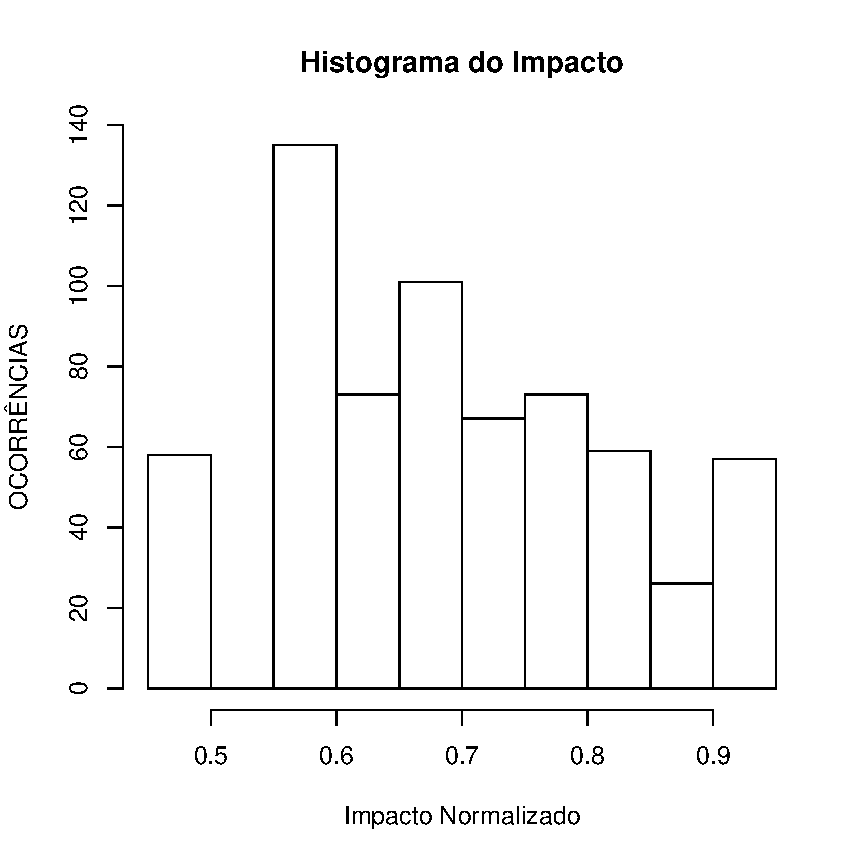
\includegraphics[width=0.5\columnwidth]{image/impact_histogram.pdf}
  \caption{Histogram of impact and shape of the distribution fitting function}
  \label{fig:impacthistogram}
\end{figure}
%\begin{figure}[h]
%  \vspace{-0.2cm}
%  \centering
%  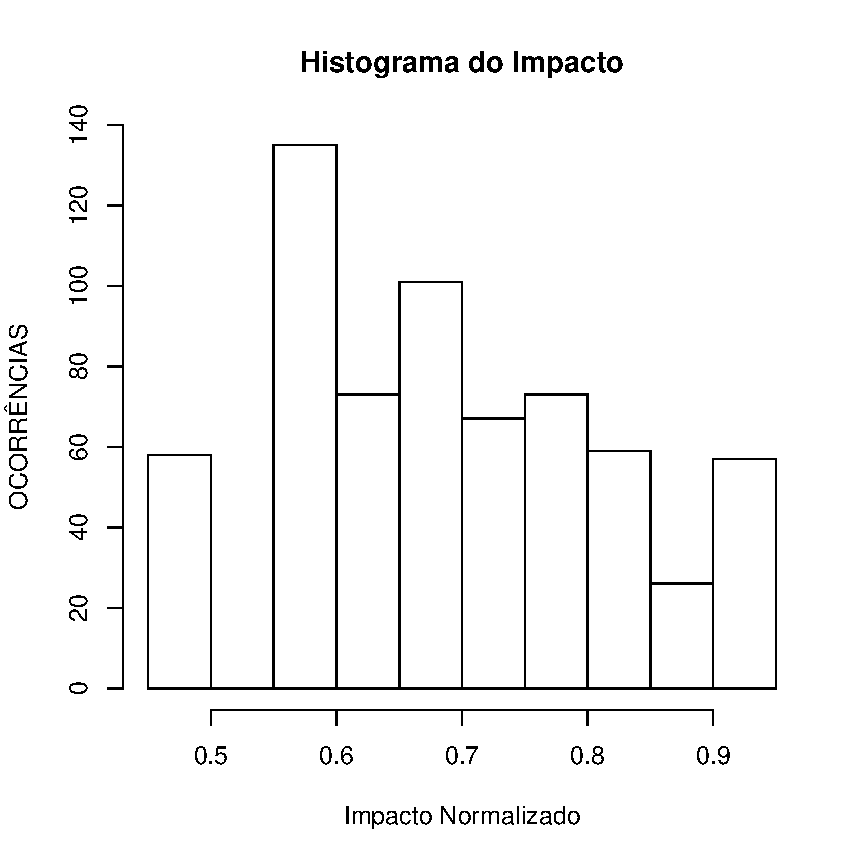
\includegraphics[width=0.5\columnwidth]{image/impact_histogram.pdf}
%  \caption{Histograma do impacto e forma da função de distribuição de ajuste}
%  \label{fig:impacthistogram}
%\end{figure}

For our purpose, PERIL was split into three disjoint subsets - training, cross-validation and test subsets, corresponding to fifty, twenty-five and twenty five percent of the dataset, respectively. \textit{Split-sample} cross-validation method was used for MLRM and RTM models. Whereas \textit{early stopping} and \textit{split-sample} cross-validation methods were combined and used for MLP, SVM, RBF and ANFIS training \cite{priddy2005artificial}.
%Para o nosso objetivo, PERIL foi dividida em três subconjuntos disjuntos - treinamento, validação cruzada e teste, correspondendo a cinquenta, vinte e cinco porcento e o restante da base de dados, respectivamente. O método de validação-cruzada com divisão de amostras foi utilizado tanto para o MRLM e o MRA quanto para o MLP, SVM, RBF e o ANFIS; sendo que para esses o método da parada prematura também foi utilizada no treinamento \cite{priddy2005artificial}.

\section{State of art models}
\label{sec:models}

%Nesta seção, são descritos as configurações adotadas para a experimentação dos modelos de estado da arte.
In this section, adopted configurations for experiments of state of art models are described.

\subsection{Monte Carlo Simulation}

MCS technique used the entire dataset in order to increase the performance prediction. It was filtered only the possible real outcomes to generate the calculated outcome. Towards this decision, we have reduced prediction issues and have improved its performance.
%A Simulação de Monte Carlo utilizou a base de dados inteira com o objetivo de aumentar o desempenho do modelo durante a previsão. Além disso, foram filtradas somente as saídas possíveis para uma dada entrada para que uma nova saída pudesse ser calculada. Através desse método, o desempenho da estimativa do impacto dos riscos foi melhorado.

\subsection{PERT Analysis}

%A Análise PERT também utilizou a base de dados inteira e somente as saídas possíveis para uma determinada entrada foi utilizada no cálculo da nova saída, tal qual a SMC. A partir dessa configuração o resultado desse modelo foi melhorado, em comparação com o cenário em que a base de dados não foi filtrada.
PERT analysis also used the entire database and only possible output for a given input was selected to calculate the new output, like MCS. From this setup the result of this model has been improved compared to a scenario where the database was not filtered.

\section{Linear Regression Model}

%Nesta seção, são descritas as configurações adotadas para a experimentação com os modelos de regressão linear. 
In this section, the configurations adopted for experimentation with linear regression models are described.

The source code of MLR models were adapted from Torgo \cite{torgo2003data} in order to perform linear regression model training, cross-validation, outcome prediction and MAE evaluation. MLR and RTM models were analyzed statistically to define the baseline linear regression model for further analysis.
%O código-fonte dos modelos de regressão linear foram adaptados de Torgo \cite{torgo2003data} para realizar o treinamento, validação cruzada, teste e avaliação da Raiz do Erro Médio Quadrático. Os modelos MRLM e MAR foram comparados estatisticamente para que se pudesse definir um modelo de regressão linear padrão para estudos futuros com a base de dados correspondente.

%Um estudo com esses modelos de regressão linear são necessários porque não há um estudo base para a estimativa de impactos de risco utilizando a PERIL. Portanto, durante os experimentos, a avaliação do melhor modelo de regressão linear tem como objetivo definir um limite superior de valores da REMQ. Isso significa que os modelos que obtiverem erros acima desse limite superior são insatisfatórios.
A study with these linear regression models are necessary because there is not a standard study to estimate risk impacts using PERIL. Therefore, during the experiments, the evaluation of the best linear regression model aims to define an upper limit value of RMSE. That means models who get errors above this upper limit are unsatisfactory.

\subsection{Multiple Linear Regression Model}

%O MRLM é o modelo de regressão linear mais simples possível para a estimativa do impactos dos riscos apresentados na PERIL. Após a otimização do Modelo de Regressão Linear através da seleção das melhores variáveis de entrada utilizando o critério \textit{Akaike Information Criterion}(AIC) sete das onze variáveis foram selecionadas, além do termo independente.
MLRM is a simplest possible model for impact estimation and risks in PERIL linear regression. After optimizing of Linear Regression Model by selecting the best input variables based on Akaike Information Criterion (AIC), seven of eleven variables were selected plus the independent term.

\subsection{Regression Tree Model}

%O modelo MRA constrói uma árvore de classificação das variáveis de entrada, nesse caso pode não ser necessário utilizar todas as variáveis de entrada para a construção do modelo. Ele tenta obter erros de previsão menores que o MRLM através da seleção das variáveis de entrada que têm maior correlação linear com a saída. Na Seção \ref{cap:experiments}, três modelos de árvore de regressão foram analisados com o modelo de regressão linear múltipla.
MRA model builds a classification tree of input variables, in this case it may not be necessary to use all input variables for model construction. It tries to get errors smaller than MLRM through the selection of input variables that have linear correlation with predicted output. In Section \ref{cap:experiments}, three regression tree models were analyzed with a multiple linear regression model.

\section{Particle Swarm Optimization}

%Para o PSO, os parâmetros descritos na Tabela \ref{tab:pso_configuration} foram utilizados. A variação do PSO utilizada é aquela que implementa o coeficiente de constrição de Clerk, como explicado anteriormente.
For PSO, the parameters described in Table \ref{tab:pso_configuration} were adopted. PSO variant utilized is the one that implements constriction Clerk coefficient, as explained previously.

\begin{table}[h]
\caption{PSO Parameters.}\label{tab:pso_configuration} \centering
\begin{tabular}{|c|c|}
  \hline
  Parameter & Value \\
  \hline
  Cognitive Coeficient & 2.05 \\
  \hline
  Social Coeficient & 2.05 \\
  \hline
  Inertia Factor & 0.8 \\
  \hline
  Particles Number & 30 \\
  \hline
  Cycles Number & 600 \\
  \hline
\end{tabular}
\end{table}

%Cada partícula no PSO representa uma configuração candidata. A função de avaliação das partículas é a REMQ de trinta avaliações da rede neural artificial analisada cujos parâmetros são cada partícula. Os parâmetros das redes MLP, SVM e RBF são determinados após a execução desse algoritmo.
Each particle in PSO is a candidate configuration. The fitness function of particles is the RMSE of thirty evaluations of artificial neural network in case whose parameters are each particle. The parameters of the MLP, SVM and RBF networks are determined after the execution of this algorithm.

\section{Artificial Neural Networks}
\label{sec:rnas}

%Nesta seção, descrevemos as configurações das redes neurais artificiais utilizadas nesse estudo.
In this section, it is described the settings of artificial neural networks in this study.

\subsection{MLPs}

%Algumas variações do modelo da MLP foram utilizadas nesse estudo. Diversos parâmetros podem ser alterados como: a quantidade de camadas escondidas, quantidade de neurônios escondidos em cada camada escondida, taxa de aprendizado, momento, número máximo de ciclos de treinamento e regra de aprendizado. Um modelo MLP utilizado nesse estudo é apresentado na Figura \ref{fig:mlp_example}. Nesse modelo tem-se dez neurônios escondidos em uma única camada escondida.
Some variations of the MLP model were used in this study. Several parameters can be modified such as the number of hidden layers, number of hidden neurons in each hidden layer, learning rate, momentum, maximum number of training cycles and learning rule. A MLP model used in this study is shown in Figure \ref{fig:mlp_example}. This model has are ten hidden neurons in a single hidden layer.

\begin{figure}[!h]
  \vspace{-0.2cm}
  \centering
  \def \svgwidth{0.55\columnwidth}
  \input{image/mlp.pdf_tex}
  %\caption{Um modelo MLP utilizado no estudo.}
  \caption{A MLP model utilized in this study.}
  \label{fig:mlp_example}
\end{figure} 

%A quantidade de camadas escondidas estudadas foram uma e duas camadas. O número de neurônios na(s) camada(s) escondida(s), a taxa de aprendizado e o momento foram determinados por um algoritmo de otimização como o PSO para aumentar a precisão na estimativa de erros. Para as análises, o número máximo de ciclos de treinamento foi configurado para seiscentos.
Hidden layers were single and double layer. The number of neurons in hidden(s) layer(s), the learning rate and momentum have been determined by an optimization algorithm such as PSO to increase the accuracy of errors estimation. For analyzes, the maximum number of training cycles was set to six hundred.

Learning rate, momentum and neurons in hidden layer varied from values presented in Table \ref{tab:mlp_configuration_investigation}. A better parameters configuration solution is shown in Table \ref{tab:mlp_best_configuration}. Figure \ref{fig:mlpmodelstudy} presents MLP model with the better configuration for PERIL. The model contains ten neurons in hidden layer.
%A taxa de aprendizado, momento e a quantidade de neurônios escondidos variam de acordo com os valores apresentados na Tabela \ref{tab:mlp_configuration_investigation}.

\begin{table}[h]
\caption{Parameters intervals to MLP model.}\label{tab:mlp_configuration_investigation} \centering
\begin{tabular}{|c|c|c|}
  \hline
  Parameter & Min. Value & Max. Value \\
  \hline
  Momentum & 0.1 & 0.9 \\
  \hline
  Learning rate & 0.1 & 0.9 \\
  \hline
  Hidden Neurons & 1 & 100 \\
  \hline
\end{tabular}
\end{table}
%\begin{table}[h]
%\caption{Intervalos de parâmetros para a MLP.}\label{tab:mlp_configuration_investigation} \centering
%\begin{tabular}{|c|c|c|}
 % \hline
 % Parâmetros & Valor Mínimo & Valor Máximo \\
  %\hline
  %Momento & 0.1 & 0.9 \\
  %\hline
  %Taxa de Aprendizado & 0.1 & 0.9 \\
  %\hline
  %Neurônios Escondidos & 1 & 100 \\
  %\hline
%\end{tabular}
%\end{table}

%Por fim, as regras de aprendizado utilizadas nesse estudo são \textit{Backpropagation}, Levenberg-Marquardt, BFGS Quasi-Newton, \textit{Resilient Backpropagation}, \textit{Polak-Ribiére Conjugate Gradient}, Gradiente Conjugado Escalonado e \textit{One Step Secant}.
Finally, the learning rules used in this study are Backpropagation, Levenberg-Marquardt, BFGS Quasi-Newton, Resilient Backpropagation, Polak-Ribiére Conjugate Gradient, Scaled Conjugate Gradient e One Step Secant.

%Em particular, uma MLP, chamada "MLPRegressor", que tem uma camada escondida e cuja regra de aprendizado tem o objetivo de minimizar o erro médio quadrático mais uma penalidade quadrática através do método BFGS Quasi-Newton teve um melhor desempenho que as demais variações.
In particular, a MLP called "MLPRegressor" which has one hidden layer and whose learning rule aims to minimize the mean square error over a quadratic penalty through the BFGS Quasi-Newton method performed better than others variations.

\subsection{SVM}

%O algoritmo SVM para regressão utilizado é o SMOReg. Nesse algoritmo RegSMOImproved é o algoritmo de otimização e PolyKernel é a função de kernel como descrito em \cite{Shevade1999}. O pseudo-código para esse algoritmo é apresentado no Algoritmo \ref{code:svm}.
SVM algorithm for regression used is SMOReg. In this algorithm RegSMOImproved is the optimization algorithm and PolyKernel is the kernel function as described in \cite{Shevade1999}. The pseudo-code for this algorithm is presented in Algorithm \ref{code:svm}.

\begin{algorithm}[H]
%\SetAlgoLined
\label{alg:pseudocodigoPSO}
\Inicio{
    inicializar as partículas no espaço de busca dispostas aleatoriamente\;
    \ParaCada{partícula}{
        extrair o \textit{fitness} inicial\;
        estabelecer seu $\vec{P}_{best}$ inicial\;
    }
    estabelecer o $\vec{G}_{best}$ inicial\;
    \Enqto{critério de parada não é atingido}{
        \ParaCada{partícula}{
            atualizar a velocidade da partícula\;
            atualizar a posição da partícula\;        
            extrair o \textit{fitness}\;
            atualizar seu $\vec{P}_{best}$\;        
        }
        atualizar o $\vec{G}_{best}$\;
    }
    \Retorna{$\vec{G}_{best}$}
}
\caption{Pseudocódigo do PSO}
\end{algorithm}

\begin{small}
\label{code:svm}
\begin{verbatim}
 Begin
     peril <- read_file();
     peril_train <- partition(peril, 0, 50);
     peril_crossvalidation <- partition(peril, 50, 75);
     peril_test <- partition(peril, 75, 100);
     smo <- SMOReg();
     options <- [peril_train, peril_crossvalidation, 
                 RegSMOImproved, PolyKernel]
     SMOReg.runClassifier(smo, options);
     for instance in peril_test:
          calculated <- smo.classifyInstance(instance);
          wished <- instance.classValue();
          REMQ <- REMQ + (wished - calculated)^2
     end
     n <- peril_test.size();
     REMQ <- REMQ/n;
     REMQ <- sqrt(REMQ);
 End
\end{verbatim}
\end{small}

%No Algoritmo \ref{code:svm}, os dados são lidos a partir de um arquivo, dividido nos subconjuntos treinamento, validação cruzada e teste. Instanciar o modelo de regressão SMOReg, executar o treinamento do modelo, gerar a saída calculada e calcula o REMQ a partir da saída real e calculada. Esse algoritmo é utilizado como a função de otimização para o algoritmo de otimização por enxames.
In Algorithm \ref{code:svm}, data is read from a file, divided into training, cross validation and testing subsets. SMOReg regression model is instantiated, training is performed, calculated outcome is generated and the RMSE from the real and estimated output is calculated. This algorithm is used in fitness function for swarm optimization algorithm.

\subsection{RBF}

%A rede neural RBF utilizada é a RBFRegressor, ela minimiza o erro quadrático através do método BFGS. Os centros iniciais das gaussianas são encontrados utilizando SimpleKMeans, um algoritmo que implementa K-Médias. O sigma inicial é configurado para a maior distância entre qualquer centro e o vizinho mais próximo no conjunto de centros. O parâmetro de cume é usado para penalizar o tamanho dos pesos na camada de saída, o qual implementa uma combinação linear simples. O número de funções de base pode também ser especificado. Para esse estudo somente um sigma global é utilizado para todas as funções de base. O pseudo-código para esse algoritmo é apresentado no Algoritmo \ref{code:rbf}.
RBF neural network used is RBFRegressor, it minimizes the square error by BFGS method. The initial Gaussian centers are found using SimpleKMeans, which implements a K-Means algorithm. The initial sigma is set to the longest distance between any center and the nearest neighbor in the set of centers. The ridge parameter is used to penalize the size of the weights in the output layer, which implements a simple linear combination. The number of basis functions can also be specified. For this study only a global sigma is used for all basis functions. The pseudo-code for this algorithm is presented in Algorithm \ref{code:rbf}.

\begin{small}
\label{code:rbf}
\begin{verbatim}
 Begin
     peril <- read_file();
     peril_train <- partition(peril, 0, 50);
     peril_crossvalidation <- partition(peril, 50, 75);
     peril_test <- partition(peril, 75, 100);
     rbf <- RBFRegressor();
     options <- [peril_train, peril_crossvalidation, peril_test]
     RBFRegressor.runClassifier(rbf, options);
     for instance in peril_test:
          calculated <- rbf.classifyInstance(instance);
          wished <- instance.classValue();
          REMQ <- REMQ + (wished - calculated)^2
     end
     n <- peril_test.size();
     REMQ <- REMQ/n;
     REMQ <- sqrt(REMQ);
 End
\end{verbatim}
\end{small}

In Algorithm \ref{code:rbf}, data is read from a file, divided into training, cross validation and testing subsets. The instantiated regression model is  SMOReg, training is overcame, calculated output is generated and RMSE is obtained from the real and estimated output. This algorithm is used in fitness function for swarm optimization algorithm.
%No Algoritmo \ref{code:rbf}, os dados são lidos a partir de um arquivo, dividido nos subconjuntos treinamento, validação cruzada e teste. O modelo de regressão SMOReg é instanciado, o treinamento do modelo é executado, a saída calculada é gerada e a REMQ é obtida a partir da saída real e calculada. Esse algoritmo é utilizado como a função de otimização para o algoritmo de otimização por enxames.

\subsection{ANFIS}

%O ANFIS é um sistema neuro-fuzzy implementado no Matlab por Sugeno \cite{jang1997neuro}. ANFIS usa um algoritmo de aprendizado híbrido para identificar parâmetros do sistema de inferência fuzzy Sugeno. Ele aplica uma combinação do método dos mínimos quadrados e o método do gradiente descendente \textit{backpropagation} para o treinamento dos parâmetros da função de pertinência do sistema de inferência fuzzy. O sistema de inferência fuzzy utilizado foi o genfis2, já que há um número grande de variáveis de entrada. O pseudo-código para esse algoritmo é apresentado no Algoritmo \ref{code:anfis}.
ANFIS is a neuro-fuzzy system implemented in Matlab by Sugeno \cite{jang1997neuro}. ANFIS uses a hybrid learning algorithm to identify parameters of Sugeno fuzzy inference system. It applies a combination of the method of least squares and gradient descent backpropagation for training the parameters of the membership function of the fuzzy inference system method. The fuzzy inference system used is genfis2, since there is a large number of input variables. The pseudo-code for this algorithm is presented in Algorithm \ref{code:anfis}.

\begin{small}
\label{code:anfis}
\begin{verbatim}
 Begin]
     inputs = csvread(peril,0,0,[0,0,648,10])
     targets = csvread(peril,0,11)
     tData = [inputs targets];
     in_fis = genfis2(inputs,targets, 0.7);
     trainOpts = [100,0.1,0.01,0.9,1.1]
     displayOpts = [1,1,1,1];
     chkData = []
     [fis,error,stepsize,chkFis,chkErr] = 
          anfis(tData,in_fis,trainOpts,displayOpts,
          chkData,1);
     for err in error:
          REMQ <- REMQ + (err)^2
     end
     n <- peril.size();
     REMQ <- REMQ/n;
     REMQ <- sqrt(REMQ);
 End
\end{verbatim}
\end{small}

In Algorithm \ref{code:svm}, data were read from file. The fuzzy inference system is instantiated, training is performed, error is generated and RMSE is obtained from the real and estimated outcome. This algorithm is used as fitness function for swarm optimization algorithm.
%No Algoritmo \ref{code:anfis}, os dados de entrada e saída são lidos a partir de um arquivo. O sistema de inferência fuzzy é instanciado, o treinamento do modelo é executado, o erro é gerado e a REMQ é obtida a partir da saída real e calculada. Esse algoritmo é utilizado como a função de otimização para o algoritmo de otimização por enxames.

\pagebreak
  \chapter{Experimentos}\label{cap:experiments}

Os experimentos realizados utilizaram os modelos descritos no Capítulo \ref{cap:methodology} e a base de dados PERIL. Eles foram estabelecidos, primeiramente, analisando os modelos de regressão que foram a linha de base para o estudo, e em seguida as técnicas comumente utilizadas na academia e na indústria foram abordadas. O modelo do estado da arte, o ANFIS, foi analisado e por fim, mas não menos importante, as RNAs apresentadas na Seção \ref{sec:rnas} foram analisadas. Os resultados para cada experimento são apresentados no Capítulo \ref{cap:results}.

O objetivo global é utilizar a metodologia proposta no Capítulo \ref{cap:methodology} para determinar uma abordagem mais precisa para a estimativa do impacto de riscos. A métrica utilizada para atingir esse objetivo é o erro de previsão, REMQ. As questões a serem respondidas foram apresentadas no Capítulo \ref{cap:introduction}.

Três foram as possíveis hipóteses para os resultados dos experimentos:
\begin{itemize}
\item $H_0$: não há diferença entre usar os modelos em Redes Neurais Artificiais e os modelos de Estado da Arte para as estimativas dos impactos de riscos;
\item $H_1$: os modelos em Redes Neurais Artificiais são mais precisos do que os modelos de Estado da Arte para as estimativas dos impactos de riscos;
\item $H_2$: os modelos em Redes Neurais Artificiais são menos precisos do que os modelos de Estado da Arte para as estimativas dos impactos de riscos.
\end{itemize}

Os objetos de controle foram os códigos-fonte de uma MLP e do PSO desenvolvidos para o experimento. Critérios de aleatoriedade, agrupamento e balanceamento foram adotados para facilitar a análise estatística. O objeto experimental foi a base de dados de risco PERIL. Por fim, os resultados foram analisados estatisticamente, através de testes de hipótese que foram conduzido tão logo os resultados foram obtidos.

\section{Pré-processamento}

Antes de se iniciar os experimentos, foi necessário preparar a base de dados PERIL para ser utilizada pelos modelos. Primeiro, inicia-se selecionando os registros de riscos classificados como comuns e \textit{black swam}, totalizando setecentos e setenta e dois registros de riscos. Esses registros foram apresentados no formato de uma tabela extensa completamente classificados através de um critério definido por Kendrick em seu livro \cite{kendrick2003identifying}. A tabela contém oito colunas, dentre as quais uma delas é a descrição do evento de risco ocorrido e outra o impacto do risco; as seis restantes representam as classes definidas por Kendrick que são ``\textit{Parameter}", ``\textit{Category}", ``\textit{Sub category}", ``\textit{Region}", ``\textit{Project}" e ``\textit{Date}". 

A primeira dificuldade enfrentada foi transformar os dados nominais em numéricos. Decidiu-se ``binarizar" os dados de modo, primeiramente, a termos um menor número de variáveis de entrada. Por exemplo, utilizando esse critério para ``binarizar" quatro classes é necessário um número binário de quatro dígitos. Após esse passo, obteve-se uma tabela com doze colunas. É importante lembrar que a coluna de descrição foi desprezada. 

A partir daí, a segunda dificuldade foi identificada que é escolher qual o método de normalização apropriada para que o histograma dos impactos normalizados pudesse se aproximar do histograma da função normal, ou seja, apresentasse a forma de sino. Os métodos analisados foram a normalização linear, normalização estatística, normalização log-normal e normalização gamma. Para auxiliar a escolha do melhor método, investigou-se qual a função de distribuição de probabilidade se ajusta ao histograma dos impactos da PERIL. Nesse caso, verificou-se que as função de distribuição de probabilidade log-normal e gamma se aproximaram mais após uma análise visual. A escolha da normalização gamma foi comprovada, logo em seguida, após a obtenção do histograma dos impactos dos riscos normalizados.

Em seguida, as melhores variáveis de entrada foram escolhidas. Um número excessivo de variáveis de entrada pode degradar o desempenho de um modelo de previsão, provocando interferências na estimativa, aumento na complexidade do modelo e longos intervalos de processamento para obtenção dos resultados. Para realizar essa atividade, foi escolhido o método ``Random Forest" apresentado e descrito no livro de Torgo \cite{torgo2003data}. Esse método ordena as variáveis de entrada que estão correlacionadas com a saída. Quatro configurações foram geradas e analisadas: sem a remoção de variáveis de entrada, removendo as cinco variáveis menos importantes, removendo as dez variáveis menos importantes e removendo as quinze variáveis menos importantes.

Após a análise, as quatro configurações da base de dados através da estimativa do impacto de riscos utilizando uma MLP com regra de aprendizado \textit{backpropagation}. Observou-se, que houve um aumento nos erros de previsão (REMQ) à medida que mais variáveis de entrada foram removidas. Então, nenhuma variável de entrada foi removida da base de dados pré-processada.

Por fim, um método de validação cruzada com divisão de amostras foi utilizado para prevenir a possibilidade da ocorrência do \textit{underfitting} e do \textit{overfitting} e a base de dados foi estratificada, em que cada subconjunto de dados continha a quantidade igual de registros de acordo com a variável com as três principais variáveis de entrada de maior importância obtidas com o algoritmo ``\textit{Random Forest}" (``Subcategory", ``Region" e ``Parameter"). A base de dados pré-processada foi dividida em três subconjuntos balanceados: subconjunto de treinamento, de validação cruzada e teste. Esses subconjuntos eram recriados a cada simulação e a cada modelo.

Portanto, após a binarização, a normalização utilizando a função gamma, a seleção das melhores variáveis de entrada, a estratificação e a divisão das amostras num subconjunto de validação cruzada, a base de dados PERIL encontrou-se preparada para ser utilizada nos experimentos subsequentes. As variáveis de entrada para o modelo são os valores 0 ou 1 das classes binarizadas, a saída esperada é o impacto do risco, o erro é calculado utilizando o impacto desejado (presente na base de dados) e o calculado.

\section{Regressão Linear Múltipla e Modelo de Regressão em Árvore}

%The first experiment set in this work is to establish a baseline method by comparing the performance between usual statistical linear regression model, Multiple Linear Regression (MLR) and Regression Tree Model (RTM).
O primeiro experimento definido para este trabalho consistiu no estabelecimento de uma linha de base para que fosse possível comparar o desempenho de outras abordagens com a base de dados selecionada. Os modelos MRLM e MRA foram analisados e os seus erros de previsão (REMQ) foram comparados sendo selecionado aquele que apresentou o menor valor do erro. Os resultados foram produzidos rapidamente, devido a baixa complexidade desses modelos de regressão linear.

Nenhum trabalho dentre os encontrados na literatura estabeleceram uma linha de base para os estudos posteriores. Além disso, não foi desenvolvido um \textit{benckmarking} para a estimativa do impacto de riscos. Logo, se faz necessário o estabelecimento de uma linha de base no início desse estudo.

%In this study, the source code of MLR model was adapted from Torgo \cite{torgo2003data}, in order to perform linear regression model training, cross-validation, outcome prediction and RMSE evaluation. MRL and RTM methods were analyzed statistically to define the baseline linear regression model for further analysis. The results for this previous analysis are presented in Chapter \ref{cap:results}.
Nessa análise, o código-fonte para análise dos modelos de regressão linear foram adaptados de Torgo \cite{torgo2003data} com o objetivo de realizar o treinamento, a validação cruzada, a geração das saídas previstas e o cálculo do REMQ.

\section{Simulação de Monte Carlo e Análise PERT}

O segundo experimento consistiu em analisar o desempenho das técnicas convencionais utilizadas na academia e na indústria, inclusive determinadas como boas práticas pelo PMBOK \cite{PMBOK2008}. Como explicado anteriormente, essas abordagens foram configuradas para obterem o melhor desempenho possível.

Esses modelos produziram os resultados mais rapidamente, devido ao fato deles utilizarem cálculos estatísticos extraídos da base de dados. Para esses modelos decidiu-se não dividir a base de dados, logo todas as setecentos e setenta e duas amostras foram utilizadas. Além disso, as amostras que apresentaram as mesmas variáveis de entrada foram filtradas para que se pudesse obter os menores REMQ possíveis.

\section{Perceptron de Múltiplas Camadas e suas variações}

O terceiro experimento teve como objetivo analisar quais das variações da MLP obteve o menor REMQ de previsão. Há numerosas combinações possíveis de configurações da MLP, no entanto somente um subconjunto delas foi avaliado. A melhor configuração da MLP foi utilizada no experimento subsequente.

Nos primeiros resultados, uma MLP simples utilizando o algoritmo \textit{backpropagation} apresentou uma REMQ média aproximadamente duas vezes maior (0,10007) que a ``MLPRegressor" obtida nos últimos resultados (0,05168). Após um estudo mais detalhado, a investigação das variações de MLPs que contém diferentes regras de aprendizado foi sugerida e, posteriormente, aprovada, já que os resultados obtidos foram duas vezes inferiores.

Esse experimento e o próximo foram os experimentos mais significativos desse trabalho. A importância da avaliação de diversas alternativas à MLP tradicional, baseada no algoritmo \textit{backpropagation} foi de fundamental importância já que nenhum dos trabalhos anteriores refinaram esse estudo. Além disso, eles não investigaram se outras abordagens como RBF e SVM poderiam ter um melhor desempenho.

\section{MLP, SVM, RBF e ANFIS}

%The forth experiment 
O quarto experimento teve como objetivo eleger a melhor técnica baseada em Redes Neurais Artificiais para a previsão do impacto de riscos, a partir da base de dados PERIL. As melhores configurações para cada uma das abordagens foram selecionadas e a REMQ foi calculada para cada técnica.

Paralelamente a análise das variações da MLP, outras RNAs foram analisadas nesse caso a SVM e a RBF. Por último, o modelo de previsão do estado da arte ANFIS proposto por Saxena \cite{saxena2012software} foi implementado e a REMQ para previsões foram geradas.

Conforme ilustrado na Figura \ref{fig:method2} do Capítulo \ref{cap:methodology}, um algoritmo de otimização foi utilizado para que os parâmetros dos modelos fossem definidos de modo a reduzir a REMQ para cada modelo. Para a MLP, os parâmetros otimizados foram a quantidade de neurônios escondidos nas duas camadas escondidas, o fator de penalidade e o parâmetro de tolerância dos valores delta. Para o SVM, os parâmetros otimizados foram a constante de complexidade, um parâmetro na função de perda, um parâmetro para o erro de arredondamento, um parâmetro de tolerância para o critério de parada e o expoente para as funções gaussianas. Já para a RBF, os parâmetros otimizados foram o número de funções de base gaussiana, um parâmetros de tolerância para os valores delta, o fator de penalidade dos pesos nas saídas e o tipo da escala de otimização.

\section{Validação do Melhor Modelo}

Por fim, um teste estatístico dos resultados da melhor abordagem com os oriundos do segundo experimento foi realizado para observar se o modelo baseado em Redes Neurais apresentava maior precisão do que os tradicionais. Tendo sido validada a hipótese nula, de que as redes neurais artificiais são mais precisas e que poderiam atender à real necessidade da indústria, conclui-se que através da metodologia proposta nesse trabalho que é possível a obtenção de uma RNA mais precisa para as estimativas dos impactos de riscos.

\pagebreak

  \chapter{Results}\label{cap:results}

\section{Multiple Linear Regression Model and Regression Tree Model}

%O primeiro experimento definido para este trabalho é estabelecer uma linha de base para que seja possível comparar o desempenho de outras abordagens com a base de dados selecionada. Inicialmente, esse experimento consiste na seleção entre MRLM e MAR como linha de base. Isso pode ser realizado após discutir a informação apresentada na Tabela \ref{tab:lm_descriptive} e na Figura \ref{fig:mlrm_result}.
The first experiment set for this work is to establish a baseline so that you can compare the performance of alternative approaches to the selected database. Initially, this experiment consists of selecting among MLRM and RTM as a baseline. This can be done after discussing the information presented in Table \ref{tab:lm_descriptive} and Figure \ref{fig:mlrm_result}.

Table \ref{tab:lm_descriptive} shows descriptive statistics of normalized RMSE's to both algorithms. Average, standard deviation, minimum and maximum values are calculated for one MLRM and three RTM: $MLRM$ (cv.lm.v1), $RTM_1$ (cv.rpart.v1), $RTM_2$ (cv.rpart.v2) and $RTM_3$ (cv.rpart.v3).
%A Tabela \ref{tab:lm_descriptive} mostra a estatística descritiva do REMQ normalizado para ambos os algoritmos. Os valores de média, desvio padrão, mínimo e máximo são calculados para um Modelo de Regressão Linear Múltipla e três Modelos de Regressão em Árvore: MRLM (cv.lm.v1), $MRA_1$ (cv.rpart.v1), $MRA_2$ (cv.rpart.v2) and $MRA_3$ (cv.rpart.v3).

\begin{table}[h]
\caption{Descriptive statistics for normalized errors of linear regression models.}\label{tab:lm_descriptive} \centering
\begin{tabular}{|c|c|c|c|c|}
  \hline
   & $MLRM$ & $RTM_1$ & $RTM_2$ & $RTM_3$ \\
  \hline
  Average & \textbf{0.09912} & 0.10238 & 0.10305 & 0.10361  \\
  \hline
  Std Dev & \textbf{0.00391} & 0.00423 & 0.00441 & 0.00426  \\
  \hline
  Min. & \textbf{0.08956} & 0.09214 & 0.09321 & 0.09372  \\
  \hline
  Max. & \textbf{0.10746} & 0.11231 & 0.11267 & 0.11359  \\
  \hline
\end{tabular}
\end{table}

\begin{figure}[h]
  \vspace{-0.2cm}
  \centering
  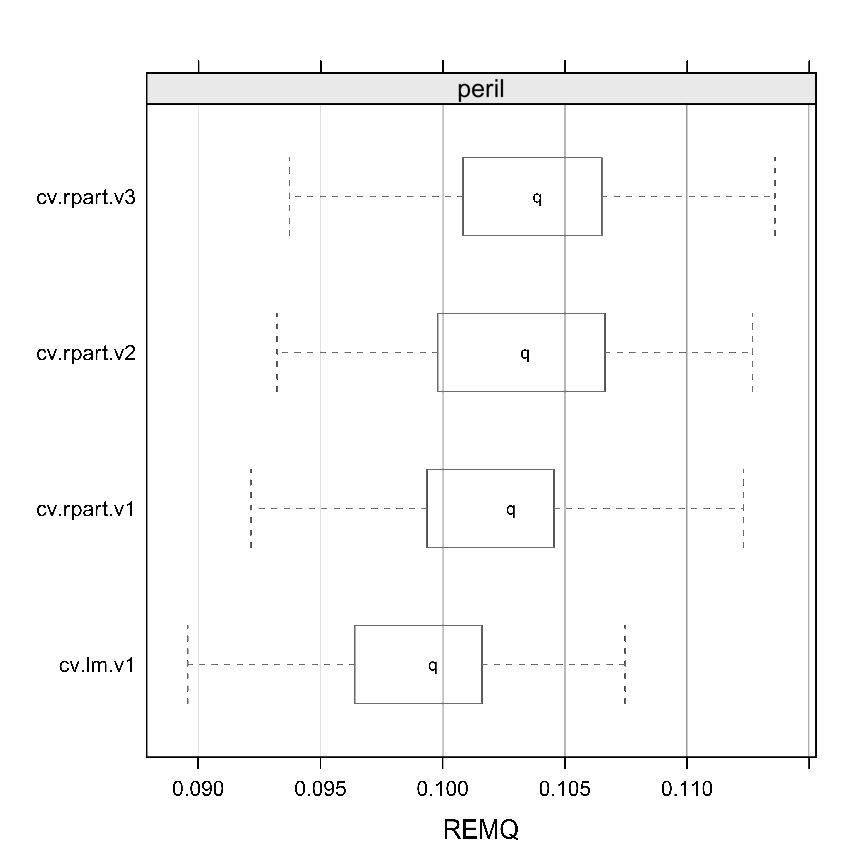
\includegraphics[width=\columnwidth]{image/mrl_ex1.pdf}
  \caption{Boxplots for normalized errors of linear regression models.}
  \label{fig:mlrm_result}
\end{figure}

In Figure \ref{fig:mlrm_result}, normalized RMSE's boxplots after predictions for $RTM_3$, $RTM_2$, $RTM_1$ and MLRM are presented. The minor RMSE is obtained in MLRM, this regression model also has minor standard deviation. From those information, we can affirm MLRM is a more efficient and precise model and will be introduced in the experiment as baseline method.
%Na Figura \ref{fig:mlrm_result}, os \textit{boxplots} da REMQ normalizado após as previsões para MRLM, $MRA_1$, $MRA_2$ e $MRA_3$ são apresentados. O menor REMQ é obtido para o MRLM, esse modelo de regressão também tem menor desvio padrão. A partir dessa informação, pode-se afirmar que o MRLM é um modelo eficiente e preciso e é definido como modelo de linha de base.

\section{Monte Carlo Simulation and PERT Analysis}

%O segundo experimento é analisar o desempenho das técnicas convencionais utilizadas na academia e na indústria, inclusive determinadas como boas práticas pelo PMBOK \cite{PMBOK2008}. Como explicado anteriormente, essas abordagens foram configuradas para obterem o melhor desempenho possível.
The second experiment is to analyze the performance of conventional techniques used in academia and industry, including best practices as determined by PMBOK \cite{PMBOK2008}. As explained earlier, these approaches have been configured to obtain the best possible performance.

%A Tabela \ref{tab:arte_descriptive} mostra a estatística descritiva do REMQ normalizado para ambos os algoritmos. Os valores de média, desvio padrão, mínimo e máximo, calculados para Simulação de Monte Carlo e para a Análise PERT, mostram que a Análise PERT apresenta valores bem inferiores de média, mínimo e máximo. No entanto, o desvio padrão da Simulação de Monte Carlo é menor, provando ser um método mais preciso.
Table \ref{tab:arte_descriptive} shows the descriptive statistics for normalized RMSE for both algorithms. The mean value, standard deviation, minimum and maximum, calculated for Monte Carlo Simulation and PERT Analysis, presents that the PERT Analysis has lower mean, minimum and maximum values. However, MCS has lower standard deviation, proving to be more precise between than.

\begin{table}[h]
\caption{Descriptive statistics for normalized errors of state of art models.}\label{tab:arte_descriptive} \centering
\begin{tabular}{|c|c|c|}
  \hline
   & MCS & PERT \\
  \hline
  Average & 0.12640 & \textbf{0.07466}   \\
  \hline
  Std. Deviation & \textbf{0.01250} & 0.01438   \\
  \hline
  Minimum & 0.10410 & \textbf{0.04788}   \\
  \hline
  Maximum & 0.14950 & \textbf{0.09122}   \\
  \hline
\end{tabular}
\end{table}

\begin{figure}[h]
  \vspace{-0.2cm}
  \centering
  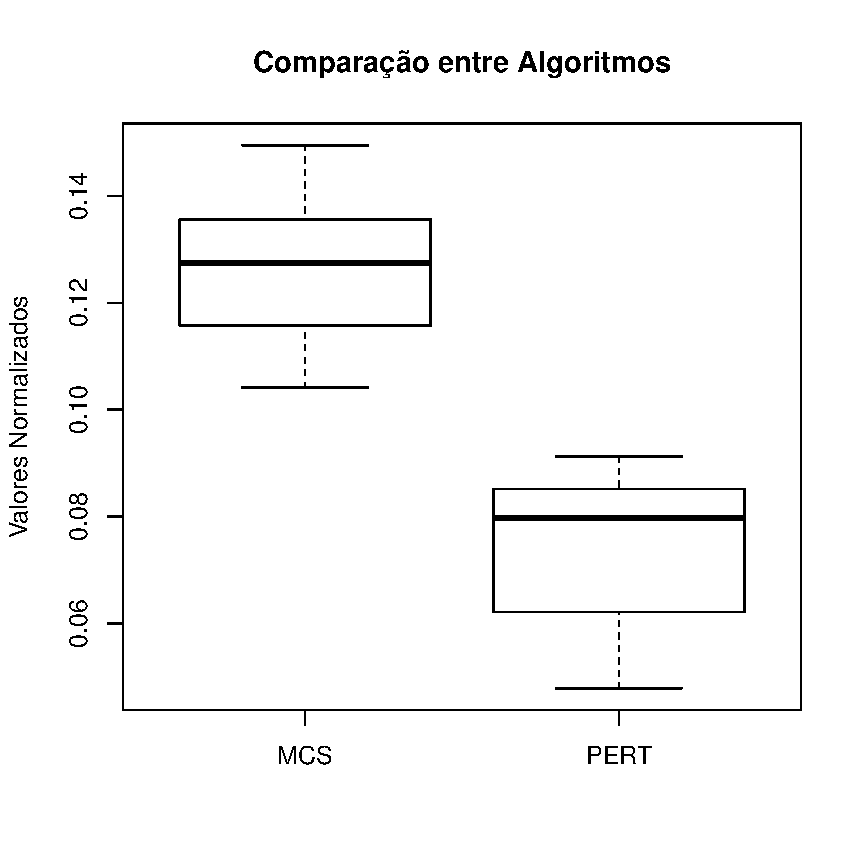
\includegraphics[trim = 1mm 12mm 1mm 1mm,clip,width=0.7\columnwidth]{image/arte_ex2.pdf}
  \caption{Boxplots for normalized errors of linear regression models.}
  \label{fig:arte_result}
\end{figure}

%Na Figura \ref{fig:arte_result}, os \textit{boxplots} da REMQ normalizado após as previsões para SMC e PERT são apresentados. A partir dessa informação, pode-se afirmar que a Análise PERT é um modelo de estado da arte mais eficiente e ligeiramente preciso, nessa comparação.
In Figure \ref{fig:arte_result}, the boxplots of normalized RMSE after forecasts for MCS and PERT are presented. From this information, it can be stated that PERT Analysis is a more efficient state of art and slightly more precise, in this comparison.

%A Análise PERT mostrou ser uma abordagem bastante interessante quando há poucas informações de riscos nas lições aprendidas no gerenciamento de projetos anteriores, como uma base de dados de registro de riscos. Uma análise detalhada utilizando uma base de dados revela que essa técnica apresenta resultados aceitáveis pelos gerentes de projetos.
PERT analysis proved to be a very interesting approach when is little risk information in learned lessons of previous projects, such as a risk register database. A detailed analysis using a database reveals that this technique has acceptable results to project managers.

\section{MultiLayer Perceptron and variations}

%Nesse experimento, algumas MLPs foram avaliadas. A principal diferença entre elas é a regra de aprendizagem. Os algoritmos: \textit{Backpropagation}, Levenberg-Marquardt, Broyden-Fletcher-Goldfarb-Shanno \textit{Backpropagation}, Gradiente Conjugado Escalonado, \textit{Resilient-propagation}, \textit{Resilient-propagation}, \textit{One-step Secant backpropagation} e Quasi-Newton foram alguns dos selecionados.
In this experiment, some MLPs were assessed. The main difference between than is the learning rule; Backpropagation, Levenberg-Marquardt, Broyden-Fletcher-Goldfarb-Shanno Backpropagation, Scaled Conjugate Gradient, Resilient-propagation, One-step Secant backpropagation and Quasi-Newton algorithms sre some of them selected.

%Na Tabela \ref{tab:mlps_descriptive}, é exibida a estatística descritiva do REMQ normalizado para as abordagens desenvolvidas para esse experimento. Os valores de média, desvio padrão, mínimo e máximo são calculados para cada uma das MLPs. "BP" apresenta os resultados para uma MLP com algoritmo de aprendizagem \textit{Backpropagation}; "LM" para uma MLP com o algoritmo Levenberg-Marquardt; "BFGS" para uma MLP com o algoritmo Broyden-Fletcher-Goldfarb-Shanno \textit{Backpropagation}; "SCG" para uma MLP com o algoritmo Gradiente Conjugado Escalonado; "RP" para uma MLP com o algoritmo \textit{Resilient-propagation}; "RPCG" para uma MLP com o algoritmo \textit{Resilient-propagation} combinado com o Gradiente Conjugado; "OSS" para uma MLP com o algoritmo \textit{One-step Secant backpropagation}; por fim, "Reg" para uma MLP chamada "MLPRegressor" com o algoritmo BFGS Quasi-Newton. Conforme os valores médio, mínimo e máximo, observa-se que a alternativa "Reg" é mais eficiente, mesmo tendo o maior desvio padrão segundo esse experimento.
Table \ref{tab:mlps_descriptive} shows off descriptive statistics of normalized RMSE to approaches developed for this experiment. The mean, standard deviation, minimum and maximum values are calculated for each of the MLPs. "BP" shows results for a MLP with backpropagation learning algorithm; "LM" for an MLP with Levenberg-Marquardt algorithm; "BFGS" for an MLP with Broyden-Fletcher-Goldfarb-Shanno Backpropagation algorithm; "SCG" for an MLP with Scaled Conjugate Gradient algorithm; "RP" for an MLP with Resilient-propagation algorithm; "RPCG" for an MLP with Resilient-propagation combined with Conjugate Gradient algorithm; "OSS" for an MLP with One-step Secant backpropagation algorithm. Finally, "Reg" for an MLP called "MLPRegressor" with the BFGS Quasi-Newton algorithm. According to average, minimum and maximum values, it is observed that "Reg" is a more efficient alternative, even with the largest standard deviation second this experiment.

\begin{table}[h]
\caption{Descriptive statistics for normalized errors of MLPs models.}\label{tab:mlps_descriptive} \centering
\begin{tabular}{|c|c|c|c|c|c|c|c|c|}
  \hline
   & BP & LM & BFGS & SCG & RP & RPCG & OSS & Reg \\
  \hline
  Avg & 0.1000 & 0.0986 & 0.0980 & 0.0982 & 0.0979 & 0.0981 & 0.0995 & \textbf{0.0516}   \\
  \hline
  StD & 0.0015 & 0.0018 & \textbf{0.0011} & 0.0018 & 0.0015 & 0.0021 & 0.0031 & 0.0042   \\
  \hline
  Min & 0.0973 & 0.0952 & 0.0945 & 0.0951 & 0.0946 & 0.0950 & 0.0943 & \textbf{0.0427}   \\
  \hline
  Max & 0.1041 & 0.1035 & 0.1004 & 0.1037 & 0.1019 & 0.1041 & 0.1065 & \textbf{0.0603}   \\
  \hline
\end{tabular}
\end{table}

\begin{figure}[h]
  \vspace{-0.2cm}
  \centering
  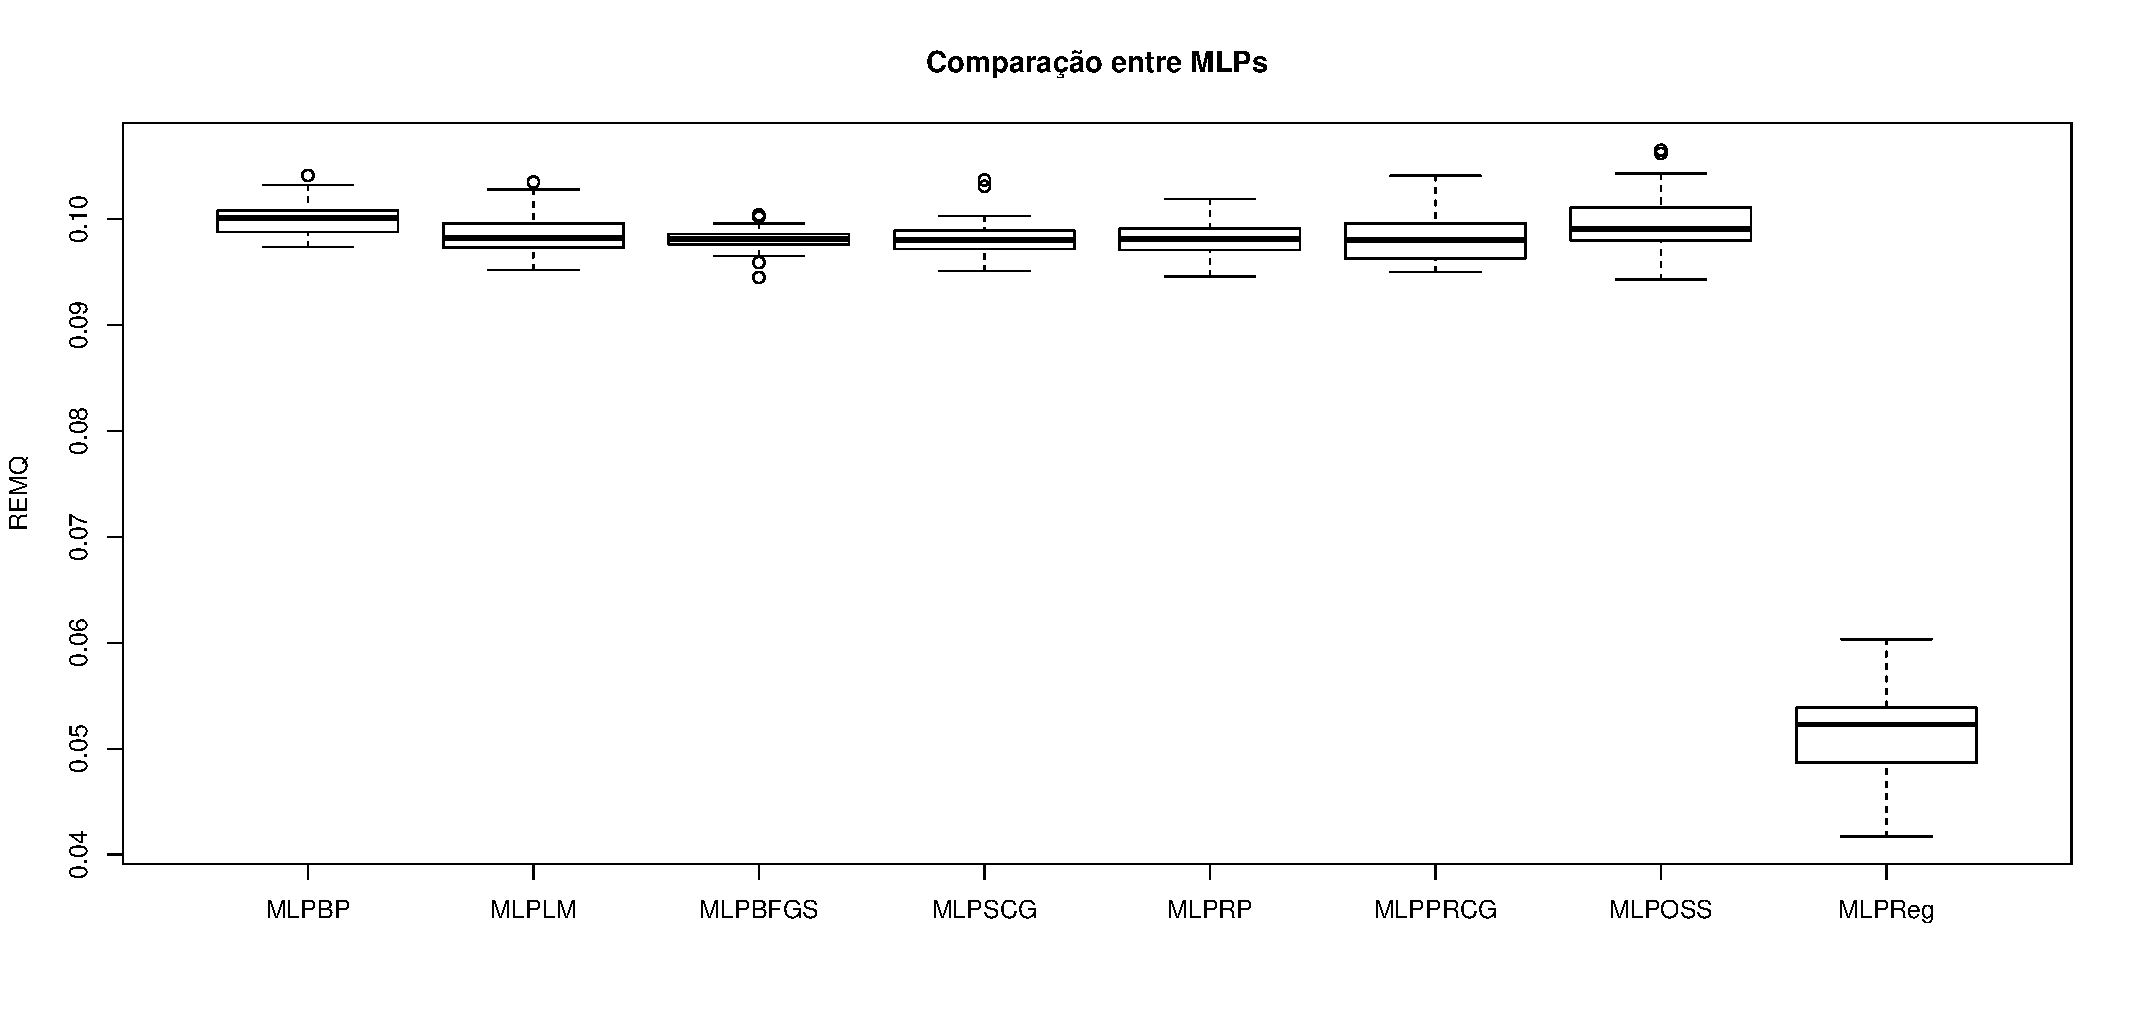
\includegraphics[trim = 1mm 10mm 1mm 1mm,clip,width=\columnwidth]{image/mlps_ex3.pdf}
  \caption{Boxplots for normalized errors of multiple linear perceptron networks.}
  \label{fig:mlps_result}
\end{figure}

%Na Figura \ref{fig:mlps_result}, os \textit{boxplots} da REMQ normalizado após as previsões para as oito MLPs são apresentados. A partir dessas informações, pode-se afirmar que a MLP chamada "MLPRegressor" é uma rede neural mais eficiente porém aidna imprecisa, de acordo com o experimento.
In Figure \ref{fig:mlps_result}, boxplots of normalized RMSE after forecasts for the eight MLPs are presented. From this information, it can be stated that a MLP called "MLPRegressor" is a more efficient but still imprecise artificial neural network, according to experiment.

\section{MLP, SVM, RBF and ANFIS}

%Após avaliar uma rede neural eficiente no experimento anterior, o quarto experimento tem o objetivo de eleger qual a melhor técnica baseada em Redes Neurais Artificiais, dentre as implementadas, para a previsão do impacto de riscos a partir da base de dados PERIL.
After evaluating an efficient neural network in the previous experiment, the fourth experiment aims to elect the best technique based on Artificial Neural Networks, among implemented for predicting risk impact from PERIL database.

%A Tabela \ref{tab:anns_descriptive} mostra a estatística descritiva do REMQ normalizado para as RNAs estudadas. Os valores de média, desvio padrão, mínimo e máximo, calculados para um modelo Neuro-Fuzzy ANFIS, uma SVM (chamada SMORegressor), uma rede RBF (chamada RBFRegressor) e para uma "MLPRegressor" mostram que o último algoritmo apresenta valores bem inferiores de média, mínimo e máximo. No entanto, o desvio padrão do ANFIS é menor. Portanto, "MLPRegressor" prova ser um método mais eficiente e relativamente preciso, em comparação com as outras técnicas, para a estimativa do impacto de risco baseada na PERIL.
Table \ref{tab:anns_descriptive} shows the descriptive statistics for the normalized RMSE to studied ANNs. The mean, standard deviation, minimum and maximum value calculated for a Neuro-Fuzzy model ANFIS, an SVM (called SMORegressor), an RBF network (called RBFRegressor) and for a "MLPRegressor" show that the latter algorithm has much lower average, minimum and maximum values. However, the standard deviation of ANFIS is lower. Therefore, "MLPRegressor" proves to be a relatively efficient and accurate method compared with other techniques to risk impact estimation based on PERIL.

\begin{table}[h]
\caption{Descriptive statistics for normalized errors of ANNs models.}\label{tab:anns_descriptive} \centering
\begin{tabular}{|c|c|c|c|c|}
  \hline
   & ANFIS & SMOReg & RBFReg & MLPReg  \\
  \hline
  Avg & 0.1079 & 0.09430 & 0.09004 & \textbf{0.0516}   \\
  \hline
  StD & \textbf{0.00003} & 0.00488 & 0.00432 & 0.0042   \\
  \hline
  Min & 0.1078 & 0.08347 & 0.08024	 & \textbf{0.0427}   \\
  \hline
  Max & 0.1080 & 0.10284 & 0.09790 & \textbf{0.0603}   \\
  \hline
\end{tabular}
\end{table}

\begin{figure}[!h]
  \vspace{-0.2cm}
  \centering
  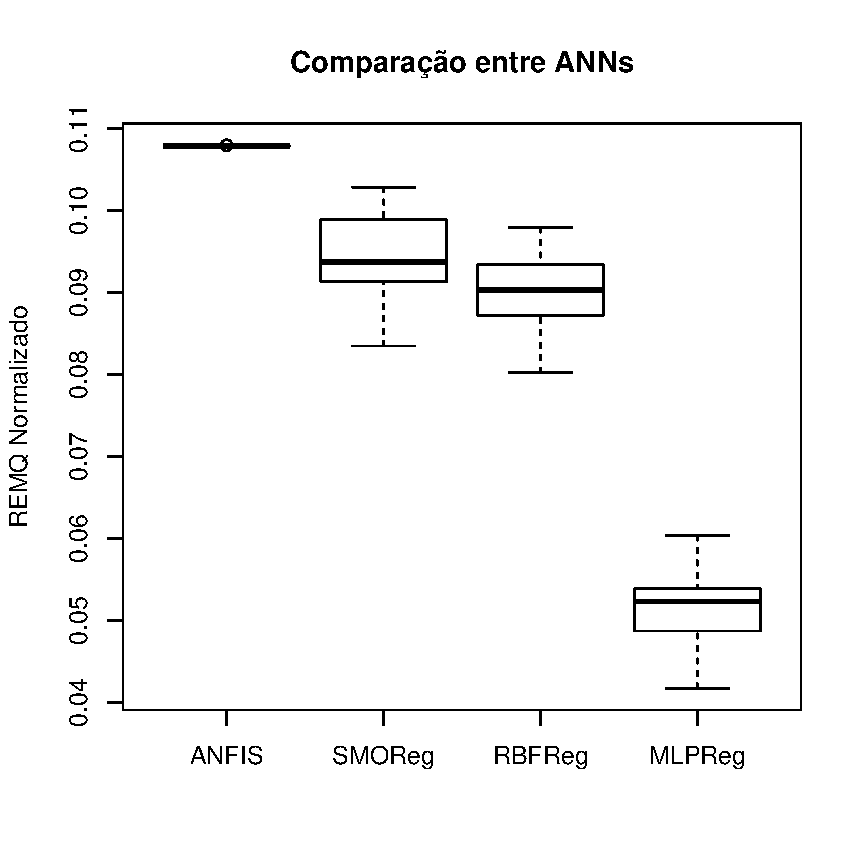
\includegraphics[trim = 1mm 12mm 1mm 1mm,clip,width=0.7\columnwidth]{image/anns_ex4.pdf}
  \caption{Boxplots for normalized errors of ANNs.}
  \label{fig:anns_result}
\end{figure}

%Na Figura \ref{fig:anns_result}, os \textit{boxplots} da REMQ normalizado após as estimativas de impacto das RNAs são apresentados. A partir dessas informações, pode-se afirmar que o "MLPRegressor" é uma Rede Neural Artificial mais eficiente e ligeiramente precisa, de acordo com essa comparação.
In Figure \ref{fig:anns_result}, boxplots of normalized RMSE after impact prediction of RNAs are shown. From this information, it can be stated that the "MLPRegressor" is a more efficient Artificial Neural Network and slightly accurate, according to this comparison.

\begin{figure}[!h]
  \centering
  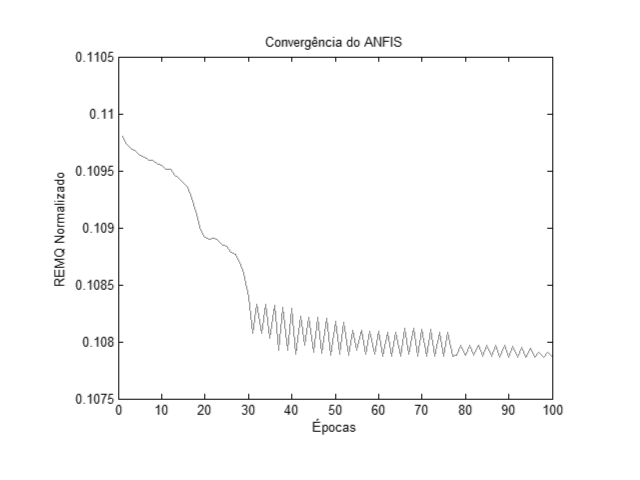
\includegraphics[trim = 1mm 12mm 1mm 8mm,clip,width=\columnwidth]{image/epocas.png}
  \caption{Convergence of ANFIS.}
  \label{fig:anns_result_2}
\end{figure}

%Na Figura \ref{fig:anns_result_2}, é apresentada a convergência do ANFIS, em termos da REMQ normalizado, para cada época durante o treinamento até ser interrompido, de acordo com a validação cruzada. Observa-se que o algoritmo encontra um mínimo local e permanece preso até o treinamento ser interrompido. Logo, conclui-se que o ANFIS apresenta algumas limitações de convergência para essa base de dados.
In Figure \ref{fig:anns_result_2}, the convergence of ANFIS is presented in terms of normalized resched for each season during training to be stopped, according to cross-validation. It is observed that the algorithm finds a local minimum and remains stuck until stopping the training. Therefore, it is concluded that the ANFIS has some limitations on convergence for this database.

\begin{figure}[!h]
  \vspace{-0.2cm}
  \centering
  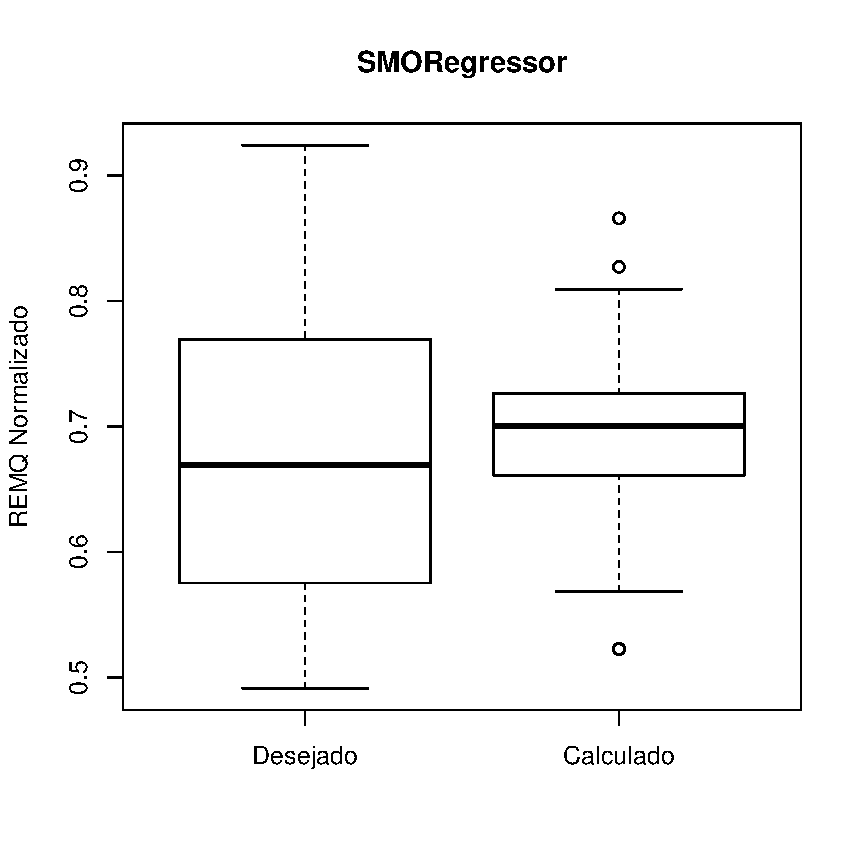
\includegraphics[trim = 1mm 12mm 1mm 1mm,clip,width=0.7\columnwidth]{image/smoreg_ex4.pdf}
  \caption{Boxplots for normalized errors of SVM.}
  \label{fig:anns_result_5}
\end{figure}

%Na Figura \ref{fig:anns_result_5}, os \textit{boxplots} dos impactos esperados e calculados pelo algoritmo "SMORegressor" de cinqunta amostras são apresentados. O resultado ideal é que os \textit{boxplots} das duas amostras sejam o mais semelhantes possível, respeitando a mediana, o intervalo inter-quartil e os valores de mínimo e máximo. A partir da informação apresentada, pode-se concluir que o \textit{boxplot} oriundo dos impactos calculados tenta representar mas distorce em todas as medidas os impactos esperados.
In Figure \ref{fig:anns_result_5}, boxplots of expected and calculated impacts of fifth samples by "SMORegressor" algorithm are presented. The ideal result is boxplots of both samples being as similar as possible, respecting median, interquartile range, minimum and maximum values. From the information presented, it can be concluded that boxplot coming from calculated impacts attempts to represent but distorts in all measures the expected impacts.

\begin{figure}[!h]
  \vspace{-0.2cm}
  \centering
  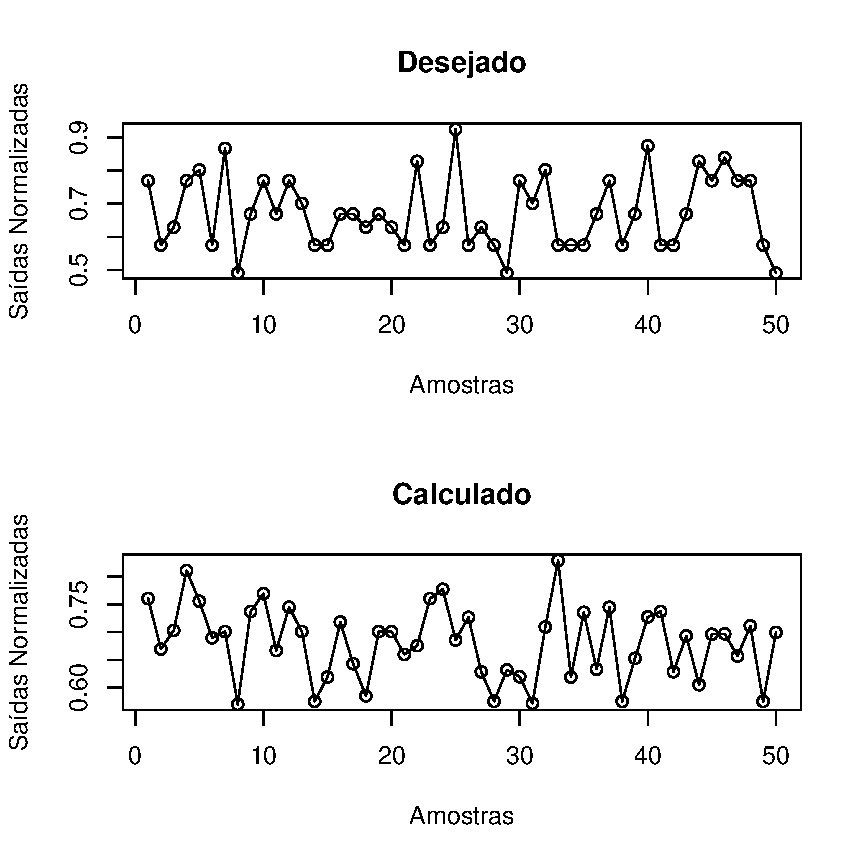
\includegraphics[width=0.7\columnwidth]{image/smoreg_ex4_2.pdf}
  \caption{Normalized errors of expected and calculated impacts.}
  \label{fig:anns_result_6}
\end{figure}

%Na Figura \ref{fig:anns_result_6}, as cinquenta primeiras amostras do subconjunto de testes e da saídas calculadas são apresentadas, graficamente. A partir desses gráficos, pode-se observar que o algoritmo "SMORegressor" tem dificuldade em estimar os resultados esperados, quase não apresentando relação com eles.
In Figure \ref{fig:anns_result_6}, the first fifty samples of expected and calculated outputs are presented graphically. From these graphs, it can be observed that the "SMORegressor" algorithm has difficulty in estimating the expected results, showing almost no relationship with the last ones.

\begin{figure}[!h]
  \vspace{-0.2cm}
  \centering
  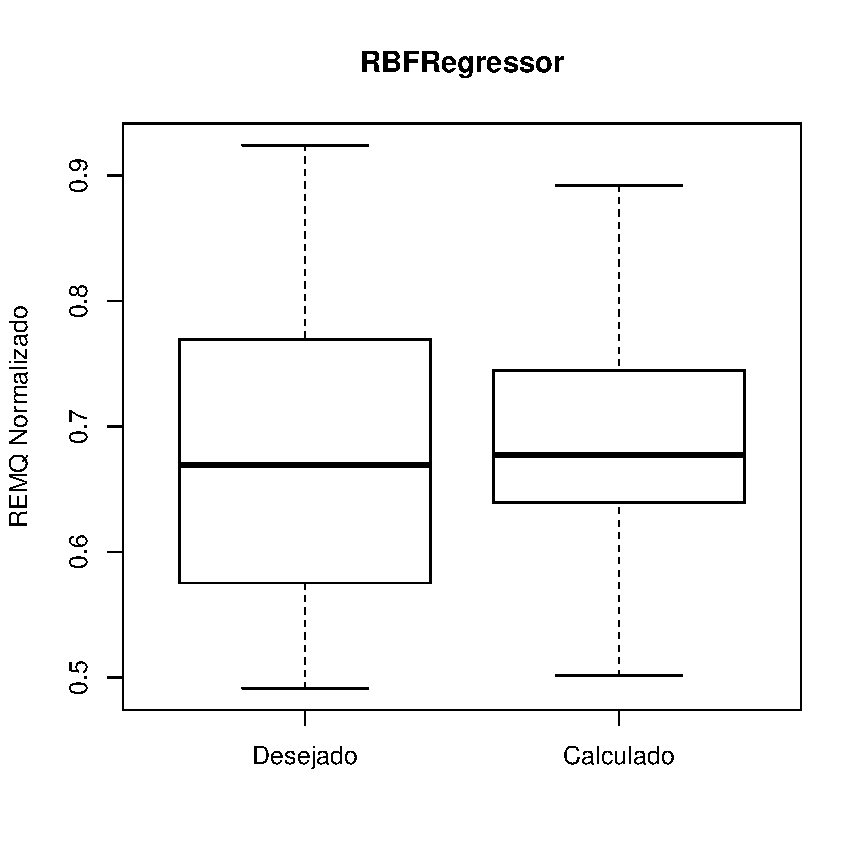
\includegraphics[trim = 1mm 12mm 1mm 1mm,clip,width=0.7\columnwidth]{image/rbfreg_ex4.pdf}
  \caption{Boxplots for normalized errors of RBF networks.}
  \label{fig:anns_result_3}
\end{figure}

%Na Figura \ref{fig:anns_result_3}, os \textit{boxplots} dos impactos esperados e calculados pelo algoritmo "RBFRegressor" de cinquenta amostras são apresentados. O resultado ideal é que os \textit{boxplots} das duas amostras sejam o mais semelhantes possível, respeitando a mediana, o intervalo inter-quartil e os valores de mínimo e máximo. A partir da informação apresentada, pode-se concluir que o \textit{boxplot} oriundo dos impactos calculados tenta representar mas distorce no quartil inferior e nos valores máximos os impactos esperados.
In Figure \ref{fig:anns_result_3}, the boxplots of expected and calculated impacts by "RBFRegressor" of fifth samples are presented. The ideal result is that boxplots of both samples are as similar as possible, respecting the median, interquartile range, minimum and maximum values. From the information presented, it can be concluded that boxplots coming from the calculated impacts attempts but distorts to represent the lower quartile and maximum values of expected impacts. 

\begin{figure}[!h]
  \vspace{-0.2cm}
  \centering
  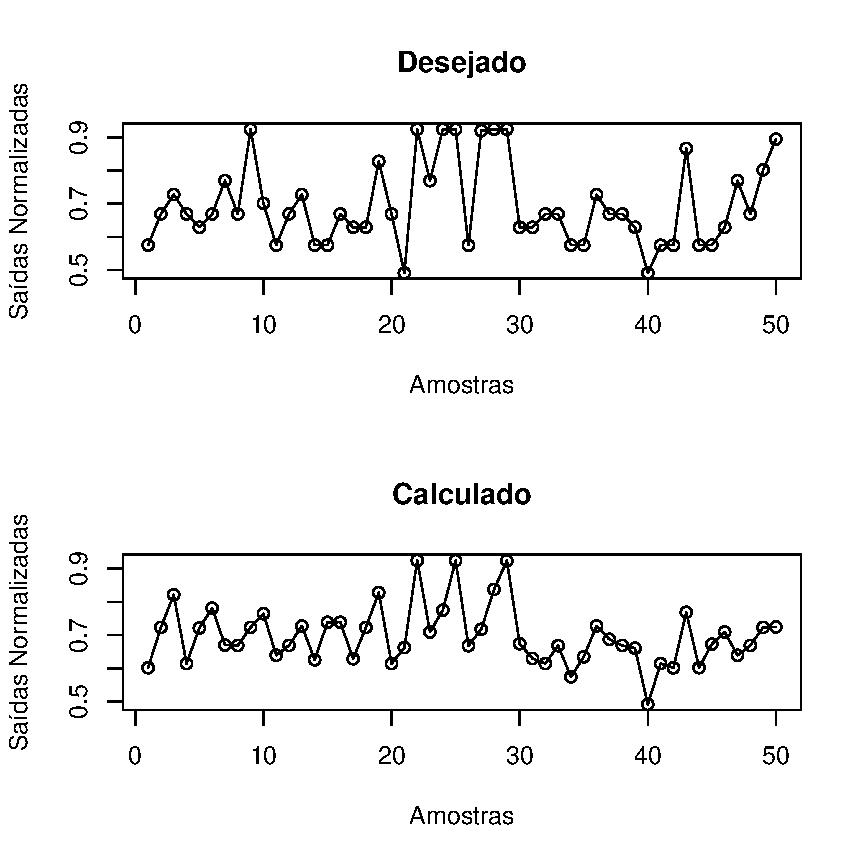
\includegraphics[width=0.7\columnwidth]{image/rbfreg_ex4_2.pdf}
  \caption{Normalized errors of expected and calculated impacts.}
  \label{fig:anns_result_4}
\end{figure}

%Na Figura \ref{fig:anns_result_4}, as cinquenta primeiras amostras do subconjunto de testes e da saídas calculadas são apresentadas, graficamente. A partir desses gráficos, pode-se observar que o algoritmo "RBGRegressor" tem dificuldade em estimar os resultados esperados, principalmente os valores máximos e mínimos.
In Figure \ref{fig:anns_result_4}, the first fifty samples of test subset and calculated outputs are presented graphically. From these graphs, it can be observed that the "RBFRegressor" algorithm has difficulty in estimating the expected outcomes, mainly the maximum and minimum values.

\begin{figure}[!h]
  \vspace{-0.2cm}
  \centering
  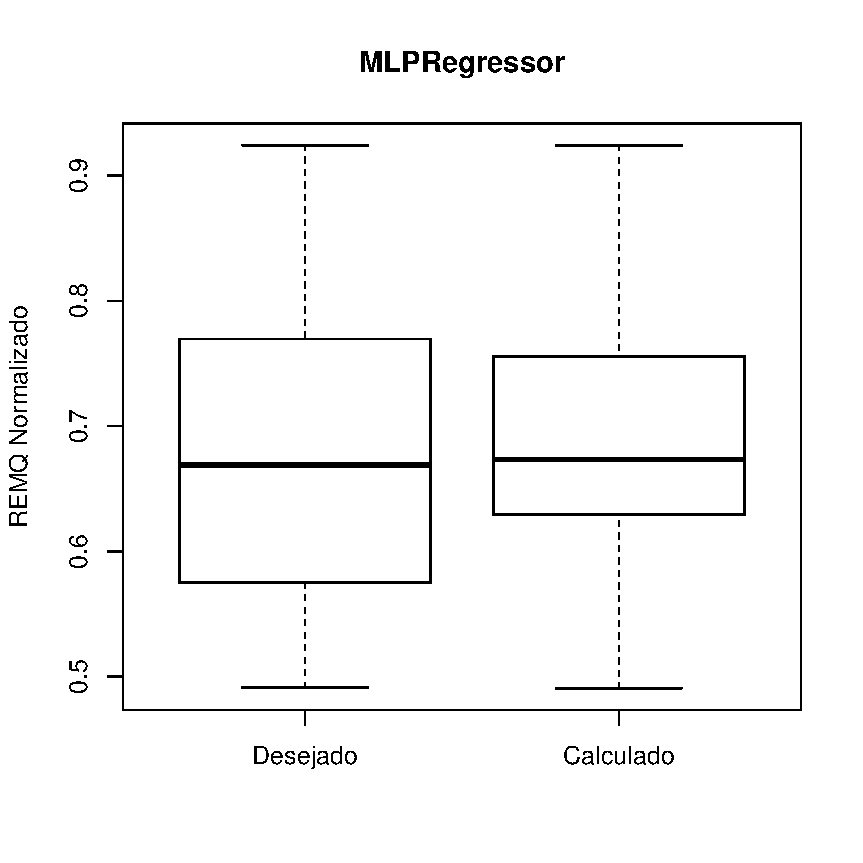
\includegraphics[trim = 1mm 12mm 1mm 1mm,clip,width=0.7\columnwidth]{image/mlpreg_ex4.pdf}
  \caption{Boxplots for normalized errors of expected and calculated outcomes for MLPRegressor.}
  \label{fig:anns_result_7}
\end{figure}

%Na Figura \ref{fig:anns_result_7}, os \textit{boxplots} dos impactos esperados e calculados pelo algoritmo "MLPRegressor" de cinquenta amostras são apresentados. O resultado ideal é que os \textit{boxplots} das duas amostras sejam o mais semelhantes possível, respeitando a mediana, o intervalo inter-quartil e os valores de mínimo e máximo. A partir da informação apresentada, pode-se concluir que o \textit{boxplot} oriundo dos impactos calculados representa, porém com distorções principalmente no quartil inferior, os impactos esperados.
In Figure \ref{fig:anns_result_7}, boxplots of expected impacts and calculated of fifty samples through "MLPRegressor" algorithm are presented. The ideal result is that boxplots of the both samples to be as similar as possible, respecting the median, interquartile range, minimum and maximum values. From the information presented, it can be concluded that boxplot coming from the calculated impacts, but with distortions mainly in the lower quartile represents the expected impacts.

\begin{figure}[!h]
  \vspace{-0.2cm}
  \centering
  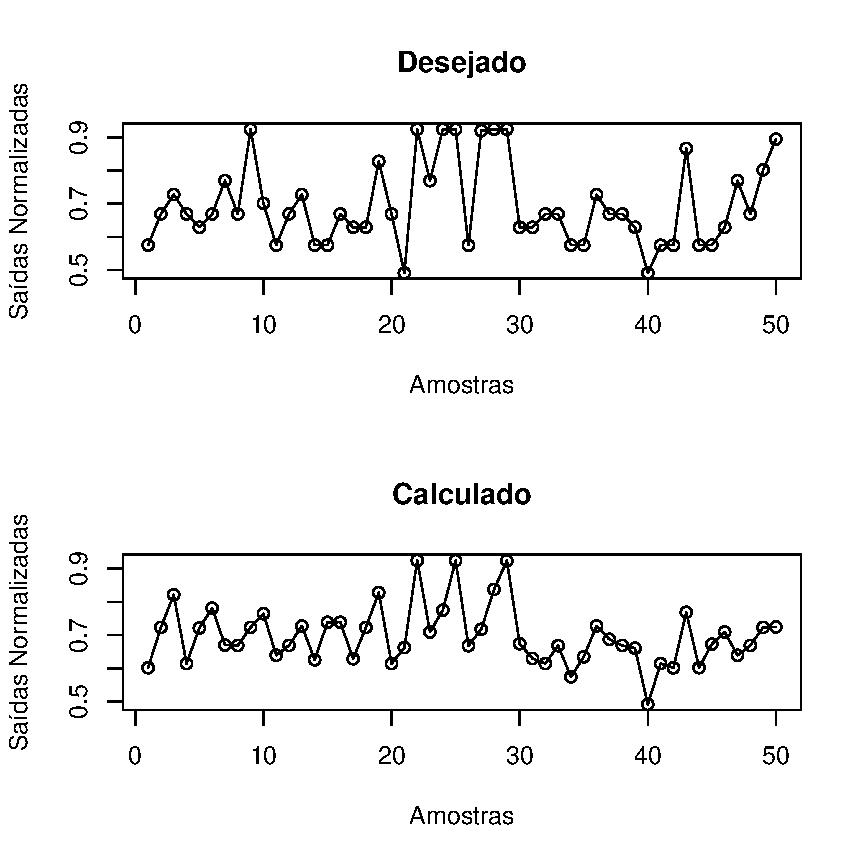
\includegraphics[width=0.7\columnwidth]{image/mlpreg_ex4_2.pdf}
  \caption{Normalized errors of expected and calculated impacts.}
  \label{fig:anns_result_8}
\end{figure}

%Na Figura \ref{fig:anns_result_8}, as cinquenta primeiras amostras do subconjunto de testes e da saídas calculadas são apresentadas, graficamente. A partir desses gráficos, pode-se observar que o algoritmo "MLPRegressor" tem dificuldade em estimar os resultados esperados, porém tende a acompanhar os resultados.
In Figure \ref{fig:anns_result_8}, the first fifty samples of tests subsets and from calculated outputs are presented graphically. From these graphs, it can be observed that "MLPRegressor" algorithm has difficulty in estimating the expected results, but has approximate tendency.

\section{Better Model Validation}

A Tabela \ref{tab:validacao_descriptive} mostra a estatística descritiva do REMQ normalizado para as RNAs estudadas. Os valores de média, desvio padrão, mínimo e máximo, calculados para um MRLM, uma Simulação de Monte Carlo(SMC), uma Análise PERT(PERT) e para uma MLP "MLPRegressor"(MLPReg) mostram que o último algoritmo apresenta valores inferiores de média, desvio padrão, mínimo e máximo. Portanto, "MLPRegressor" prova ser um método mais eficiente e relativamente preciso, em comparação com as outras técnicas, para a estimativa do impacto de risco baseada na PERIL.
%Table \ref{tab:validacao_descriptive} shows descriptive statistics for the normalized RMSE for studied ANNs. Mean, standard deviation, minimum and maximum values calculated for a MLRM, a Monte Carlo Simulation (MCS), a PERT analysis (PERT) and a MLP "MLPRegressor" (MLPReg) show that the latter algorithm has lower mean, standard deviation, minimum and maximum values. Therefore, "MLPRegressor" proves to be a relatively efficient and accurate method compared with other techniques to estimate risk impact based on PERIL.

\begin{table}[h]
\caption{Descriptive statistics for normalized errors of ANNs models.}\label{tab:validacao_descriptive} \centering
\begin{tabular}{|c|c|c|c|c|}
  \hline
   & MLR & MCS & PERT & MLPReg  \\
  \hline
  Avg & 0.09912 & 0.12640 & 0.07466 & \textbf{0.05168}   \\
  \hline
  StD & 0.00794 & 0.01250 & 0.01438 & \textbf{0.00427}   \\
  \hline
  Min & 0.08956 & 0.10410 & 0.04788	 & \textbf{0.04172}   \\
  \hline
  Max & 0.10746 & 0.14950 & 0.09122 & \textbf{0.06035}   \\
  \hline
\end{tabular}
\end{table}

\begin{figure}[!h]
  \vspace{-0.2cm}
  \centering
  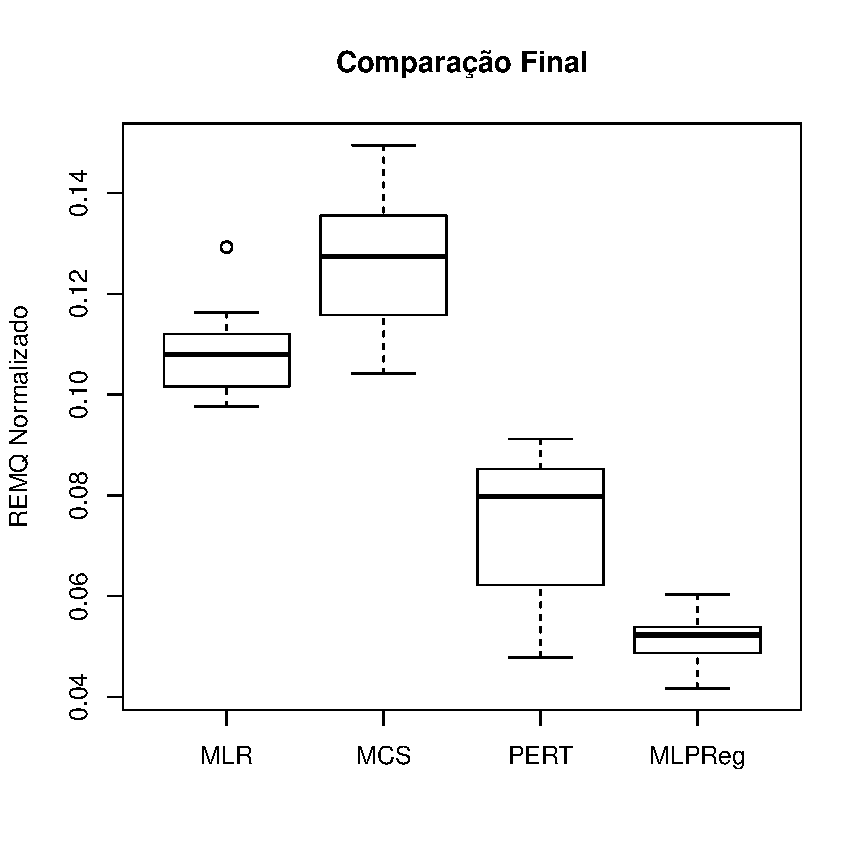
\includegraphics[trim = 1mm 12mm 1mm 1mm,clip,width=0.7\columnwidth]{image/validacao_ex5.pdf}
  \caption{Boxplots for normalized errors of models in validation step.}
  \label{fig:validacao_result}
\end{figure}

%Na Figura \ref{fig:validacao_result}, os \textit{boxplots} da REMQ normalizado após as estimativas de impacto das RNAs são apresentados. A Simulação Monte Carlo(SMC) é imediatamente descartada da análise por apresentar erros maiores que o Modelo de Regressão Linear Múltipla (MLR); a Análise PERT (PERT) apresenta-se como uma abordagem simples e rápida para a estimativa do impacto de riscos, porém como é uma técnica estatística está sujeita a algumas situações que geram maiores erros na estimativa; já, o MLPRegressor (MLPReg) apresenta os menor valores de média, desvio padrão, mínimo e máximo de erro. A partir dessas informações, pode-se afirmar que o "MLPRegressor" é uma Rede Neural Artificial mais eficiente e precisa, comparada com o desempenho das outras RNAs.
In Figure \ref{fig:validacao_result}, boxplots of normalized RMSE after the estimated impact of RNAs are shown. Monte Carlo Simulation (MCS) is immediately discarded from the analysis because it shows higher errors than Multiple Linear Regression Model (MLRM); PERT analysis (PERT) is presented as a simple and fast approach to estimate the risk impact, but as it is a statistical technique is subject to some situations that generate larger errors in the estimation; now, MLPRegressor (MLPReg) presents the lower mean, standard deviation, minimum and maximum error values. From this information, it can be stated that the "MLPRegressor" is an Artificial Neural Network more efficient and accurate compared with the performance of other ANNs and state of art models.

%A Tabela \ref{tab:anns_descriptive} apresenta os resultados dos Testes de Wilcoxon não-pareados para as RNAs estudadas. O símbolo $\Delta$ significa que a técnica à esquerda apresenta melhores resultados que a acima; diferentemente, o símbolo $\nabla$ siginifica que a técnica acima apresenta melhores resultados que à esquerda. Após analisar a tabela, podemos afirmar que a "MLPRegressor" é melhor que a Análise PERT que, por sua vez, é melhor que o Modelo de Regressão Linear Múltipla.
Table \ref{tab: anns_descriptive} presents the results of non-paired Wilcoxon Tests for analyzed ANNs. The symbol $\Delta$ means that the technique on the left shows better results than the above; otherwise, the symbol $\nabla$ simply means that the above technique presents better results than in the left. After analyzing the table, we can see that the "MLPRegressor" is better than the PERT Analysis that, in turn, is better than the Multiple Linear Regression Model.

%Teste de Hipótese
\begin{table}[h]
\caption{Hypothesis Tests for analyzed ANNs.}\label{tab:teste_hipotese} \centering
\begin{tabular}{|c|c|c|c|c|}
  \hline
   & MLR & MCS & PERT & MLPReg  \\
  \hline
  MLR & - & $\Delta$ & $\nabla$ & $\nabla$   \\
  \hline
  MCS & $\nabla$ & - & $\nabla$ & $\nabla$   \\
  \hline
  PERT & $\Delta$ & $\Delta$ & - & $\nabla$   \\
  \hline
  MLPReg & $\Delta$ & $\Delta$ & $\Delta$ & -   \\
  \hline
\end{tabular}
\end{table}

\section{Impact Estimation and Confidence Interval Definition}

%O último experimento consiste na aplicação prática da metodologia proposta nesse estudo, com base no PERIL. Como alguns passos descritos na metodologia foram seguidos nos experimentos anteriores, resta somente a geração de um intervalo de confiança que é a informação compreendida pelos gerentes de projetos, analistas de projetos e de riscos.
The last experiment consists in the practical used of the methodology proposed in this study, based on PERIL. As some steps described in the methodology were conducted in previous experiments, there remains only the generation of a confidence interval that is information understood by project managers and project and risk analysts.

%A aplicação do intervalo de confiança irá determinar a qualidade dos resultados gerados. A partir dos resultados apresentados pelo modelo, será gerado um intervalo que, para uma determinada previsão, terá 95 \% de chances de conter o valor real. Para isso, será utilizado o método de máxima verossimilhança.
The use of the confidence interval will determine the quality of the results generated. From the results shown by the model, will be generated a range that, for a given provision, will be 95 \% chance of containing the true value. For this, maximum likelihood method will be used.

%O método de máxima verossimilhança considera que existem duas fontes de incertezas para um modelo de previsão. O primeiro, o $\sigma_v$, é a variância do ruído, e o segundo, $\sigma_w$, é a variância da incerteza. O $\sigma_v$ representa a variância dos erros gerados pelo conjunto de validação cruzada na fase de treinamento. Esses valores seguem uma distribuição normal e possuem média zero. Já o $\sigma_w$ é referente à variância de incerteza do modelo e é calculada a partir da utilização do modelo para prever os erros gerados pela própria rede.
The maximum likelihood method considers that there are two sources of uncertainty in a forecast model. The first, $\sigma_v$ is the noise variance, and the second, $\sigma_w$, is the variance of uncertainty. The $\sigma_v$ is the variance of the errors generated by the set of cross-validation in the training phase. Those values follow a normal distribution and average to zero. But, $\sigma_w$ refers to the variance of model uncertainty and is calculated from the use of the model to predict the errors generated by the network itself.

%Assume-se que essas duas fontes de erro são independentes. Então o cálculo da variância total do modelo é dado pela Equação \ref{eq:var_intervalo}.
It is assumed that these two sources of error are independent. Then the calculation of the total variance for the model is given by Equation \ref{eq:var_intervalo}.

\begin{equation}
\label{eq:var_intervalo}
\sigma^{2}_{total} = \sigma^{2}_{v} + \sigma^{2}_{w}
\end{equation}

No processo de validação cruzada do modelo, calcula-se o $\sigma_v$ que é a variância dos erros. Para cada entrada do conjunto calcula-se o erro e ao final do processo a média desses erros e extrai-se sua variância usando a Equação \ref{eq:var_validacao}.
%In cross-validation process of the model, it is calculated the $\sigma_v$ that is the variance of errors. For each input in set the error is calculated, at the end of the process the average of these errors is calculated and its variance is obtained using Equation \ref{eq:var_validacao}.

\begin{equation}
\label{eq:var_validacao}
\sigma_v = \frac{1}{n-1} \sum_{n}^{i=1} (Erro_i - \overline{Erro})^2
\end{equation}

%onde, $n$ é a quantidade de valores; $Erro_i$ é o erro referente à entrada i; $\overline{Erro}$ é a média dos erros.
where, $n$ is the number of values; $Erro_i$ is the error correspondent to input $i$; $\overline{Erro}$ is the error average.

%Para calcular o $\sigma_w$, armazena-se is erros para todas as entrada utilizadas no treinamento da rede, incluindo dados de treinamento e validação cruzada. com esses dados devidamente armazenados e normalizados, cria-se um novo modelo, com novos pesos e novas ligações. Esse modelo terá como objetivo, ou seja, valores desejados, os erros gerados pelo modelo anterior. O $\sigma_w$ será calculado utilizando a mesma fórmula utilizada para o $\sigma_v$. A diferença está na quantidade de dados, pois, para o $\sigma_w$ serão utilizados todos os erros de todos os conjuntos, não só o de validação cruzada.
To calculate $\sigma_w$, errors are stored for all utilized inputs in training, including those in cross-validation subset. Since data are stored and normalized, a new model is obtained with new weights and links. This model will have as desired values the errors generated by the previous model. The $\sigma_w$ will be calculated using the same formula used for the $\sigma_v$. The difference is the amount of data because, $\sigma_w$ uses all errors of all subsets, not only the cross-validation.

%Tendo o $\sigma_v$ e $\sigma_w$ calculados, pode-se calcular o $\sigma_total$. Este será utilizado para calcular o intervalo de confiança a partir da Equação \ref{eq:intervalo_confianca}.
Since $\sigma_v$ and $\sigma_w$ are calculated, one can calculate $\sigma_{total}$. This will be used to calculate the confidence interval from Equation \ref{eq:intervalo_confianca}.

\begin{equation}
\label{eq:intervalo_confianca}
x - t * \sigma_total < x < x + t * \sigma_total
\end{equation}

%onde, $x$ é o valor calculado pela rede e $t$ é o valor extraído da tabela de t de Student para o maior grau de liberdade possível para um intervalo de 95\% de chances de conter o valor real, como exibido na Tabela \ref{tab:lm_descriptive}.
where $x$ is the computed outcome by the network and $t$ is the value extracted from the Student's T table to the largest possible degree of freedom for a period of 95 \% chance of containing the true value, as shown in table \ref{tab:lm_descriptive}.

\begin{table}[h]
\caption{A briefing of Student's T table.}\label{tab:t-student} \centering
\begin{tabular}{|c|c|c|c|c|}
  \hline
  \multicolumn{5}{|c|}{$P(t_n \leq x)$}  \\
  \hline
  \textbf{n} & 0,750 & 0,900 & 0,950 & 0,975  \\
  \hline
  30 & 0,683 & 1,310 & 1,697 & 2,042   \\
  \hline
  40 & 0,681 & 1,303 & 1,684 & 2,021   \\
  \hline
  60 & 0,679 & 1,296 & 1,671 & 2,000   \\
  \hline
  120 & 0,677 & 1,289 & 1,658 & 1,980   \\
  \hline
  $\infty$ & 0,674 & 1,284 & 1,645 & \textbf{1,960}   \\
  \hline
\end{tabular}
\end{table}

\pagebreak

  \chapter{Conclusões e Trabalhos Futuros}\label{cap:conclusion}

Este trabalho investigou o uso de redes neurais artificiais, como algoritmos SVM e MLP, para a estimativa do impacto do risco, através da proposta de uma metodologia para a análise de risco em projetos de \textit{software}, a partir de dados históricos de registros de riscos. 

Os resultados mostraram que as redes neurais artificiais apresentaram resultados promissores, principalmente porque um modelo MLP chamado ``MLPRegressor" obteve os menores erros de previsão. Além disso, alguns resultados apresentaram informações importantes: a SMC apresentou resultados piores comparado com o modelo de linha de base, o MRLM; o modelo ANFIS apresentou resultados piores comparado com a "MLPRegressor", porém é mais preciso 52\% na média comparado com o último modelo; é difícil melhorar ainda mais o desempenho da Análise PERT e da SMC já que todas as medidas foram tomadas para que com as informações disponíveis esses modelos pudessem apresentar os melhores resultados.

Além disso, uma pesquisa rápida realizada com duzentos profissionais (membros da comunidade de prática de gerenciamento de risco do PMI, dos mais diversos campos de aplicação e setores), os quais dez responderam às perguntas feitas, informaram que, no geral, entre 0\% e 5\% é um intervalo de erros ideal de previsão de impacto de risco; 5\% e 10\% é um intervalo aceitável de erro na estimativa e 10\% e 15\% é um intervalo indesejado. Portanto, como o ``MLPRegressor" apresentou alguns valores no primeiro intervalo, REMQ médio de 0.05168 ou 5,168\%, é possível afirmar que esse modelo apresenta resultados satisfatórios.

% Listar os problemas e dificuldades encontradas
Algumas dificuldades foram encontradas nesse estudo, principalmente quanto ao pré-processamento dos dados e a seleção das redes neurais e suas variações para se obter os resultados desejados. Porque não há qualquer trabalho científico utilizando a PERIL para se tomar como base, segundo a revisão bibliográfica feita.

Alguns resultados interessantes foram alcançados porém é preciso melhorar algumas técnicas utilizadas para que os resultados possam ser mais precisos e menores erros de previsão sejam obtidos. Além disso, há uma carga computacional elevada no procedimento de utilização de um algoritmo de otimização para otimizar o desempenho das redes neurais, o que demanda tempo. Como atividades futuras, foram identificadas:
\begin{itemize}
\item Realizar a validação prática dessa metodologia com informações reais para a estimativa e acompanhamento de riscos;
\item Desenvolver uma abordagem eficiente e precisa para quando houver poucas informações sobre os riscos identificados num projeto e nenhum registro de riscos em projetos similares anteriores;
\item Desenvolver uma abordagem inovadora e mais eficiente para a análise qualitativa dos riscos, baseada na classificação da natureza dos riscos;
\item Desenvolver uma técnica para a avaliação de estratégias de mitigação de risco, baseadas no impacto se o risco ocorrer, no esforço para mitigação de risco, nas interações entre os fatores de risco e nos recursos disponíveis para os planos de mitigação;
\item Desenvolver uma metodologia para a avaliação qualitativa, a avaliação quantitativa e planos de contingência de riscos em projetos, do ponto de vista do gerenciamento de portfólio de projetos para o alcance de objetivos estratégicos.
\item Desenvolvimento de um \textit{canvas} para o gerenciamento de riscos em projetos de forma ágil;
\item Implementar outros métodos de validação cruzada.
\end{itemize}

\pagebreak


  \chapter*{Appendix A}


\textbf{Publications:}
\\
\\


\textbf{Title:} A Cooperative Approach using Particle Swarm Optimization with Adaptive Behavior.

\textbf{Authors:} L. N. Vitorino, S. F. Ribeiro and C. J. A. Bastos-Filho.

\textbf{Published in:} 10th Brazilian Congress on Computational Intelligence (CBIC'2011), pages 1-8, 2011.

\textbf{Abstract:}Particle Swarm Optimization (PSO) has been widely used to solve real world optimization problems. Since the original PSO fails to maintain the diversity along the search process, some PSO variations have been proposed to overcome this limitation. The recently introduced Adaptive Particle Swarm Optimization (APSO) presents faster convergence, while maintaining the population diversity, by including into the PSO algorithm the auto-adaptation of the parameters according to the current spatial distribution of the swarm. Besides, there are some PSO variations which incorporate a cooperative behavior, such as the Clan Particle Swarm Optimization (ClanPSO). In this paper, we propose to include the auto-adaptation ability solely in the Clans of the ClanPSO algorithm and compare its performance to previous approaches. We evaluated our proposal in six benchmark functions recently proposed in IEEE Congress on Evolutionary Computation 2010. Our proposal obtained similar or better results in terms of fitness when compared to the original ClanAPSO, but presents a lower computational cost. We obtained better results when compared to other cooperative approaches and the classical PSO approaches.

\

\
\textbf{Title:} A Hybrid Swarm Intelligence Optimizer based on Particles and Artificial Bees for High-Dimensional Search Spaces.

\textbf{Authors:} L. N. Vitorino, S. F. Ribeiro and C. J. A. Bastos-Filho.

\textbf{Published in:} IEEE Congress on Evolutionary Computation 2012 (CEC'2012), 381-386, 2012.

\textbf{Abstract:} Real-world problems can present search spaces with hundreds of dimensions and swarm intelligence algorithms have been developed to solve this type of problems. Particle Swarm Optimization (PSO) presents a fast convergence in continuous problems, but it cannot maintain diversity along the search process. On the other hand, Artificial Bee Colony (ABC) presents the capability to generate diversity when the guide bees are in the exploration mode. We propose in this paper to introduce a mechanism based on the ABC to generate diversity in an adaptive PSO approach and analyze its performance in high dimensional search spaces. The swarm switches its behavior depending on the dispersion of the swarm. We evaluated our proposal in a well known set of 20 benchmark functions recently proposed in 2010
and our proposal achieved better performance than PSO, APSO and ABC in most of the cases.

\

\
\textbf{Title:} A Mechanism based on Artificial Bee Colony to Generate Diversity in Particle Swarm Optimization.

\textbf{Authors:} L. N. Vitorino, S. F. Ribeiro and C. J. A. Bastos-Filho.

\textbf{Published in:} The 3rd International Congress on Swarm Intelligence, 2012.

\textbf{Abstract:} Particle Swarm Optimization (PSO) presents a fast convergence in continuous problems, but it cannot maintain diversity along the entire search process. On the other hand, Artificial Bee Colony (ABC) presents the capability to generate diversity when the guide bees are in the exploration mode. We propose in this paper to introduce a mechanism based on the ABC to generate diversity when the PSO stagnates. The swarm entities switches between two pre-defined behaviors depending on the evolutionary state. We used the Adaptive PSO variation since it presents better adaptation capabilities and it also has a mechanism to evaluate the evolutionary state. We evaluated our proposal for all benchmark functions recently proposed for large scale optimization in CEC2010 and our proposal achieved better performance in most of the cases.


\textbf{Observation:} This paper was selected to Special Issue entitled "Swarm Intelligence for Neural Networks" (Special Issue: SINN 2012) in Neurocomputing (famous SCI-indexed Journal, IF=1.429).
\

\



\pagebreak

% Thesis Chapters [END]

% Bibliography [START]
  \bibliographystyle{alpha}
  \bibliography{ppgec}
% Bibliography [END]
\end{document}
